\chapter{Computing with Register Machines}
\label{Chapter 5}

\dictum[
	Johannes Kepler (letter to Herwart von Hohenburg, 1605)
]{
	My aim is to show that the heavenly machine is not a kind of divine, live being, but a kind of clockwork (and he who believes that a clock has soul attributes the maker’s glory to the work), insofar as nearly all the manifold motions are caused by a most simple and material force, just as all motions of the clock are caused by a single weight.
}


\vspace{2em}


\noindent
\lettrine[findent=1pt]{W}{e began this book} by studying processes and by describing processes in terms of procedures written in Lisp.
To explain the meanings of these procedures, we used a succession of models of evaluation:
the substitution model of \cref{Chapter 1}, the environment model of \cref{Chapter 3}, and the metacircular evaluator of \cref{Chapter 4}.
Our examination of the metacircular evaluator, in particular, dispelled much of the mystery of how Lisp-like languages are interpreted.
But even the metacircular evaluator leaves important questions unanswered, because it fails to elucidate the mechanisms of control in a Lisp system.
For instance, the evaluator does not explain how the evaluation of a subexpression manages to return a value to the expression that uses this value, nor does the evaluator explain how some recursive procedures generate iterative processes (that is, are evaluated using constant space) whereas other recursive procedures generate recursive processes.
These questions remain unanswered because the metacircular evaluator is itself a Lisp program and hence inherits the control structure of the underlying Lisp system.
In order to provide a more complete description of the control structure of the Lisp evaluator, we must work at a more primitive level than Lisp itself.

In this chapter we will describe processes in terms of the step-by-step operation of a traditional computer.
Such a computer, or \newterm{register machine}, sequentially executes \newterm{instructions} that manipulate the contents of a fixed set of storage elements called \newterm{registers}.
A typical register-machine instruction applies a primitive operation to the contents of some registers and assigns the result to another register.
Our descriptions of processes executed by register machines will look very much like “machine-language” programs for traditional computers.
However, instead of focusing on the machine language of any particular computer, we will examine several Lisp procedures and design a specific register machine to execute each procedure.
Thus, we will approach our task from the perspective of a hardware architect rather than that of a machine-language computer programmer.
In designing register machines, we will develop mechanisms for implementing important programming constructs such as recursion.
We will also present a language for describing designs for register machines.
In \cref{Section 5.2} we will implement a Lisp program that uses these descriptions to simulate the machines we design.

Most of the primitive operations of our register machines are very simple.
For example, an operation might add the numbers fetched from two registers, producing a result to be stored into a third register.
Such an operation can be performed by easily described hardware.
In order to deal with list structure, however, we will also use the memory operations \code{car}, \code{cdr}, and \code{cons}, which require an elaborate storage-allocation mechanism.
In \cref{Section 5.3} we study their implementation in terms of more elementary operations.

In \cref{Section 5.4}, after we have accumulated experience formulating simple procedures as register machines, we will design a machine that carries out the algorithm described by the metacircular evaluator of \cref{Section 4.1}.
This will fill in the gap in our understanding of how Scheme expressions are interpreted, by providing an explicit model for the mechanisms of control in the evaluator.
In \cref{Section 5.5} we will study a simple compiler that translates Scheme programs into sequences of instructions that can be executed directly with the registers and operations of the evaluator register machine.

\section{Designing Register Machines}
\label{Section 5.1}

To design a register machine, we must design its \newterm{data paths} (registers and operations) and the \newterm{controller} that sequences these operations.
To illustrate the design of a simple register machine, let us examine Euclid’s Algorithm, which is used to compute the greatest common divisor (\acronym{GCD}) of two integers.
As we saw in \link{Section 1.2.5}, Euclid’s Algorithm can be carried out by an iterative process, as specified by the following procedure:
\begin{scheme}
	(define (gcd a b)
	  (if (= b 0)
	      a
	      (gcd b (remainder a b))))
\end{scheme}

A machine to carry out this algorithm must keep track of two numbers, \( a \) and \( b \), so let us assume that these numbers are stored in two registers with those names.
The basic operations required are testing whether the contents of register \code{b} is zero and computing the remainder of the contents of register \code{a} divided by the contents of register \code{b}.
The remainder operation is a complex process, but assume for the moment that we have a primitive device that computes remainders.
On each cycle of the \acronym{GCD} algorithm, the contents of register \code{a} must be replaced by the contents of register \code{b}, and the contents of \code{b} must be replaced by the remainder of the old contents of \code{a} divided by the old contents of \code{b}.
It would be convenient if these replacements could be done simultaneously, but in our model of register machines we will assume that only one register can be assigned a new value at each step.
To accomplish the replacements, our machine will use a third “temporary” register, which we call \code{t}.
(First the remainder will be placed in \code{t}, then the contents of \code{b} will be placed in \code{a}, and finally the remainder stored in \code{t} will be placed in \code{b}.)

We can illustrate the registers and operations required for this machine by using the data-path diagram shown in \link{Figure 5.1}.
In this diagram, the registers (\code{a}, \code{b}, and \code{t}) are represented by rectangles.
Each way to assign a value to a register is indicated by an arrow with an \code{X} behind the head, pointing from the source of data to the register.
We can think of the \code{X} as a button that, when pushed, allows the value at the source to “flow” into the designated register.
The label next to each button is the name we will use to refer to the button.
The names are arbitrary, and can be chosen to have mnemonic value (for example, \code{a←b} denotes pushing the button that assigns the contents of register \code{b} to register \code{a}).
The source of data for a register can be another register (as in the \code{a←b} assignment), an operation result (as in the \code{t←r} assignment), or a constant (a built-in value that cannot be changed, represented in a data-path diagram by a triangle containing the constant).

\begin{figure}[tb]
	\centering
	\includesvg[width=58mm]{fig/chap5/Fig5.1a.svg}
	\caption{
		Data paths for a \acronym{GCD} machine.
	}
	\label{Figure 5.1}
\end{figure}

An operation that computes a value from constants and the contents of registers is represented in a data-path diagram by a trapezoid containing a name for the operation.
For example, the box marked \code{rem} in \link{Figure 5.1} represents an operation that computes the remainder of the contents of the registers \code{a} and \code{b} to which it is attached.
Arrows (without buttons) point from the input registers and constants to the box, and arrows connect the operation’s output value to registers.
A test is represented by a circle containing a name for the test.
For example, our \acronym{GCD} machine has an operation that tests whether the contents of register \code{b} is zero.
A test also has arrows from its input registers and constants, but it has no output arrows;
its value is used by the controller rather than by the data paths.
Overall, the data-path diagram shows the registers and operations that are required for the machine and how they must be connected.
If we view the arrows as wires and the \code{X} buttons as switches, the data-path diagram is very like the wiring diagram for a machine that could be constructed from electrical components.

\begin{figure}[tb]
	\centering
	\includesvg[width=41mm]{fig/chap5/Fig5.2.svg}
	\caption{
		Controller for a \acronym{GCD} machine.
	}
	\label{Figure 5.2}
\end{figure}

In order for the data paths to actually compute \acronym{GCD}s, the buttons must be pushed in the correct sequence.
We will describe this sequence in terms of a controller diagram, as illustrated in \link{Figure 5.2}.
The elements of the controller diagram indicate how the data-path components should be operated.
The rectangular boxes in the controller diagram identify data-path buttons to be pushed, and the arrows describe the sequencing from one step to the next.
The diamond in the diagram represents a decision.
One of the two sequencing arrows will be followed, depending on the value of the data-path test identified in the diamond.
We can interpret the controller in terms of a physical analogy:
Think of the diagram as a maze in which a marble is rolling.
When the marble rolls into a box, it pushes the data-path button that is named by the box.
When the marble rolls into a decision node (such as the test for \code{b} = 0), it leaves the node on the path determined by the result of the indicated test.
Taken together, the data paths and the controller completely describe a machine for computing \acronym{GCD}s.
We start the controller (the rolling marble) at the place marked \code{start}, after placing numbers in registers \code{a} and \code{b}.
When the controller reaches \code{done}, we will find the value of the \acronym{GCD} in register \code{a}.



\begin{exercise}
	\label{Exercise 5.1}
	Design a register machine to compute factorials using the iterative algorithm specified by the following procedure.
	Draw data-path and controller diagrams for this machine.
	\begin{scheme}
	  (define (factorial n)
	    (define (iter product counter)
	      (if (> counter n)
	          product
	          (iter (* counter product)
	                (+ counter 1))))
	    (iter 1 1))
	\end{scheme}
\end{exercise}



\subsection{A Language for Describing Register Machines}
\label{Section 5.1.1}

Data-path and controller diagrams are adequate for representing simple machines such as \acronym{GCD}, but they are unwieldy for describing large machines such as a Lisp interpreter.
To make it possible to deal with complex machines, we will create a language that presents, in textual form, all the information given by the data-path and controller diagrams.
We will start with a notation that directly mirrors the diagrams.

We define the data paths of a machine by describing the registers and the operations.
To describe a register, we give it a name and specify the buttons that control assignment to it.
We give each of these buttons a name and specify the source of the data that enters the register under the button’s control.
(The source is a register, a constant, or an operation.)
To describe an operation, we give it a name and specify its inputs (registers or constants).

We define the controller of a machine as a sequence of \newterm{instructions} together with \newterm{labels} that identify \newterm{entry points} in the sequence.
An instruction is one of the following:
\begin{itemize}

	\item
		The name of a data-path button to push to assign a value to a register.
		(This corresponds to a box in the controller diagram.)

	\item
		A \code{test} instruction, that performs a specified test.

	\item
		A conditional branch (\code{branch} instruction) to a location indicated by a controller label, based on the result of the previous test.
		(The test and branch together correspond to a diamond in the controller diagram.)
		If the test is false, the controller should continue with the next instruction in the sequence.
		Otherwise, the controller should continue with the instruction after the label.

	\item
		An unconditional branch (\code{goto} instruction) naming a controller label at which to continue execution.

\end{itemize}
The machine starts at the beginning of the controller instruction sequence and stops when execution reaches the end of the sequence.
Except when a branch changes the flow of control, instructions are executed in the order in which they are listed.



\begin{figure}
	\centering
	\begin{scheme}
	  (data-paths
	   (registers
	    ((name a)
	     (buttons ((name a<-b) (source (register b)))))
	    ((name b)
	     (buttons ((name b<-t) (source (register t)))))
	    ((name t)
	     (buttons ((name t<-r) (source (operation rem))))))

	   (operations
	    ((name rem) (inputs (register a) (register b)))
	    ((name =) (inputs (register b) (constant 0)))))

	  (controller
	   test-b                           ~\textrm{; label}~
	     (test =)                       ~\textrm{; test}~
	     (branch (label gcd-done))      ~\textrm{; conditional branch}~
	     (t<-r)                         ~\textrm{; button push}~
	     (a<-b)                         ~\textrm{; button push}~
	     (b<-t)                         ~\textrm{; button push}~
	     (goto (label test-b))          ~\textrm{; unconditional branch}~
	   gcd-done)                        ~\textrm{; label}~
	\end{scheme}
	\caption{
		A specification of the \acronym{GCD} machine.
	}
	\label{Figure 5.3}
\end{figure}

\cref{Figure 5.3} shows the \acronym{GCD} machine described in this way.
This example only hints at the generality of these descriptions, since the \acronym{GCD} machine is a very simple case:
Each register has only one button, and each button and test is used only once in the controller.

Unfortunately, it is difficult to read such a description.
In order to understand the controller instructions we must constantly refer back to the definitions of the button names and the operation names, and to understand what the buttons do we may have to refer to the definitions of the operation names.
We will thus transform our notation to combine the information from the data-path and controller descriptions so that we see it all together.

To obtain this form of description, we will replace the arbitrary button and operation names by the definitions of their behavior.
That is, instead of saying (in the controller) “Push button \code{t←r}” and separately saying (in the data paths) “Button \code{t←r} assigns the value of the \code{rem} operation to register \code{t}” and “The \code{rem} operation’s inputs are the contents of registers \code{a} and \code{b},” we will say (in the controller) “Push the button that assigns to register \code{t} the value of the \code{rem} operation on the contents of registers \code{a} and \code{b}.”
Similarly, instead of saying (in the controller) “Perform the \code{=} test” and separately saying (in the data paths) “The \code{=} test operates on the contents of register \code{b} and the constant 0,” we will say “Perform the \code{=} test on the contents of register \code{b} and the constant 0.”
We will omit the data-path description, leaving only the controller sequence.
Thus, the \acronym{GCD} machine is described as follows:
\begin{scheme}
  (controller
   test-b
     (test (op =) (reg b) (const 0))
     (branch (label gcd-done))
     (assign t (op rem) (reg a) (reg b))
     (assign a (reg b))
     (assign b (reg t))
     (goto (label test-b))
   gcd-done)
\end{scheme}

This form of description is easier to read than the kind illustrated in \cref{Figure 5.3}, but it also has disadvantages:
\begin{itemize}

	\item
		It is more verbose for large machines, because complete descriptions of the data-path elements are repeated whenever the elements are mentioned in the controller instruction sequence.
		(This is not a problem in the \acronym{GCD} example, because each operation and button is used only once.)
		Moreover, repeating the data-path descriptions obscures the actual data-path structure of the machine;
		it is not obvious for a large machine how many registers, operations, and buttons there are and how they are interconnected.

	\item
		Because the controller instructions in a machine definition look like Lisp expressions, it is easy to forget that they are not arbitrary Lisp expressions.
		They can notate only legal machine operations.
		For example, operations can operate directly only on constants and the contents of registers, not on the results of other operations.

\end{itemize}

In spite of these disadvantages, we will use this register-machine language throughout this chapter, because we will be more concerned with understanding controllers than with understanding the elements and connections in data paths.
We should keep in mind, however, that data-path design is crucial in designing real machines.



\begin{exercise}
	\label{Exercise 5.2}
	Use the register-machine language to describe the iterative factorial machine of \cref{Exercise 5.1}.
\end{exercise}



\subsubsection*{Actions}

Let us modify the \acronym{GCD} machine so that we can type in the numbers whose \acronym{GCD} we want and get the answer printed at our terminal.
We will not discuss how to make a machine that can read and print, but will assume (as we do when we use \code{read} and \code{display} in Scheme) that they are available as primitive operations.%
\footnote{
	This assumption glosses over a great deal of complexity.
	Usually a large portion of the implementation of a Lisp system is dedicated to making reading and printing work.
}

\begin{figure}[tb]
	\centering
	\includesvg[width=107mm]{fig/chap5/Fig5.4b.svg}
	\caption{
		A \acronym{GCD} machine that reads inputs and prints results.
	}
	\label{Figure 5.4}
\end{figure}

\code{read} is like the operations we have been using in that it produces a value that can be stored in a register.
But \code{read} does not take inputs from any registers;
its value depends on something that happens outside the parts of the machine we are designing.
We will allow our machine’s operations to have such behavior, and thus will draw and notate the use of \code{read} just as we do any other operation that computes a value.

\code{print}, on the other hand, differs from the operations we have been using in a fundamental way:
It does not produce an output value to be stored in a register.
Though it has an effect, this effect is not on a part of the machine we are designing.
We will refer to this kind of operation as an \newterm{action}.
We will represent an action in a data-path diagram just as we represent an operation that computes a value---as a trapezoid that contains the name of the action.
Arrows point to the action box from any inputs (registers or constants).
We also associate a button with the action.
Pushing the button makes the action happen.
To make a controller push an action button we use a new kind of instruction called \code{perform}.
Thus, the action of printing the contents of register \code{a} is represented in a controller sequence by the instruction
\begin{scheme}
  (perform (op print) (reg a))
\end{scheme}

\cref{Figure 5.4} shows the data paths and controller for the new \acronym{GCD} machine.
Instead of having the machine stop after printing the answer, we have made it start over, so that it repeatedly reads a pair of numbers, computes their \acronym{GCD}, and prints the result.
This structure is like the driver loops we used in the interpreters of \cref{Chapter 4}.

\subsection{Abstraction in Machine Design}
\label{Section 5.1.2}

We will often define a machine to include “primitive” operations that are actually very complex.
For example, in \link{Section 5.4} and \link{Section 5.5} we will treat Scheme’s environment manipulations as primitive.
Such abstraction is valuable because it allows us to ignore the details of parts of a machine so that we can concentrate on other aspects of the design.
The fact that we have swept a lot of complexity under the rug, however, does not mean that a machine design is unrealistic.
We can always replace the complex “primitives” by simpler primitive operations.

\begin{figure}[tp]
	\centering
	\includesvg[width=67mm]{fig/chap5/Fig5.5a.svg}
	\caption{
		Data paths and controller for the elaborated \acronym{GCD} machine.
	}
	\label{Figure 5.5}
\end{figure}

Consider the \acronym{GCD} machine.
The machine has an instruction that computes the remainder of the contents of registers \code{a} and \code{b} and assigns the result to register \code{t}.
If we want to construct the \acronym{GCD} machine without using a primitive remainder operation, we must specify how to compute remainders in terms of simpler operations, such as subtraction.
Indeed, we can write a Scheme procedure that finds remainders in this way:
\begin{scheme}
  (define (remainder n d)
    (if (< n d)
        n
        (remainder (- n d) d)))
\end{scheme}
We can thus replace the remainder operation in the \acronym{GCD} machine’s data paths with a subtraction operation and a comparison test.
\link{Figure 5.5} shows the data paths and controller for the elaborated machine.
The instruction
\begin{scheme}
  (assign t (op rem) (reg a) (reg b))
\end{scheme}
in the \acronym{GCD} controller definition is replaced by a sequence of instructions that contains a loop, as shown in \link{Figure 5.6}.



\begin{figure}
	\centering
	\begin{scheme}
	  (controller test-b
	                (test (op =) (reg b) (const 0))
	                (branch (label gcd-done))
	                (assign t (reg a))
	              rem-loop
	                (test (op <) (reg t) (reg b))
	                (branch (label rem-done))
	                (assign t (op -) (reg t) (reg b))
	                (goto (label rem-loop))
	              rem-done
	                (assign a (reg b))
	                (assign b (reg t))
	                (goto (label test-b))
	              gcd-done)
	\end{scheme}
	\caption{
		Controller instruction sequence for the \acronym{GCD} machine in \link{Figure 5.5}.
	}
	\label{Figure 5.6}
\end{figure}



\begin{exercise}
	\label{Exercise 5.3}
	Design a machine to compute square roots using Newton’s method, as described in \link{Section 1.1.7}:
	\begin{scheme}
	  (define (sqrt x)
	    (define (good-enough? guess)
	      (< (abs (- (square guess) x)) 0.001))
	    (define (improve guess)
	      (average guess (/ x guess)))
	    (define (sqrt-iter guess)
	      (if (good-enough? guess)
	          guess
	          (sqrt-iter (improve guess))))
	    (sqrt-iter 1.0))
	\end{scheme}
	Begin by assuming that \code{good-enough?} and \code{improve} operations are available as primitives.
	Then show how to expand these in terms of arithmetic operations.
	Describe each version of the \code{sqrt} machine design by drawing a data-path diagram and writing a controller definition in the register-machine language.
\end{exercise}

\subsection{Subroutines}
\label{Section 5.1.3}

When designing a machine to perform a computation, we would often prefer to arrange for components to be shared by different parts of the computation rather than duplicate the components.
Consider a machine that includes two \acronym{GCD} computations---one that finds the \acronym{GCD} of the contents of registers \code{a} and \code{b} and one that finds the \acronym{GCD} of the contents of registers \code{c} and \code{d}.
We might start by assuming we have a primitive \code{gcd} operation, then expand the two instances of \code{gcd} in terms of more primitive operations.
\cref{Figure 5.7} shows just the \acronym{GCD} portions of the resulting machine’s data paths, without showing how they connect to the rest of the machine.
The figure also shows the corresponding portions of the machine’s controller sequence.

\begin{figure}[tb]
	\centering
	\includesvg[width=105mm]{fig/chap5/Fig5.7b.svg}
	\caption{
		Portions of the data paths and controller sequence for a machine with two \acronym{GCD} computations.
	}
	\label{Figure 5.7}
\end{figure}

This machine has two remainder operation boxes and two boxes for testing equality.
If the duplicated components are complicated, as is the remainder box, this will not be an economical way to build the machine.
We can avoid duplicating the data-path components by using the same components for both \acronym{GCD} computations, provided that doing so will not affect the rest of the larger machine’s computation.
If the values in registers \code{a} and \code{b} are not needed by the time the controller gets to \code{gcd-2} (or if these values can be moved to other registers for safekeeping), we can change the machine so that it uses registers \code{a} and \code{b}, rather than registers \code{c} and \code{d}, in computing the second \acronym{GCD} as well as the first.
If we do this, we obtain the controller sequence shown in \cref{Figure 5.8}.

\begin{figure}
	\begin{scheme}
	  gcd-1
	   (test (op =) (reg b) (const 0))
	   (branch (label after-gcd-1))
	   (assign t (op rem) (reg a) (reg b))
	   (assign a (reg b))
	   (assign b (reg t))
	   (goto (label gcd-1))
	  after-gcd-1
	   ⋮
	  gcd-2
	   (test (op =) (reg b) (const 0))
	   (branch (label after-gcd-2))
	   (assign t (op rem) (reg a) (reg b))
	   (assign a (reg b))
	   (assign b (reg t))
	   (goto (label gcd-2))
	  after-gcd-2
	\end{scheme}
	\caption{
		Portions of the controller sequence for a machine that uses the same data-path components for two different \acronym{GCD} computations.
	}
	\label{Figure 5.8}
\end{figure}

We have removed the duplicate data-path components (so that the data paths are again as in \cref{Figure 5.1}), but the controller now has two \acronym{GCD} sequences that differ only in their entry-point labels.
It would be better to replace these two sequences by branches to a single sequence---a \code{gcd} \newterm{subroutine}---at the end of which we branch back to the correct place in the main instruction sequence.
We can accomplish this as follows:
Before branching to \code{gcd}, we place a distinguishing value (such as 0 or 1) into a special register, \code{continue}.
At the end of the \code{gcd} subroutine we return either to \code{after-gcd-1} or to \code{after-gcd-2}, depending on the value of the \code{continue} register.
\cref{Figure 5.9} shows the relevant portion of the resulting controller sequence, which includes only a single copy of the \code{gcd} instructions.

\begin{figure}
	\begin{scheme}
	  gcd
	   (test (op =) (reg b) (const 0))
	   (branch (label gcd-done))
	   (assign t (op rem) (reg a) (reg b))
	   (assign a (reg b))
	   (assign b (reg t))
	   (goto (label gcd))
	  gcd-done
	   (test (op =) (reg continue) (const 0))
	   (branch (label after-gcd-1))
	   (goto (label after-gcd-2))
	   ⋮
	   ~\textrm{;; Before branching to \code{gcd} from the first place where}~
	   ~\textrm{;; it is needed, we place 0 in the \code{continue} register}~
	   (assign continue (const 0))
	   (goto (label gcd))
	  after-gcd-1
	   ⋮
	   ~\textrm{;; Before the second use of \code{gcd}, we place 1}~
	   ~\textrm{;; in the \code{continue} register}~
	   (assign continue (const 1))
	   (goto (label gcd))
	  after-gcd-2
	\end{scheme}
	\caption{
		Using a \code{continue} register to avoid the duplicate controller sequence in \cref{Figure 5.8}.
	}
	\label{Figure 5.9}
\end{figure}

This is a reasonable approach for handling small problems, but it would be awkward if there were many instances of \acronym{GCD} computations in the controller sequence.
To decide where to continue executing after the \code{gcd} subroutine, we would need tests in the data paths and branch instructions in the controller for all the places that use \code{gcd}.
A more powerful method for implementing subroutines is to have the \code{continue} register hold the label of the entry point in the controller sequence at which execution should continue when the subroutine is finished.
Implementing this strategy requires a new kind of connection between the data paths and the controller of a register machine:
There must be a way to assign to a register a label in the controller sequence in such a way that this value can be fetched from the register and used to continue execution at the designated entry point.

To reflect this ability, we will extend the \code{assign} instruction of the register-machine language to allow a register to be assigned as value a label from the controller sequence (as a special kind of constant).
We will also extend the \code{goto} instruction to allow execution to continue at the entry point described by the contents of a register rather than only at an entry point described by a constant label.
Using these new constructs we can terminate the \code{gcd} subroutine with a branch to the location stored in the \code{continue} register.
This leads to the controller sequence shown in \cref{Figure 5.10}.

\begin{figure}
	\begin{scheme}
	  gcd
	   (test (op =) (reg b) (const 0))
	   (branch (label gcd-done))
	   (assign t (op rem) (reg a) (reg b))
	   (assign a (reg b))
	   (assign b (reg t))
	   (goto (label gcd))
	  gcd-done
	   (goto (reg continue))
	   ⋮
	   ~\textrm{;; Before calling \code{gcd}, we assign to \code{continue}}~
	   ~\textrm{;; the label to which \code{gcd} should return.}~
	   (assign continue (label after-gcd-1))
	   (goto (label gcd))
	  after-gcd-1
	   ⋮
	   ~\textrm{;; Here is the second call to \code{gcd},}~
	   ~\textrm{;; with a different continuation.}~
	   (assign continue (label after-gcd-2))
	   (goto (label gcd))
	  after-gcd-2
	\end{scheme}
	\caption{
		Assigning labels to the \code{continue} register simplifies and generalizes the strategy shown in \cref{Figure 5.9}.
	}
	\label{Figure 5.10}
\end{figure}

A machine with more than one subroutine could use multiple continuation registers (e.g., \code{gcd-continue}, \code{factorial-continue}) or we could have all subroutines share a single \code{continue} register.
Sharing is more economical, but we must be careful if we have a subroutine (\code{sub1}) that calls another subroutine (\code{sub2}).
Unless \code{sub1} saves the contents of \code{continue} in some other register before setting up \code{continue} for the call to \code{sub2}, \code{sub1} will not know where to go when it is finished.
The mechanism developed in the next section to handle recursion also provides a better solution to this problem of nested subroutine calls.

\subsection{Using a Stack to Implement Recursion}
\label{Section 5.1.4}

With the ideas illustrated so far, we can implement any iterative process by specifying a register machine that has a register corresponding to each state variable of the process.
The machine repeatedly executes a controller loop, changing the contents of the registers, until some termination condition is satisfied.
At each point in the controller sequence, the state of the machine (representing the state of the iterative process) is completely determined by the contents of the registers (the values of the state variables).

Implementing recursive processes, however, requires an additional mechanism.
Consider the following recursive method for computing factorials, which we first examined in \link{Section 1.2.1}:
\begin{scheme}
  (define (factorial n)
    (if (= n 1) 1 (* (factorial (- n 1)) n)))
\end{scheme}
As we see from the procedure, computing \( n! \) requires computing \( (n - 1)! \).
Our \acronym{GCD} machine, modeled on the procedure
\begin{scheme}
  (define (gcd a b)
    (if (= b 0) a (gcd b (remainder a b))))
\end{scheme}
similarly had to compute another \acronym{GCD}.
But there is an important difference between the \code{gcd} procedure, which reduces the original computation to a new \acronym{GCD} computation, and \code{factorial}, which requires computing another factorial as a subproblem.
In \acronym{GCD}, the answer to the new \acronym{GCD} computation is the answer to the original problem.
To compute the next \acronym{GCD}, we simply place the new arguments in the input registers of the \acronym{GCD} machine and reuse the machine’s data paths by executing the same controller sequence.
When the machine is finished solving the final \acronym{GCD} problem, it has completed the entire computation.

In the case of factorial (or any recursive process) the answer to the new factorial subproblem is not the answer to the original problem.
The value obtained for \( (n - 1)!
\) must be multiplied by \( n \) to get the final answer.
If we try to imitate the \acronym{GCD} design, and solve the factorial subproblem by decrementing the \code{n} register and rerunning the factorial machine, we will no longer have available the old value of \code{n} by which to multiply the result.
We thus need a second factorial machine to work on the subproblem.
This second factorial computation itself has a factorial subproblem, which requires a third factorial machine, and so on.
Since each factorial machine contains another factorial machine within it, the total machine contains an infinite nest of similar machines and hence cannot be constructed from a fixed, finite number of parts.

Nevertheless, we can implement the factorial process as a register machine if we can arrange to use the same components for each nested instance of the machine.
Specifically, the machine that computes \( n! \)  should use the same components to work on the subproblem of computing \( (n - 1)! \), on the subproblem for \( (n - 2)! \), and so on.
This is plausible because, although the factorial process dictates that an unbounded number of copies of the same machine are needed to perform a computation, only one of these copies needs to be active at any given time.
When the machine encounters a recursive subproblem, it can suspend work on the main problem, reuse the same physical parts to work on the subproblem, then continue the suspended computation.

In the subproblem, the contents of the registers will be different than they were in the main problem.
(In this case the \code{n} register is decremented.)
In order to be able to continue the suspended computation, the machine must save the contents of any registers that will be needed after the subproblem is solved so that these can be restored to continue the suspended computation.
In the case of factorial, we will save the old value of \code{n}, to be restored when we are finished computing the factorial of the decremented \code{n} register.%
\footnote{
	One might argue that we don’t need to save the old \code{n};
	after we decrement it and solve the subproblem, we could simply increment it to recover the old value.
	Although this strategy works for factorial, it cannot work in general, since the old value of a register cannot always be computed from the new one.
}

Since there is no \emph{a priori} limit on the depth of nested recursive calls, we may need to save an arbitrary number of register values.
These values must be restored in the reverse of the order in which they were saved, since in a nest of recursions the last subproblem to be entered is the first to be finished.
This dictates the use of a \newterm{stack}, or “last in, first out” data structure, to save register values.
We can extend the register-machine language to include a stack by adding two kinds of instructions:
Values are placed on the stack using a \code{save} instruction and restored from the stack using a \code{restore} instruction.
After a sequence of values has been \code{save}d on the stack, a sequence of \code{restore}s will retrieve these values in reverse order.%
\footnote{
	In \link{Section 5.3} we will see how to implement a stack in terms of more primitive operations.
}

With the aid of the stack, we can reuse a single copy of the factorial machine’s data paths for each factorial subproblem.
There is a similar design issue in reusing the controller sequence that operates the data paths.
To reexecute the factorial computation, the controller cannot simply loop back to the beginning, as with an iterative process, because after solving the \( (n - 1)! \) subproblem the machine must still multiply the result by \( n \).
The controller must suspend its computation of \( n! \), solve the \( (n - 1)! \) subproblem, then continue its computation of \( n! \).
This view of the factorial computation suggests the use of the subroutine mechanism described in \link{Section 5.1.3}, which has the controller use a \code{continue} register to transfer to the part of the sequence that solves a subproblem and then continue where it left off on the main problem.
We can thus make a factorial subroutine that returns to the entry point stored in the \code{continue} register.
Around each subroutine call, we save and restore \code{continue} just as we do the \code{n} register, since each “level” of the factorial computation will use the same \code{continue} register.
That is, the factorial subroutine must put a new value in \code{continue} when it calls itself for a subproblem, but it will need the old value in order to return to the place that called it to solve a subproblem.

\link{Figure 5.11} shows the data paths and controller for a machine that implements the recursive \code{factorial} procedure.
The machine has a stack and three registers, called \code{n}, \code{val}, and \code{continue}.
To simplify the data-path diagram, we have not named the register-assignment buttons, only the stack-operation buttons (\code{sc} and \code{sn} to save registers, \code{rc} and \code{rn} to restore registers).
To operate the machine, we put in register \code{n} the number whose factorial we wish to compute and start the machine.
When the machine reaches \code{fact-done}, the computation is finished and the answer will be found in the \code{val} register.
In the controller sequence, \code{n} and \code{continue} are saved before each recursive call and restored upon return from the call.
Returning from a call is accomplished by branching to the location stored in \code{continue}.
\code{continue} is initialized when the machine starts so that the last return will go to \code{fact-done}.
The \code{val} register, which holds the result of the factorial computation, is not saved before the recursive call, because the old contents of \code{val} is not useful after the subroutine returns.
Only the new value, which is the value produced by the subcomputation, is needed.

\begin{figure}[tp]
	\centering
	\includesvg[width=106mm]{fig/chap5/Fig5.11a.svg}
	\caption{
		A recursive factorial machine.
	}
	\label{Figure 5.11}
\end{figure}

Although in principle the factorial computation requires an infinite machine, the machine in \link{Figure 5.11} is actually finite except for the stack, which is potentially unbounded.
Any particular physical implementation of a stack, however, will be of finite size, and this will limit the depth of recursive calls that can be handled by the machine.
This implementation of factorial illustrates the general strategy for realizing recursive algorithms as ordinary register machines augmented by stacks.
When a recursive subproblem is encountered, we save on the stack the registers whose current values will be required after the subproblem is solved, solve the recursive subproblem, then restore the saved registers and continue execution on the main problem.
The \code{continue} register must always be saved.
Whether there are other registers that need to be saved depends on the particular machine, since not all recursive computations need the original values of registers that are modified during solution of the subproblem (see \link{Exercise 5.4}).



\subsubsection*{A double recursion}

Let us examine a more complex recursive process, the tree-recursive computation of the Fibonacci numbers, which we introduced in \link{Section 1.2.2}:
\begin{scheme}
  (define (fib n)
    (if (< n 2)
        n
        (+ (fib (- n 1)) (fib (- n 2)))))
\end{scheme}
Just as with factorial, we can implement the recursive Fibonacci computation as a register machine with registers \code{n}, \code{val}, and \code{continue}.
The machine is more complex than the one for factorial, because there are two places in the controller sequence where we need to perform recursive calls---once to compute \( \Fib(n - 1) \) and once to compute \( \Fib(n - 2) \).
To set up for each of these calls, we save the registers whose values will be needed later, set the \code{n} register to the number whose Fib we need to compute recursively (\( n - 1 \) or \( n - 2 \)), and assign to \code{continue} the entry point in the main sequence to which to return (\code{afterfib-n-1} or \code{afterfib-n-2}, respectively).
We then go to \code{fib-loop}.
When we return from the recursive call, the answer is in \code{val}.
\link{Figure 5.12} shows the controller sequence for this machine.

\begin{figure}
	\begin{scheme}
	  (controller
	     (assign continue (label fib-done))
	   fib-loop
	     (test (op <) (reg n) (const 2))
	     (branch (label immediate-answer))
	     ~\textrm{;; set up to compute Fib\( (n-1) \)}~
	     (save continue)
	     (assign continue (label afterfib-n-1))
	     (save n)                 ~\textrm{; save old value of \code{n}}~
	     (assign n (op -) (reg n) (const 1)) ~\textrm{; clobber \code{n} to \code{n-1}}~
	     (goto (label fib-loop))  ~\textrm{; perform recursive call}~
	   afterfib-n-1     ~\textrm{; upon return, \code{val} contains Fib\( (n-1) \)}~
	     (restore n)
	     (restore continue)
	     ~\textrm{;; set up to compute Fib\( (n - 2) \)}~
	     (assign n (op -) (reg n) (const 2))
	     (save continue)
	     (assign continue (label afterfib-n-2))
	     (save val)               ~\textrm{; save Fib\( (n-1) \)}~
	     (goto (label fib-loop))
	   afterfib-n-2     ~\textrm{; upon return, \code{val} contains Fib\( (n-2) \)}~
	     (assign n (reg val))     ~\textrm{; \code{n} now contains Fib\( (n-2) \)}~
	     (restore val)            ~\textrm{; \code{val} now contains Fib\( (n-1) \)}~
	     (restore continue)
	     (assign val              ~\textrm{; Fib\( (n-1) \) + Fib\( (n-2) \)}~
	             (op +) (reg val) (reg n))
	     (goto (reg continue))    ~\textrm{; return to caller, answer is in \code{val}}~
	   immediate-answer
	     (assign val (reg n))     ~\textrm{; base case: Fib\( (n) = n \)}~
	     (goto (reg continue))
	   fib-done)
	\end{scheme}
	\caption{
		Controller for a machine to compute Fibonacci numbers.
	}
	\label{Figure 5.12}
\end{figure}



\begin{exercise}
	\label{Exercise 5.4}
	Specify register machines that implement each of the following procedures.
	For each machine, write a controller instruction sequence and draw a diagram showing the data paths.
	\begin{enumerate}[label = \alph*., leftmargin = *]

		\item
			Recursive exponentiation:

			\begin{scheme}
			  (define (expt b n)
			    (if (= n 0)
			        1
			        (* b (expt b (- n 1)))))
			\end{scheme}

		\item
			Iterative exponentiation:

			\begin{scheme}
			  (define (expt b n)
			    (define (expt-iter counter product)
			      (if (= counter 0)
			          product
			          (expt-iter (- counter 1)
			                     (* b product))))
			    (expt-iter n 1))
			\end{scheme}

	\end{enumerate}
\end{exercise}



\begin{exercise}
	\label{Exercise 5.5}
	Hand-simulate the factorial and Fibonacci machines, using some nontrivial input (requiring execution of at least one recursive call).
	Show the contents of the stack at each significant point in the execution.
\end{exercise}



\begin{exercise}
	\label{Exercise 5.6}
	Ben Bitdiddle observes that the Fibonacci machine’s controller sequence has an extra \code{save} and an extra \code{restore}, which can be removed to make a faster machine.
	Where are these instructions?
\end{exercise}

\subsection{Instruction Summary}
\label{Section 5.1.5}

A controller instruction in our register-machine language has one of the following forms, where each \code{⟨\var{input}\ind{i}⟩} is either \code{(reg ⟨\var{register-name}⟩)} or \code{(const ⟨\var{constant-value}⟩)}.
These instructions were introduced in \cref{Section 5.1.1}:
\begin{scheme}
  (assign ⟨~\var{\dark register-name}~⟩ (reg ⟨~\var{\dark register-name}~⟩))

  (assign ⟨~\var{\dark register-name}~⟩ (const ⟨~\var{\dark constant-value}~⟩))

  (assign ⟨~\var{\dark register-name}~⟩
          (op ⟨~\var{\dark operation-name}~⟩)
          ⟨~\var{input}\ind{1}~⟩ … ⟨~\var{input}\ind{n}~⟩)

  (perform (op ⟨~\var{\dark operation-name}~⟩) ⟨~\var{input}\ind{1}~⟩ … ⟨~\var{input}\ind{n}~⟩)

  (test (op ⟨~\var{\dark operation-name}~⟩) ⟨~\var{input}\ind{1}~⟩ … ⟨~\var{input}\ind{n}~⟩)

  (branch (label ⟨~\var{\dark label-name}~⟩))

  (goto (label ⟨~\var{\dark label-name}~⟩))
\end{scheme}

The use of registers to hold labels was introduced in \cref{Section 5.1.3}:
\begin{scheme}
  (assign ⟨~\var{\dark register-name}~⟩ (label ⟨~\var{\dark label-name}~⟩))

  (goto (reg ⟨~\var{\dark register-name}~⟩))
\end{scheme}

Instructions to use the stack were introduced in \cref{Section 5.1.4}:
\begin{scheme}
  (save ⟨~\var{\dark register-name}~⟩)

  (restore ⟨~\var{\dark register-name}~⟩)
\end{scheme}

The only kind of ⟨\var{constant-value}⟩ we have seen so far is a number, but later we will use strings, symbols, and lists.
For example,
\begin{itemize}

	\item
		\code{(const "abc")} is the string \code{"abc"},

	\item
		\code{(const abc)} is the symbol \code{abc},

	\item
		\code{(const (a b c))} is the list \code{(a b c)},

	\item
		\code{(const ())} is the empty list.

\end{itemize}


\section{A Register-Machine Simulator}
\label{Section 5.2}

In order to gain a good understanding of the design of register machines, we must test the machines we design to see if they perform as expected.
One way to test a design is to hand-simulate the operation of the controller, as in \link{Exercise 5.5}.
But this is extremely tedious for all but the simplest machines.
In this section we construct a simulator for machines described in the register-machine language.
The simulator is a Scheme program with four interface procedures.
The first uses a description of a register machine to construct a model of the machine (a data structure whose parts correspond to the parts of the machine to be simulated), and the other three allow us to simulate the machine by manipulating the model:

\begin{itemize}

	\item
		\begin{scheme}
		  (make-machine ⟨~\var{\dark register-names}~⟩ ⟨~\var{operations}~⟩ ⟨~\var{controller}~⟩)
		\end{scheme}
		constructs and returns a model of the machine with the given registers, operations, and controller.

	\item
		\begin{scheme}
		  (set-register-contents! ⟨~\var{\dark machine-model}~⟩
		                          ⟨~\var{\dark register-name}~⟩
		                          ⟨~\var{value}~⟩)
		\end{scheme}
		stores a value in a simulated register in the given machine.

	\item
		\begin{scheme}
		  (get-register-contents ⟨~\var{\dark machine-model}~⟩ ⟨~\var{\dark register-name}~⟩)
		\end{scheme}
		returns the contents of a simulated register in the given machine.

	\item
		\begin{scheme}
		  (start ⟨~\var{\dark machine-model}~⟩)
		\end{scheme}
		simulates the execution of the given machine, starting from the beginning of the controller sequence and stopping when it reaches the end of the sequence.

\end{itemize}

As an example of how these procedures are used, we can define \code{gcd-machine} to be a model of the \acronym{GCD} machine of \link{Section 5.1.1} as follows:
\begin{scheme}
  (define gcd-machine
    (make-machine
     '(a b t)
     (list (list 'rem remainder) (list '= =))
     '(test-b (test (op =) (reg b) (const 0))
              (branch (label gcd-done))
              (assign t (op rem) (reg a) (reg b))
              (assign a (reg b))
              (assign b (reg t))
              (goto (label test-b))
              gcd-done)))
\end{scheme}
The first argument to \code{make-machine} is a list of register names.
The next argument is a table (a list of two-element lists) that pairs each operation name with a Scheme procedure that implements the operation (that is, produces the same output value given the same input values).
The last argument specifies the controller as a list of labels and machine instructions, as in \link{Section 5.1}.

To compute \acronym{GCD}s with this machine, we set the input registers, start the machine, and examine the result when the simulation terminates:
\begin{scheme}
  (set-register-contents! gcd-machine 'a 206)
  ~\outprint{done}~

  (set-register-contents! gcd-machine 'b 40)
  ~\outprint{done}~

  (start gcd-machine)
  ~\outprint{done}~

  (get-register-contents gcd-machine 'a)
  ~\outprint{2}~
\end{scheme}
This computation will run much more slowly than a \code{gcd} procedure written in Scheme, because we will simulate low-level machine instructions, such as \code{assign}, by much more complex operations.



\begin{exercise}
	\label{Exercise 5.7}
	Use the simulator to test the machines you designed in \link{Exercise 5.4}.
\end{exercise}



\subsection{The Machine Model}
\label{Section 5.2.1}

The machine model generated by \code{make-machine} is represented as a procedure with local state using the message-passing techniques developed in \cref{Chapter 3}.
To build this model, \code{make-machine} begins by calling the procedure \code{make-new-machine} to construct the parts of the machine model that are common to all register machines.
This basic machine model constructed by \code{make-new-machine} is essentially a container for some registers and a stack, together with an execution mechanism that processes the controller instructions one by one.

\code{make-machine} then extends this basic model (by sending it messages) to include the registers, operations, and controller of the particular machine being defined.
First it allocates a register in the new machine for each of the supplied register names and installs the designated operations in the machine.
Then it uses an \newterm{assembler} (described below in \cref{Section 5.2.2}) to transform the controller list into instructions for the new machine and installs these as the machine’s instruction sequence.
\code{make-machine} returns as its value the modified machine model.

\begin{scheme}
  (define (make-machine register-names ops controller-text)
    (let ((machine (make-new-machine)))
      (for-each
       (lambda (register-name)
         ((machine 'allocate-register) register-name))
       register-names)
      ((machine 'install-operations) ops)
      ((machine 'install-instruction-sequence)
       (assemble controller-text machine))
      machine))
\end{scheme}



\subsubsection*{Registers}

We will represent a register as a procedure with local state, as in \cref{Chapter 3}.
The procedure \code{make-register} creates a register that holds a value that can be accessed or changed:
\begin{scheme}
  (define (make-register name)
    (let ((contents '*unassigned*))
      (define (dispatch message)
        (cond ((eq? message 'get) contents)
              ((eq? message 'set)
               (lambda (value) (set! contents value)))
              (else
               (error "Unknown request: REGISTER" message))))
      dispatch))
\end{scheme}
The following procedures are used to access registers:

\begin{scheme}
  (define (get-contents register) (register 'get))
  (define (set-contents! register value)
    ((register 'set) value))
\end{scheme}



\subsubsection*{The stack}

We can also represent a stack as a procedure with local state.
The procedure \code{make-stack} creates a stack whose local state consists of a list of the items on the stack.
A stack accepts requests to \code{push} an item onto the stack, to \code{pop} the top item off the stack and return it, and to \code{initialize} the stack to empty.

\begin{scheme}
  (define (make-stack)
    (let ((s '()))
      (define (push x) (set! s (cons x s)))
      (define (pop)
        (if (null? s)
            (error "Empty stack: POP")
            (let ((top (car s)))
              (set! s (cdr s))
              top)))
      (define (initialize)
        (set! s '())
        'done)
      (define (dispatch message)
        (cond ((eq? message 'push) push)
              ((eq? message 'pop) (pop))
              ((eq? message 'initialize) (initialize))
              (else (error "Unknown request: STACK" message))))
      dispatch))
\end{scheme}
The following procedures are used to access stacks:
\begin{scheme}
  (define (pop stack) (stack 'pop))

  (define (push stack value) ((stack 'push) value))
\end{scheme}



\subsubsection*{The basic machine}

The \code{make-new-machine} procedure, shown in \cref{Figure 5.13}, constructs an object whose local state consists of a stack, an initially empty instruction sequence, a list of operations that initially contains an operation to initialize the stack, and a \newterm{register table} that initially contains two registers, named \code{flag} and \code{pc} (for “program counter”).
The internal procedure \code{allocate-register} adds new entries to the register table, and the internal procedure \code{lookup-register} looks up registers in the table.

The \code{flag} register is used to control branching in the simulated machine.
\code{test} instructions set the contents of \code{flag} to the result of the test (true or false).
\code{branch} instructions decide whether or not to branch by examining the contents of \code{flag}.

The \code{pc} register determines the sequencing of instructions as the machine runs.
This sequencing is implemented by the internal procedure \code{execute}.
In the simulation model, each machine instruction is a data structure that includes a procedure of no arguments, called the \newterm{instruction execution procedure}, such that calling this procedure simulates executing the instruction.
As the simulation runs, \code{pc} points to the place in the instruction sequence beginning with the next instruction to be executed.
\code{execute} gets that instruction, executes it by calling the instruction execution procedure, and repeats this cycle until there are no more instructions to execute (i.e., until \code{pc} points to the end of the instruction sequence).

\begin{figure}
	\centering
	\begin{scheme}
	  (define (make-new-machine)
	    (let ((pc (make-register 'pc))
	          (flag (make-register 'flag))
	          (stack (make-stack))
	          (the-instruction-sequence '()))
	      (let ((the-ops
	             (list (list 'initialize-stack
	                         (lambda () (stack 'initialize)))))
	            (register-table
	             (list (list 'pc pc) (list 'flag flag))))
	        (define (allocate-register name)
	          (if (assoc name register-table)
	              (error "Multiply defined register: " name)
	              (set! register-table
	                    (cons (list name (make-register name))
	                          register-table)))
	          'register-allocated)
	        (define (lookup-register name)
	          (let ((val (assoc name register-table)))
	            (if val
	                (cadr val)
	                (error "Unknown register:" name))))
	        (define (execute)
	          (let ((insts (get-contents pc)))
	            (if (null? insts)
	                'done
	                (begin
	                  ((instruction-execution-proc (car insts)))
	                  (execute)))))
	        (define (dispatch message)
	          (cond ((eq? message 'start)
	                 (set-contents! pc the-instruction-sequence)
	                 (execute))
	                ((eq? message 'install-instruction-sequence)
	                 (lambda (seq)
	                   (set! the-instruction-sequence seq)))
	                ((eq? message 'allocate-register)
	                 allocate-register)
	                ((eq? message 'get-register)
	                 lookup-register)
	                ((eq? message 'install-operations)
	                 (lambda (ops)
	                   (set! the-ops (append the-ops ops))))
	                ((eq? message 'stack) stack)
	                ((eq? message 'operations) the-ops)
	                (else (error "Unknown request: MACHINE"
	                             message))))
	        dispatch)))
	\end{scheme}
	\caption{
		The \code{make-new-machine} procedure, which implements the basic machine model.
	}
	\label{Figure 5.13}
\end{figure}

As part of its operation, each instruction execution procedure modifies \code{pc} to indicate the next instruction to be executed.
\code{branch} and \code{goto} instructions change \code{pc} to point to the new destination.
All other instructions simply advance \code{pc}, making it point to the next instruction in the sequence.
Observe that each call to \code{execute} calls \code{execute} again, but this does not produce an infinite loop because running the instruction execution procedure changes the contents of \code{pc}.

\code{make-new-machine} returns a \code{dispatch} procedure that implements message-passing access to the internal state.
Notice that starting the machine is accomplished by setting \code{pc} to the beginning of the instruction sequence and calling \code{execute}.

For convenience, we provide an alternate procedural interface to a machine’s \code{start} operation, as well as procedures to set and examine register contents, as specified at the beginning of \cref{Section 5.2}:
\begin{scheme}
  (define (start machine) (machine 'start))

  (define (get-register-contents machine register-name)
    (get-contents (get-register machine register-name)))

  (define (set-register-contents! machine register-name value)
    (set-contents! (get-register machine register-name)
                   value)
    'done)
\end{scheme}

These procedures (and many procedures in \cref{Section 5.2.2} and \cref{Section 5.2.3})
use the following to look up the register with a given name in a given machine:
\begin{scheme}
  (define (get-register machine reg-name)
    ((machine 'get-register) reg-name))
\end{scheme}

\subsection{The Assembler}
\label{Section 5.2.2}

The assembler transforms the sequence of controller expressions for a machine into a corresponding list of machine instructions, each with its execution procedure.
Overall, the assembler is much like the evaluators we studied in \cref{Chapter 4}---there is an input language (in this case, the register-machine language) and we must perform an appropriate action for each type of expression in the language.

The technique of producing an execution procedure for each instruction is just what we used in \cref{Section 4.1.7} to speed up the evaluator by separating analysis from runtime execution.
As we saw in \cref{Chapter 4}, much useful analysis of Scheme expressions could be performed without knowing the actual values of variables.
Here, analogously, much useful analysis of register-machine-language expressions can be performed without knowing the actual contents of machine registers.
For example, we can replace references to registers by pointers to the register objects, and we can replace references to labels by pointers to the place in the instruction sequence that the label designates.

Before it can generate the instruction execution procedures, the assembler must know what all the labels refer to, so it begins by scanning the controller text to separate the labels from the instructions.
As it scans the text, it constructs both a list of instructions and a table that associates each label with a pointer into that list.
Then the assembler augments the instruction list by inserting the execution procedure for each instruction.

The \code{assemble} procedure is the main entry to the assembler.
It takes the controller text and the machine model as arguments and returns the instruction sequence to be stored in the model.
\code{assemble} calls \code{extract-labels} to build the initial instruction list and label table from the supplied controller text.
The second argument to \code{extract-labels} is a procedure to be called to process these results:
This procedure uses \code{update-insts!} to generate the instruction execution procedures and insert them into the instruction list, and returns the modified list.

\begin{scheme}
  (define (assemble controller-text machine)
    (extract-labels
     controller-text
     (lambda (insts labels)
       (update-insts! insts labels machine)
       insts)))
\end{scheme}

\code{extract-labels} takes as arguments a list \code{text} (the sequence of controller instruction expressions) and a \code{receive} procedure.
\code{receive} will be called with two values:
(1) a list \code{insts} of instruction data structures, each containing an instruction from \code{text};
and (2) a table called \code{labels}, which associates each label from \code{text} with the position in the list \code{insts} that the label designates.

\begin{scheme}
  (define (extract-labels text receive)
    (if (null? text)
        (receive '() '())
        (extract-labels
         (cdr text)
         (lambda (insts labels)
           (let ((next-inst (car text)))
             (if (symbol? next-inst)
                 (receive insts
                          (cons (make-label-entry next-inst
                                                  insts)
                                labels))
                 (receive (cons (make-instruction next-inst)
                                insts)
                          labels)))))))
\end{scheme}
\code{extract-labels} works by sequentially scanning the elements of the \code{text} and accumulating the \code{insts} and the \code{labels}.
If an element is a symbol (and thus a label) an appropriate entry is added to the \code{labels} table.
Otherwise the element is accumulated onto the \code{insts} list.%
\footnote{
	Using the \code{receive} procedure here is a way to get \code{extract-labels} to effectively return two values---\code{labels} and \code{insts}---without explicitly making a compound data structure to hold them.
	An alternative implementation, which returns an explicit pair of values, is
	\begin{smallscheme}
	  (define (extract-labels text)
	    (if (null? text)
	        (cons '() '())
	        (let ((result (extract-labels (cdr text))))
	          (let ((insts (car result)) (labels (cdr result)))
	            (let ((next-inst (car text)))
	              (if (symbol? next-inst)
	                  (cons insts
	                        (cons (make-label-entry next-inst insts)
	                              labels))
	                  (cons (cons (make-instruction next-inst) insts)
	                        labels)))))))
	\end{smallscheme}
	which would be called by \code{assemble} as follows:
	\begin{smallscheme}
	  (define (assemble controller-text machine)
	    (let ((result (extract-labels controller-text)))
	      (let ((insts (car result)) (labels (cdr result)))
	        (update-insts! insts labels machine)
	        insts)))
	\end{smallscheme}
	You can consider our use of \code{receive} as demonstrating an elegant way to return multiple values, or simply an excuse to show off a programming trick.
	An argument like \code{receive} that is the next procedure to be invoked is called a “continuation.”
	Recall that we also used continuations to implement the backtracking control structure in the \code{amb} evaluator in \cref{Section 4.3.3}.
}

\code{update-insts!} modifies the instruction list, which initially contains only the text of the instructions, to include the corresponding execution procedures:
\begin{scheme}
  (define (update-insts! insts labels machine)
    (let ((pc (get-register machine 'pc))
          (flag (get-register machine 'flag))
          (stack (machine 'stack))
          (ops (machine 'operations)))
      (for-each
       (lambda (inst)
         (set-instruction-execution-proc!
          inst
          (make-execution-procedure
           (instruction-text inst)
           labels machine pc flag stack ops)))
       insts)))
\end{scheme}

The machine instruction data structure simply pairs the instruction text with the corresponding execution procedure.
The execution procedure is not yet available when \code{extract-labels} constructs the instruction, and is inserted later by \code{update-insts!}.
\begin{scheme}
  (define (make-instruction text) (cons text '()))

  (define (instruction-text inst) (car inst))

  (define (instruction-execution-proc inst) (cdr inst))

  (define (set-instruction-execution-proc! inst proc)
    (set-cdr! inst proc))
\end{scheme}
The instruction text is not used by our simulator, but it is handy to keep around for debugging (see \cref{Exercise 5.16}).

Elements of the label table are pairs:
\begin{scheme}
  (define (make-label-entry label-name insts)
    (cons label-name insts))
\end{scheme}
Entries will be looked up in the table with
\begin{scheme}
  (define (lookup-label labels label-name)
    (let ((val (assoc label-name labels)))
      (if val
          (cdr val)
          (error "Undefined label: ASSEMBLE"
                 label-name))))
\end{scheme}



\begin{exercise}
	\label{Exercise 5.8}
	The following register-machine code
	is ambiguous, because the label \code{here} is defined more than once:
	\begin{scheme}
	  start
	    (goto (label here))
	  here
	    (assign a (const 3))
	    (goto (label there))
	  here
	    (assign a (const 4))
	    (goto (label there))
	  there
	\end{scheme}
	With the simulator as written, what will the contents of register \code{a} be when control reaches \code{there}?
	Modify the \code{extract-labels} procedure so that the assembler will signal an error if the same label name is used to indicate two different locations.
\end{exercise}

\subsection{Generating Execution Procedures for Instructions}
\label{Section 5.2.3}

The assembler calls \code{make-execution-procedure} to generate the execution procedure for an instruction.
Like the \code{analyze} procedure in the evaluator of \cref{Section 4.1.7}, this dispatches on the type of instruction to generate the appropriate execution procedure.

\begin{scheme}
  (define (make-execution-procedure
           inst labels machine pc flag stack ops)
    (cond ((eq? (car inst) 'assign)
           (make-assign inst machine labels ops pc))
          ((eq? (car inst) 'test)
           (make-test inst machine labels ops flag pc))
          ((eq? (car inst) 'branch)
           (make-branch inst machine labels flag pc))
          ((eq? (car inst) 'goto)
           (make-goto inst machine labels pc))
          ((eq? (car inst) 'save)
           (make-save inst machine stack pc))
          ((eq? (car inst) 'restore)
           (make-restore inst machine stack pc))
          ((eq? (car inst) 'perform)
           (make-perform inst machine labels ops pc))
          (else
           (error "Unknown instruction type: ASSEMBLE"
                  inst))))
\end{scheme}

For each type of instruction in the register-machine language, there is a generator that builds an appropriate execution procedure.
The details of these procedures determine both the syntax and meaning of the individual instructions in the register-machine language.
We use data abstraction to isolate the detailed syntax of register-machine expressions from the general execution mechanism, as we did for evaluators in \cref{Section 4.1.2}, by using syntax procedures to extract and classify the parts of an instruction.



\subsubsection*{\code{assign} instructions}

The \code{make-assign} procedure handles \code{assign} instructions:
\begin{scheme}
  (define (make-assign inst machine labels operations pc)
    (let ((target
           (get-register machine (assign-reg-name inst)))
          (value-exp (assign-value-exp inst)))
      (let ((value-proc
             (if (operation-exp? value-exp)
                 (make-operation-exp
                  value-exp machine labels operations)
                 (make-primitive-exp
                  (car value-exp) machine labels))))
        (lambda ()   ~\textrm{; execution procedure for \code{assign}}~
          (set-contents! target (value-proc))
          (advance-pc pc)))))
\end{scheme}
\code{make-assign} extracts the target register name (the second element of the
instruction) and the value expression (the rest of the list that forms the
instruction) from the \code{assign} instruction using the selectors
\begin{scheme}
  (define (assign-reg-name assign-instruction)
    (cadr assign-instruction))

  (define (assign-value-exp assign-instruction)
    (cddr assign-instruction))
\end{scheme}
The register name is looked up with \code{get-register} to produce the target register object.
The value expression is passed to \code{make-operation-exp} if the value is the result of an operation, and to \code{make-primitive-exp} otherwise.
These procedures (shown below) parse the value expression and produce an execution procedure for the value.
This is a procedure of no arguments, called \code{value-proc}, which will be evaluated during the simulation to produce the actual value to be assigned to the register.
Notice that the work of looking up the register name and parsing the value expression is performed just once, at assembly time, not every time the instruction is simulated.
This saving of work is the reason we use execution procedures, and corresponds directly to the saving in work we obtained by separating program analysis from execution in the evaluator of \cref{Section 4.1.7}.

The result returned by \code{make-assign} is the execution procedure for the \code{assign} instruction.
When this procedure is called (by the machine model’s \code{execute} procedure), it sets the contents of the target register to the result obtained by executing \code{value-proc}.
Then it advances the \code{pc} to the next instruction by running the procedure
\begin{scheme}
  (define (advance-pc pc)
    (set-contents! pc (cdr (get-contents pc))))
\end{scheme}
\code{advance-pc} is the normal termination for all instructions except \code{branch} and \code{goto}.



\subsubsection*{\code{test}, \code{branch}, and \code{goto} instructions}

\code{make-test} handles \code{test} instructions in a similar way.
It extracts the expression that specifies the condition to be tested and generates an execution procedure for it.
At simulation time, the procedure for the condition is called, the result is assigned to the \code{flag} register, and the \code{pc} is advanced:
\begin{scheme}
  (define (make-test inst machine labels operations flag pc)
    (let ((condition (test-condition inst)))
      (if (operation-exp? condition)
          (let ((condition-proc
                 (make-operation-exp
                  condition machine labels operations)))
            (lambda ()
              (set-contents! flag (condition-proc))
              (advance-pc pc)))
          (error "Bad TEST instruction: ASSEMBLE" inst))))

  (define (test-condition test-instruction)
    (cdr test-instruction))
\end{scheme}

The execution procedure for a \code{branch} instruction checks the contents of the \code{flag} register and either sets the contents of the \code{pc} to the branch destination (if the branch is taken) or else just advances the \code{pc} (if the branch is not taken).
Notice that the indicated destination in a \code{branch} instruction must be a label, and the \code{make-branch} procedure enforces this.
Notice also that the label is looked up at assembly time, not each time the \code{branch} instruction is simulated.
\begin{scheme}
  (define (make-branch inst machine labels flag pc)
    (let ((dest (branch-dest inst)))
      (if (label-exp? dest)
          (let ((insts
                 (lookup-label
                  labels
                  (label-exp-label dest))))
            (lambda ()
              (if (get-contents flag)
                  (set-contents! pc insts)
                  (advance-pc pc))))
          (error "Bad BRANCH instruction: ASSEMBLE" inst))))

  (define (branch-dest branch-instruction)
    (cadr branch-instruction))
\end{scheme}

A \code{goto} instruction is similar to a branch, except that the destination
may be specified either as a label or as a register, and there is no condition
to check---the \code{pc} is always set to the new destination.
\begin{scheme}
  (define (make-goto inst machine labels pc)
    (let ((dest (goto-dest inst)))
      (cond ((label-exp? dest)
             (let ((insts (lookup-label
                           labels
                           (label-exp-label dest))))
               (lambda () (set-contents! pc insts))))
            ((register-exp? dest)
             (let ((reg (get-register
                         machine
                         (register-exp-reg dest))))
               (lambda ()
                 (set-contents! pc (get-contents reg)))))
            (else (error "Bad GOTO instruction: ASSEMBLE" inst)))))

  (define (goto-dest goto-instruction)
    (cadr goto-instruction))
\end{scheme}



\subsubsection*{Other instructions}

The stack instructions \code{save} and \code{restore} simply use the stack with the designated register and advance the \code{pc}:
\begin{scheme}
  (define (make-save inst machine stack pc)
    (let ((reg (get-register machine
                             (stack-inst-reg-name inst))))
      (lambda ()
        (push stack (get-contents reg))
        (advance-pc pc))))

  (define (make-restore inst machine stack pc)
    (let ((reg (get-register machine
                             (stack-inst-reg-name inst))))
      (lambda ()
        (set-contents! reg (pop stack))
        (advance-pc pc))))

  (define (stack-inst-reg-name stack-instruction)
    (cadr stack-instruction))
\end{scheme}

The final instruction type, handled by \code{make-perform}, generates an execution procedure for the action to be performed.
At simulation time, the action procedure is executed and the \code{pc} advanced.

\begin{scheme}
  (define (make-perform inst machine labels operations pc)
    (let ((action (perform-action inst)))
      (if (operation-exp? action)
          (let ((action-proc
                 (make-operation-exp
                  action machine labels operations)))
            (lambda () (action-proc) (advance-pc pc)))
          (error "Bad PERFORM instruction: ASSEMBLE" inst))))
  (define (perform-action inst) (cdr inst))
\end{scheme}



\subsubsection*{Execution procedures for subexpressions}

The value of a \code{reg}, \code{label}, or \code{const} expression may be needed for assignment to a register (\code{make-assign}) or for input to an operation (\code{make-operation-exp}, below).
The following procedure generates execution procedures to produce values for these expressions during the simulation:
\begin{scheme}
  (define (make-primitive-exp exp machine labels)
    (cond ((constant-exp? exp)
           (let ((c (constant-exp-value exp)))
             (lambda () c)))
          ((label-exp? exp)
           (let ((insts (lookup-label
                         labels
                         (label-exp-label exp))))
             (lambda () insts)))
          ((register-exp? exp)
           (let ((r (get-register machine (register-exp-reg exp))))
             (lambda () (get-contents r))))
          (else (error "Unknown expression type: ASSEMBLE" exp))))
\end{scheme}
The syntax of \code{reg}, \code{label}, and \code{const} expressions is determined by
\begin{scheme}
  (define (register-exp? exp) (tagged-list? exp 'reg))

  (define (register-exp-reg exp) (cadr exp))

  (define (constant-exp? exp) (tagged-list? exp 'const))

  (define (constant-exp-value exp) (cadr exp))

  (define (label-exp? exp) (tagged-list? exp 'label))

  (define (label-exp-label exp) (cadr exp))
\end{scheme}

\code{assign}, \code{perform}, and \code{test} instructions may include the application of a machine operation (specified by an \code{op} expression) to some operands (specified by \code{reg} and \code{const} expressions).
The following procedure produces an execution procedure for an “operation expression”---a list containing the operation and operand expressions from the instruction:
\begin{scheme}
  (define (make-operation-exp exp machine labels operations)
    (let ((op (lookup-prim (operation-exp-op exp)
                           operations))
          (aprocs
           (map (lambda (e)
                  (make-primitive-exp e machine labels))
                (operation-exp-operands exp))))
      (lambda ()
        (apply op (map (lambda (p) (p)) aprocs)))))
\end{scheme}
The syntax of operation expressions is determined by
\begin{scheme}
  (define (operation-exp? exp)
    (and (pair? exp) (tagged-list? (car exp) 'op)))

  (define (operation-exp-op operation-exp)
    (cadr (car operation-exp)))

  (define (operation-exp-operands operation-exp)
    (cdr operation-exp))
\end{scheme}

Observe that the treatment of operation expressions is very much like the treatment of procedure applications by the \code{analyze-application} procedure in the evaluator of \cref{Section 4.1.7} in that we generate an execution procedure for each operand.
At simulation time, we call the operand procedures and apply the Scheme procedure that simulates the operation to the resulting values.
The simulation procedure is found by looking up the operation name in the operation table for the machine:
\begin{scheme}
  (define (lookup-prim symbol operations)
    (let ((val (assoc symbol operations)))
      (if val
          (cadr val)
          (error "Unknown operation: ASSEMBLE"
                 symbol))))
\end{scheme}



\begin{exercise}
	\label{Exercise 5.9}
	The treatment of machine operations above permits them to operate on labels as well as on constants and the contents of registers.
	Modify the expression-processing procedures to enforce the condition that operations can be used only with registers and constants.
\end{exercise}



\begin{exercise}
	\label{Exercise 5.10}
	Design a new syntax for register-machine instructions and modify the simulator to use your new syntax.
	Can you implement your new syntax without changing any part of the simulator except the syntax procedures in this section?
\end{exercise}



\begin{exercise}
	\label{Exercise 5.11}
	When we introduced \code{save} and \code{restore} in \cref{Section 5.1.4}, we didn’t specify what would happen if you tried to restore a register that was not the last one saved, as in the sequence
	\begin{scheme}
	  (save y)  (save x)  (restore y)
	\end{scheme}
	There are several reasonable possibilities for the meaning of \code{restore}:
	\begin{enumerate}[label = \alph*., leftmargin = *]

		\item
			\code{(restore y)} puts into \code{y} the last value saved on the stack, regardless of what register that value came from.
			This is the way our simulator behaves.
			Show how to take advantage of this behavior to eliminate one instruction from the Fibonacci machine of \cref{Section 5.1.4} (\cref{Figure 5.12}).

		\item
			\code{(restore y)} puts into \code{y} the last value saved on the stack, but only if that value was saved from \code{y};
			otherwise, it signals an error.
			Modify the simulator to behave this way.
			You will have to change \code{save}  to put the register name on the stack along with the value.

		\item
			\code{(restore y)} puts into \code{y} the last value saved from \code{y} regardless of what other registers were saved after \code{y} and not restored.
			Modify the simulator to behave this way.
			You will have to associate a separate stack with each register.
			You should make the \code{initialize-stack} operation initialize all the register stacks.

	\end{enumerate}
\end{exercise}



\begin{exercise}
	\label{Exercise 5.12}
	The simulator can be used to help determine the data paths required for implementing a machine with a given controller.
	Extend the assembler to store the following information in the machine model:
	\begin{itemize}

		\item
			a list of all instructions, with duplicates removed, sorted by instruction type (\code{assign}, \code{goto}, and so on);

		\item
			a list (without duplicates) of the registers used to hold entry points (these are the registers referenced by \code{goto} instructions);

		\item
			a list (without duplicates) of the registers that are \code{save}d or \code{restore}d;

		\item
			for each register, a list (without duplicates) of the sources from which it is assigned (for example, the sources for register \code{val} in the factorial machine of \cref{Figure 5.11} are \code{(const 1)} and \code{((op *) (reg n) (reg val))}).

	\end{itemize}
	Extend the message-passing interface to the machine to provide access to this new information.
	To test your analyzer, define the Fibonacci machine from \cref{Figure 5.12} and examine the lists you constructed.
\end{exercise}



\begin{exercise}
	\label{Exercise 5.13}
	Modify the simulator so that it uses the controller sequence to determine what registers the machine has rather than requiring a list of registers as an argument to \code{make-machine}.
	Instead of pre-allocating the registers in \code{make-machine}, you can allocate them one at a time when they are first seen during assembly of the instructions.
\end{exercise}

\subsection{Monitoring Machine Performance}
\label{Section 5.2.4}

Simulation is useful not only for verifying the correctness of a proposed machine design but also for measuring the machine’s performance.
For example, we can install in our simulation program a “meter” that measures the number of stack operations used in a computation.
To do this, we modify our simulated stack to keep track of the number of times registers are saved on the stack and the maximum depth reached by the stack, and add a message to the stack’s interface that prints the statistics, as shown below.
We also add an operation to the basic machine model to print the stack statistics, by initializing \code{the-ops} in \code{make-new-machine} to
\begin{scheme}
  (list (list 'initialize-stack
              (lambda () (stack 'initialize)))
        (list 'print-stack-statistics
              (lambda () (stack 'print-statistics))))
\end{scheme}
Here is the new version of \code{make-stack}:
\begin{scheme}
  (define (make-stack)
    (let ((s '())
          (number-pushes 0)
          (max-depth 0)
          (current-depth 0))
      (define (push x)
        (set! s (cons x s))
        (set! number-pushes (+ 1 number-pushes))
        (set! current-depth (+ 1 current-depth))
        (set! max-depth (max current-depth max-depth)))
      (define (pop)
        (if (null? s)
            (error "Empty stack: POP")
            (let ((top (car s)))
              (set! s (cdr s))
              (set! current-depth (- current-depth 1))
              top)))
      (define (initialize)
        (set! s '())
        (set! number-pushes 0)
        (set! max-depth 0)
        (set! current-depth 0)
        'done)
      (define (print-statistics)
        (newline)
        (display (list 'total-pushes  '= number-pushes
                       'maximum-depth '= max-depth)))
      (define (dispatch message)
        (cond ((eq? message 'push) push)
              ((eq? message 'pop) (pop))
              ((eq? message 'initialize) (initialize))
              ((eq? message 'print-statistics)
               (print-statistics))
              (else (error "Unknown request: STACK" message))))
      dispatch))
\end{scheme}

\cref{Exercise 5.15} through \cref{Exercise 5.19} describe other useful monitoring and debugging features that can be added to the register-machine simulator.



\begin{exercise}
	\label{Exercise 5.14}
	Measure the number of pushes and the maximum stack depth required to compute \( n!
	\) for various small values of \( n \) using the factorial machine shown in \cref{Figure 5.11}.
	From your data determine formulas in terms of \( n \) for the total number of push operations and the maximum stack depth used in computing \( n!
	\) for any \( n > 1 \).
	Note that each of these is a linear function of \( n \) and is thus determined by two constants.
	In order to get the statistics printed, you will have to augment the factorial machine with instructions to initialize the stack and print the statistics.
	You may want to also modify the machine so that it repeatedly reads a value for \( n \), computes the factorial, and prints the result (as we did for the \acronym{GCD} machine in \cref{Figure 5.4}), so that you will not have to repeatedly invoke \code{get-register-contents}, \code{set-register-contents!}, and \code{start}.
\end{exercise}



\begin{exercise}
	\label{Exercise 5.15}
	Add \newterm{instruction counting} to the register machine simulation.
	That is, have the machine model keep track of the number of instructions executed.
	Extend the machine model’s interface to accept a new message that prints the value of the instruction count and resets the count to zero.
\end{exercise}



\begin{exercise}
	\label{Exercise 5.16}
	Augment the simulator to provide for \newterm{instruction tracing}.
	That is, before each instruction is executed, the simulator should print the text of the instruction.
	Make the machine model accept \code{trace-on} and \code{trace-off} messages to turn tracing on and off.
\end{exercise}



\begin{exercise}
	\label{Exercise 5.17}
	Extend the instruction tracing of \cref{Exercise 5.16} so that before printing an instruction, the simulator prints any labels that immediately precede that instruction in the controller sequence.
	Be careful to do this in a way that does not interfere with instruction counting (\cref{Exercise 5.15}).
	You will have to make the simulator retain the necessary label information.
\end{exercise}



\begin{exercise}
	\label{Exercise 5.18}
	Modify the \code{make-register} procedure of \cref{Section 5.2.1} so that registers can be traced.
	Registers should accept messages that turn tracing on and off.
	When a register is traced, assigning a value to the register should print the name of the register, the old contents of the register, and the new contents being assigned.
	Extend the interface to the machine model to permit you to turn tracing on and off for designated machine registers.
\end{exercise}



\begin{exercise}
	\label{Exercise 5.19}
	Alyssa P. Hacker wants a \newterm{breakpoint} feature in the simulator to help her debug her machine designs.
	You have been hired to install this feature for her.
	She wants to be able to specify a place in the controller sequence where the simulator will stop and allow her to examine the state of the machine.
	You are to implement a procedure
	\begin{scheme}
	  (set-breakpoint ⟨~\var{machine}~⟩ ⟨~\var{label}~⟩ ⟨~\var{n}~⟩)
	\end{scheme}
	that sets a breakpoint just before the \( n \)\nth{th} instruction after the given label.
	For example,
	\begin{scheme}
	  (set-breakpoint gcd-machine 'test-b 4)
	\end{scheme}
	installs a breakpoint in \code{gcd-machine} just before the assignment to register \code{a}.
	When the simulator reaches the breakpoint it should print the label and the offset of the breakpoint and stop executing instructions.
	Alyssa can then use \code{get-register-contents} and \code{set-register-contents!} to manipulate the state of the simulated machine.
	She should then be able to continue execution by saying
	\begin{scheme}
	  (proceed-machine ⟨~\var{machine}~⟩)
	\end{scheme}
	She should also be able to remove a specific breakpoint by means of
	\begin{scheme}
	  (cancel-breakpoint ⟨~\var{machine}~⟩ ⟨~\var{label}~⟩ ⟨~\var{n}~⟩)
	\end{scheme}
	or to remove all breakpoints by means of
	\begin{scheme}
	  (cancel-all-breakpoints ⟨~\var{machine}~⟩)
	\end{scheme}
\end{exercise}


\section{Storage Allocation and Garbage Collection}
\label{Section 5.3}

In \link{Section 5.4}, we will show how to implement a Scheme evaluator as a register machine.
In order to simplify the discussion, we will assume that our register machines can be equipped with a \newterm{list-structured memory}, in which the basic operations for manipulating list-structured data are primitive.
Postulating the existence of such a memory is a useful abstraction when one is focusing on the mechanisms of control in a Scheme interpreter, but this does not reflect a realistic view of the actual primitive data operations of contemporary computers.
To obtain a more complete picture of how a Lisp system operates, we must investigate how list structure can be represented in a way that is compatible with conventional computer memories.

There are two considerations in implementing list structure.
The first is purely an issue of representation:
how to represent the “box-and-pointer” structure of Lisp pairs, using only the storage and addressing capabilities of typical computer memories.
The second issue concerns the management of memory as a computation proceeds.
The operation of a Lisp system depends crucially on the ability to continually create new data objects.
These include objects that are explicitly created by the Lisp procedures being interpreted as well as structures created by the interpreter itself, such as environments and argument lists.
Although the constant creation of new data objects would pose no problem on a computer with an infinite amount of rapidly addressable memory, computer memories are available only in finite sizes (more’s the pity).
Lisp systems thus provide an \newterm{automatic storage allocation} facility to support the illusion of an infinite memory.
When a data object is no longer needed, the memory allocated to it is automatically recycled and used to construct new data objects.
There are various techniques for providing such automatic storage allocation.
The method we shall discuss in this section is called \newterm{garbage collection}.

\subsection{Memory as Vectors}
\label{Section 5.3.1}

A conventional computer memory can be thought of as an array of cubbyholes, each of which can contain a piece of information.
Each cubbyhole has a unique name, called its \newterm{address} or \newterm{location}.
Typical memory systems provide two primitive operations:
one that fetches the data stored in a specified location and one that assigns new data to a specified location.
Memory addresses can be incremented to support sequential access to some set of the cubbyholes.
More generally, many important data operations require that memory addresses be treated as data, which can be stored in memory locations and manipulated in machine registers.
The representation of list structure is one application of such \newterm{address arithmetic}.

To model computer memory, we use a new kind of data structure called a \newterm{vector}.
Abstractly, a vector is a compound data object whose individual elements can be accessed by means of an integer index in an amount of time that is independent of the index.%
\footnote{
	We could represent memory as lists of items.
	However, the access time would then not be independent of the index, since accessing the \( n^{\mathrm{th}} \) element of a list requires \( n - 1 \) \code{cdr} operations.
}
In order to describe memory operations, we use two primitive Scheme procedures for manipulating vectors:
\begin{itemize}

	\item
		\code{(vector-ref ⟨\var{vector}⟩ ⟨\var{n}⟩)} returns the \( n^{\mathrm{th}} \) element of the vector.

	\item
		\code{(vector-set! ⟨\var{vector}⟩ ⟨\var{n}⟩ ⟨\var{value}⟩)} sets the \( n \)\nth{th} element of the vector to the designated value.

\end{itemize}
For example, if \code{v} is a vector, then \code{(vector-ref v 5)} gets the fifth entry in the vector \code{v} and \code{(vector-set! v 5 7)} changes the value of the fifth entry of the vector \code{v} to \( 7 \).%
\footnote{
	For completeness, we should specify a \code{make-vector} operation that constructs vectors.
	However, in the present application we will use vectors only to model fixed divisions of the computer memory.
}
For computer memory, this access can be implemented through the use of address arithmetic to combine a \newterm{base address} that specifies the beginning location of a vector in memory with an \newterm{index} that specifies the offset of a particular element of the vector.



\subsubsection*{Representing Lisp data}

We can use vectors to implement the basic pair structures required for a list-structured memory.
Let us imagine that computer memory is divided into two vectors:
\code{the-cars} and \code{the-cdrs}.
We will represent list structure as follows:
A pointer to a pair is an index into the two vectors.
The \code{car} of the pair is the entry in \code{the-cars} with the designated index, and the \code{cdr} of the pair is the entry in \code{the-cdrs} with the designated index.
We also need a representation for objects other than pairs (such as numbers and symbols) and a way to distinguish one kind of data from another.
There are many methods of accomplishing this, but they all reduce to using \newterm{typed pointers}, that is, to extending the notion of “pointer” to include information on data type.%
\footnote{
	This is precisely the same “tagged data” idea we introduced in \link{Chapter 2} for dealing with generic operations.
	Here, however, the data types are included at the primitive machine level rather than constructed through the use of lists.
}
The data type enables the system to distinguish a pointer to a pair (which consists of the “pair” data type and an index into the memory vectors) from pointers to other kinds of data (which consist of some other data type and whatever is being used to represent data of that type).
Two data objects are considered to be the same (\code{eq?}) if their pointers are identical.%
\footnote{
	Type information may be encoded in a variety of ways, depending on the details of the machine on which the Lisp system is to be implemented.
	The execution efficiency of Lisp programs will be strongly dependent on how cleverly this choice is made, but it is difficult to formulate general design rules for good choices.
	The most straightforward way to implement typed pointers is to allocate a fixed set of bits in each pointer to be a \newterm{type field} that encodes the data type.
	Important questions to be addressed in designing such a representation include the following:
	How many type bits are required?
	How large must the vector indices be?
	How efficiently can the primitive machine instructions be used to manipulate the type fields of pointers?
	Machines that include special hardware for the efficient handling of type fields are said to have \newterm{tagged architectures}.
}
\link{Figure 5.14} illustrates the use of this method to represent the list \code{((1 2) 3 4)}, whose box-and-pointer diagram is also shown.
We use letter prefixes to denote the data-type information.
Thus, a pointer to the pair with index 5 is denoted \code{p5}, the empty list is denoted by the pointer \code{e0}, and a pointer to the number 4 is denoted \code{n4}.
In the box-and-pointer diagram, we have indicated at the lower left of each pair the vector index that specifies where the \code{car} and \code{cdr} of the pair are stored.
The blank locations in \code{the-cars} and \code{the-cdrs} may contain parts of other list structures (not of interest here).

A pointer to a number, such as \code{n4}, might consist of a type indicating numeric data together with the actual representation of the number 4.%
\footnote{
	This decision on the representation of numbers determines whether \code{eq?}, which tests equality of pointers, can be used to test for equality of numbers.
	If the pointer contains the number itself, then equal numbers will have the same pointer.
	But if the pointer contains the index of a location where the number is stored, equal numbers will be guaranteed to have equal pointers only if we are careful never to store the same number in more than one location.
}
	To deal with numbers that are too large to be represented in the fixed amount of space allocated for a single pointer, we could use a distinct \newterm{bignum} data type, for which the pointer designates a list in which the parts of the number are stored.%
\footnote{
	This is just like writing a number as a sequence of digits, except that each “digit” is a number between \( 0 \) and the largest number that can be stored in a single pointer.
}

\begin{figure}[tb]
	\centering
	\includesvg[width=91mm]{fig/chap5/Fig5.14a.svg}
	\caption{
		Box-and-pointer and memory-vector representations of the list \code{((1 2) 3 4)}.
	}
	\label{Figure 5.14}
\end{figure}

A symbol might be represented as a typed pointer that designates a sequence of the characters that form the symbol’s printed representation.
This sequence is constructed by the Lisp reader when the character string is initially encountered in input.
Since we want two instances of a symbol to be recognized as the “same” symbol by \code{eq?} and we want \code{eq?} to be a simple test for equality of pointers, we must ensure that if the reader sees the same character string twice, it will use the same pointer (to the same sequence of characters) to represent both occurrences.
To accomplish this, the reader maintains a table, traditionally called the \newterm{obarray}, of all the symbols it has ever encountered.
When the reader encounters a character string and is about to construct a symbol, it checks the obarray to see if it has ever before seen the same character string.
If it has not, it uses the characters to construct a new symbol (a typed pointer to a new character sequence) and enters this pointer in the obarray.
If the reader has seen the string before, it returns the symbol pointer stored in the obarray.
This process of replacing character strings by unique pointers is called \newterm{interning} symbols.



\subsubsection*{Implementing the primitive list operations}

Given the above representation scheme, we can replace each “primitive” list operation of a register machine with one or more primitive vector operations.
We will use two registers, \code{the-cars} and \code{the-cdrs}, to identify the memory vectors, and will assume that \code{vector-ref} and \code{vector-set!} are available as primitive operations.
We also assume that numeric operations on pointers (such as incrementing a pointer, using a pair pointer to index a vector, or adding two numbers) use only the index portion of the typed pointer.

For example, we can make a register machine support the instructions
\begin{scheme}
  (assign ⟨~\var{reg}\ind{1}~⟩ (op car) (reg ⟨~\var{reg}\ind{2}~⟩))

  (assign ⟨~\var{reg}\ind{1}~⟩ (op cdr) (reg ⟨~\var{reg}\ind{2}~⟩))
\end{scheme}
if we implement these, respectively, as
\begin{scheme}
  (assign ⟨~\var{reg}\ind{1}~⟩ (op vector-ref) (reg the-cars) (reg ⟨~\var{reg}\ind{2}~⟩))

  (assign ⟨~\var{reg}\ind{1}~⟩ (op vector-ref) (reg the-cdrs) (reg ⟨~\var{reg}\ind{2}~⟩))
\end{scheme}
The instructions
\begin{scheme}
  (perform (op-set-car!) (reg ⟨~\var{reg}\ind{1}~⟩) (reg ⟨~\var{reg}\ind{2}~⟩))

  (perform (op-set-cdr!) (reg ⟨~\var{reg}\ind{1}~⟩) (reg ⟨~\var{reg}\ind{2}~⟩))
\end{scheme}
are implemented as
\begin{scheme}
  (op-vector-set!) (reg the-cars) (reg ⟨~\var{reg}\ind{1}~⟩) (reg ⟨~\var{reg}\ind{2}~⟩))

  (op-vector-set!) (reg the-cdrs) (reg ⟨~\var{reg}\ind{1}~⟩) (reg ⟨~\var{reg}\ind{2}~⟩))
\end{scheme}

\code{cons} is performed by allocating an unused index and storing the arguments to \code{cons} in \code{the-cars} and \code{the-cdrs} at that indexed vector position.
We presume that there is a special register, \code{free}, that always holds a pair pointer containing the next available index, and that we can increment the index part of that pointer to find the next free location.%
\footnote{
	There are other ways of finding free storage.
	For example, we could link together all the unused pairs into a \newterm{free list}.
	Our free locations are consecutive (and hence can be accessed by incrementing a pointer) because we are using a compacting garbage collector, as we will see in \link{Section 5.3.2}.
}
For example, the instruction
\begin{scheme}
  (assign ⟨~\var{reg}\ind{1}~⟩ (op cons) (reg ⟨~\var{reg}\ind{2}~⟩) (reg ⟨~\var{reg}\ind{3}~⟩))
\end{scheme}

is implemented as the following sequence of vector operations:%
\footnote{
	This is essentially the implementation of \code{cons} in terms of \code{set-car!} and \code{set-cdr!}, as described in \link{Section 3.3.1}.
	The operation \code{get-new-pair} used in that implementation is realized here by the \code{free} pointer.
}
\begin{scheme}
  (perform
   (op vector-set!) (reg the-cars) (reg free) (reg ⟨~\var{reg}\ind{2}~⟩))
  (perform
   (op vector-set!) (reg the-cdrs) (reg free) (reg ⟨~\var{reg}\ind{2}~⟩))
  (assign ⟨~\var{reg}\ind{1}~⟩ (reg free))
  (assign free (op +) (reg free) (const 1))
\end{scheme}
The \code{eq?} operation
\begin{scheme}
  (op eq?) (reg ⟨~\var{reg}\ind{1}~⟩) (reg ⟨~\var{reg}\ind{2}~⟩)
\end{scheme}
simply tests the equality of all fields in the registers, and predicates such as \code{pair?}, \code{null?}, \code{symbol?}, and \code{number?} need only check the type field.



\subsubsection*{Implementing stacks}

Although our register machines use stacks, we need do nothing special here, since stacks can be modeled in terms of lists.
The stack can be a list of the saved values, pointed to by a special register \code{the-stack}.
Thus, \code{ (save ⟨\var{reg}⟩)} can be implemented as
\begin{scheme}
  (assign the-stack (op cons) (reg ⟨~\var{reg}~⟩) (reg the-stack))
\end{scheme}
Similarly, \code{(restore ⟨\var{reg}⟩)} can be implemented as
\begin{scheme}
  (assign ⟨~\var{reg}~⟩ (op car) (reg the-stack))
  (assign the-stack (op cdr) (reg the-stack))
\end{scheme}
and \code{(perform (op initialize-stack))} can be implemented as
\begin{scheme}
  (assign the-stack (const ()))
\end{scheme}
These operations can be further expanded in terms of the vector operations given above.
In conventional computer architectures, however, it is usually advantageous to allocate the stack as a separate vector.
Then pushing and popping the stack can be accomplished by incrementing or decrementing an index into that vector.



\begin{exercise}
	\label{Exercise 5.20}
	Draw the box-and-pointer representation and the memory-vector representation (as in \link{Figure 5.14}) of the list structure produced by
	\begin{scheme}
	  (define x (cons 1 2))
	  (define y (list x x))
	\end{scheme}
	noindent
	with the \code{free} pointer initially \code{p1}.
	What is the final value of \code{free} ?
	What pointers represent the values of \code{x} and \code{y} ?
\end{exercise}



\begin{exercise}
	\label{Exercise 5.21}
	Implement register machines for the following procedures.
	Assume that the list-structure memory operations are available as machine primitives.
	\begin{enumerate}[label = \alph*., leftmargin = *]

		\item
			Recursive \code{count-leaves}:
			\begin{scheme}
			  (define (count-leaves tree)
			    (cond ((null? tree) 0)
			          ((not (pair? tree)) 1)
			          (else (+ (count-leaves (car tree))
			                   (count-leaves (cdr tree))))))
			\end{scheme}

		\item
			Recursive \code{count-leaves} with explicit counter:
			\begin{scheme}
			  (define (count-leaves tree)
			    (define (count-iter tree n)
			      (cond ((null? tree) n)
			            ((not (pair? tree)) (+ n 1))
			            (else
			             (count-iter (cdr tree)
			                         (count-iter (car tree)
			                                     n)))))
			    (count-iter tree 0))
			\end{scheme}

	\end{enumerate}
\end{exercise}



\begin{exercise}
	\label{Exercise 5.22}
	\link{Exercise 3.12} of \link{Section 3.3.1} presented an \code{append} procedure that appends two lists to form a new list and an \code{append!} procedure that splices two lists together.
	Design a register machine to implement each of these procedures.
	Assume that the list-structure memory operations are available as primitive operations.
\end{exercise}

\subsection{Maintaining the Illusion of Infinite Memory}
\label{Section 5.3.2}

The representation method outlined in \link{Section 5.3.1} solves the problem of implementing list structure, provided that we have an infinite amount of memory.
With a real computer we will eventually run out of free space in which to construct new pairs.%
\footnote{
	This may not be true eventually, because memories may get large enough so that it would be impossible to run out of free memory in the lifetime of the computer.
	For example, there are about \( 3 ⋅ 10^{13} \) microseconds in a year, so if we were to \code{cons} once per microsecond we would need about \( 10^{15} \) cells of memory to build a machine that could operate for 30 years without running out of memory.
	That much memory seems absurdly large by today’s standards, but it is not physically impossible.
	On the other hand, processors are getting faster and a future computer may have large numbers of processors operating in parallel on a single memory, so it may be possible to use up memory much faster than we have postulated.
}
However most of the pairs generated in a typical computation are used only to hold intermediate results.
After these results are accessed, the pairs are no longer needed---they are \newterm{garbage}.
For instance, the computation
\begin{scheme}
  (accumulate + 0 (filter odd? (enumerate-interval 0 n)))
\end{scheme}
constructs two lists:
the enumeration and the result of filtering the enumeration.
When the accumulation is complete, these lists are no longer needed, and the allocated memory can be reclaimed.
If we can arrange to collect all the garbage periodically, and if this turns out to recycle memory at about the same rate at which we construct new pairs, we will have preserved the illusion that there is an infinite amount of memory.

In order to recycle pairs, we must have a way to determine which allocated pairs are not needed (in the sense that their contents can no longer influence the future of the computation).
The method we shall examine for accomplishing this is known as \newterm{garbage collection}.
Garbage collection is based on the observation that, at any moment in a Lisp interpretation, the only objects that can affect the future of the computation are those that can be reached by some succession of \code{car} and \code{cdr} operations starting from the pointers that are currently in the machine registers.%
\footnote{
	We assume here  that the stack is represented as a list as described in \link{Section 5.3.1}, so that items on the stack are accessible via the pointer in the stack register.
}
Any memory cell that is not so accessible may be recycled.

There are many ways to perform garbage collection.
The method we shall examine here is called \newterm{stop-and-copy}.
The basic idea is to divide memory into two halves:
“working memory” and  “free memory.”
When \code{cons} constructs pairs, it allocates these in working memory.
When working memory is full, we perform garbage collection by locating all the useful pairs in working memory and copying these into consecutive locations in free memory.
(The useful pairs are located by tracing all the \code{car} and \code{cdr} pointers, starting with the machine registers.)
Since we do not copy the garbage, there will presumably be additional free memory that we can use to allocate new pairs.
In addition, nothing in the working memory is needed, since all the useful pairs in it have been copied.
Thus, if we interchange the roles of working memory and free memory, we can continue processing;
new pairs will be allocated in the new working memory (which was the old free memory).
When this is full, we can copy the useful pairs into the new free memory (which was the old working memory).%
\footnote{
	This idea was invented and first implemented by Minsky, as part of the implementation of Lisp for the \acronym{PDP-1} at the \acronym{MIT} Research Laboratory of Electronics.
	It was further developed by \link{Fenichel and Yochelson (1969)} for use in the Lisp implementation for the Multics time-sharing system.
	Later, \link{Baker (1978)} developed a “real-time” version of the method, which does not require the computation to stop during garbage collection.
	Baker’s idea was extended by Hewitt, Lieberman, and Moon (see \link{Lieberman and Hewitt 1983}) to take advantage of the fact that some structure is more volatile and other structure is more permanent.

	An alternative commonly used garbage-collection technique is the \newterm{mark-sweep} method.
	This consists of tracing all the structure accessible from the machine registers and marking each pair we reach.
	We then scan all of memory, and any location that is unmarked is “swept up” as garbage and made available for reuse.
	A full discussion of the mark-sweep method can be found in \link{Allen 1978}.

	The Minsky-Fenichel-Yochelson algorithm is the dominant algorithm in use for large-memory systems because it examines only the useful part of memory.
	This is in contrast to mark-sweep, in which the sweep phase must check all of memory.
	A second advantage of stop-and-copy is that it is a \newterm{compacting} garbage collector.
	That is, at the end of the garbage-collection phase the useful data will have been moved to consecutive memory locations, with all garbage pairs compressed out.
	This can be an extremely important performance consideration in machines with virtual memory, in which accesses to widely separated memory addresses may require extra paging operations.
}



\subsubsection*{Implementation of a stop-and-copy garbage collector}

We now use our register-machine language to describe the stop-and-copy algorithm in more detail.
We will assume that there is a register called \code{root} that contains a pointer to a structure that eventually points at all accessible data.
This can be arranged by storing the contents of all the machine registers in a pre-allocated list pointed at by \code{root} just before starting garbage collection.%
\footnote{
	This list of registers does not include the registers used by the storage-allocation system---\code{root}, \code{the-cars}, \code{the-cdrs}, and the other registers that will be introduced in this section.
}
	We also assume that, in addition to the current working memory, there is free memory available into which we can copy the useful data.
	The current working memory consists of vectors whose base addresses are in registers called \code{the-cars} and \code{the-cdrs}, and the free memory is in registers called \code{new-cars} and \code{new-cdrs}.

Garbage collection is triggered when we exhaust the free cells in the current working memory, that is, when a \code{cons} operation attempts to increment the \code{free} pointer beyond the end of the memory vector.
When the garbage-collection process is complete, the \code{root} pointer will point into the new memory, all objects accessible from the \code{root} will have been moved to the new memory, and the \code{free} pointer will indicate the next place in the new memory where a new pair can be allocated.
In addition, the roles of working memory and new memory will have been interchanged---new pairs will be constructed in the new memory, beginning at the place indicated by \code{free}, and the (previous) working memory will be available as the new memory for the next garbage collection.
\link{Figure 5.15} shows the arrangement of memory just before and just after garbage collection.

\begin{figure}[tp]
	\centering
	\includesvg[width=91mm]{fig/chap5/Fig5.15a.svg}
	\caption{
		Reconfiguration of memory by the garbage-collection process.
	}
	\label{Figure 5.15}
\end{figure}

The state of the garbage-collection process is controlled by maintaining two pointers:
\code{free} and \code{scan}.
These are initialized to point to the beginning of the new memory.
The algorithm begins by relocating the pair pointed at by \code{root} to the beginning of the new memory.
The pair is copied, the \code{root} pointer is adjusted to point to the new location, and the \code{free} pointer is incremented.
In addition, the old location of the pair is marked to show that its contents have been moved.
This marking is done as follows:
In the \code{car} position, we place a special tag that signals that this is an already-moved object.
(Such an object is traditionally called a \newterm{broken heart}.)%
\footnote{
	The term \emph{broken heart} was coined by David Cressey, who wrote a garbage collector for MDL, a dialect of Lisp developed at \acronym{MIT} during the early 1970s.
}
In the \code{cdr} position we place a \newterm{forwarding address} that points at the location to which the object has been moved.

After relocating the root, the garbage collector enters its basic cycle.
At each step in the algorithm, the \code{scan} pointer (initially pointing at the relocated root) points at a pair that has been moved to the new memory but whose \code{car} and \code{cdr} pointers still refer to objects in the old memory.
These objects are each relocated, and the \code{scan} pointer is incremented.
To relocate an object (for example, the object indicated by the \code{car} pointer of the pair we are scanning) we check to see if the object has already been moved (as indicated by the presence of a broken-heart tag in the \code{car} position of the object).
If the object has not already been moved, we copy it to the place indicated by \code{free}, update \code{free}, set up a broken heart at the object’s old location, and update the pointer to the object (in this example, the \code{car} pointer of the pair we are scanning) to point to the new location.
If the object has already been moved, its forwarding address (found in the \code{cdr} position of the broken heart) is substituted for the pointer in the pair being scanned.
Eventually, all accessible objects will have been moved and scanned, at which point the \code{scan} pointer will overtake the \code{free} pointer and the process will terminate.

We can specify the stop-and-copy algorithm as a sequence of instructions for a register machine.
The basic step of relocating an object is accomplished by a subroutine called \code{relocate-old-result-in-new}.
This subroutine gets its argument, a pointer to the object to be relocated, from a register named \code{old}.
It relocates the designated object (incrementing \code{free} in the process), puts a pointer to the relocated object into a register called \code{new}, and returns by branching to the entry point stored in the register \code{relocate-continue}.
To begin garbage collection, we invoke this subroutine to relocate the \code{root} pointer, after initializing \code{free} and \code{scan}.
When the relocation of \code{root} has been accomplished, we install the new pointer as the new \code{root} and enter the main loop of the garbage collector.

\begin{scheme}
  begin-garbage-collection
    (assign free (const 0))
    (assign scan (const 0))
    (assign old (reg root))
    (assign relocate-continue (label reassign-root))
    (goto (label relocate-old-result-in-new))
  reassign-root
    (assign root (reg new))
    (goto (label gc-loop))
\end{scheme}

In the main loop of the garbage collector we must determine whether there are any more objects to be scanned.
We do this by testing whether the \code{scan} pointer is coincident with the \code{free} pointer.
If the pointers are equal, then all accessible objects have been relocated, and we branch to \code{gc-flip}, which cleans things up so that we can continue the interrupted computation.
If there are still pairs to be scanned, we call the relocate subroutine to relocate the \code{car} of the next pair (by placing the \code{car} pointer in \code{old}).
The \code{relocate-continue} register is set up so that the subroutine will return to update the \code{car} pointer.

\begin{scheme}
  gc-loop
    (test (op =) (reg scan) (reg free))
    (branch (label gc-flip))
    (assign old (op vector-ref) (reg new-cars) (reg scan))
    (assign relocate-continue (label update-car))
    (goto (label relocate-old-result-in-new))
\end{scheme}

At \code{update-car}, we modify the \code{car} pointer of the pair being
scanned, then proceed to relocate the \code{cdr} of the pair.  We return to
\code{update-cdr} when that relocation has been accomplished.  After relocating
and updating the \code{cdr}, we are finished scanning that pair, so we continue
with the main loop.

\begin{scheme}
  update-car
    (perform (op vector-set!)
             (reg new-cars)
             (reg scan)
             (reg new))
    (assign old (op vector-ref) (reg new-cdrs) (reg scan))
    (assign relocate-continue (label update-cdr))
    (goto (label relocate-old-result-in-new))

  update-cdr
    (perform (op vector-set!)
             (reg new-cdrs)
             (reg scan)
             (reg new))
    (assign scan (op +) (reg scan) (const 1))
    (goto (label gc-loop))
\end{scheme}

The subroutine \code{relocate-old-result-in-new} relocates objects as follows:
If the object to be relocated (pointed at by \code{old}) is not a pair, then we return the same pointer to the object unchanged (in \code{new}).
(For example, we may be scanning a pair whose \code{car} is the number 4.
If we represent the \code{car} by \code{n4}, as described in \link{Section 5.3.1}, then we want the “relocated” \code{car} pointer to still be \code{n4}.)
Otherwise, we must perform the relocation.
If the \code{car} position of the pair to be relocated contains a broken-heart tag, then the pair has in fact already been moved, so we retrieve the forwarding address (from the \code{cdr} position of the broken heart) and return this in \code{new}.
If the pointer in \code{old} points at a yet-unmoved pair, then we move the pair to the first free cell in new memory (pointed at by \code{free}) and set up the broken heart by storing a broken-heart tag and forwarding address at the old location.
\code{relocate-old-result-in-new} uses a register \code{oldcr} to hold the \code{car} or the \code{cdr} of the object pointed at by \code{old}.%
\footnote{
	The garbage collector uses the low-level predicate \code{pointer-to-pair?} instead of the list-structure \code{pair?}  operation because in a real system there might be various things that are treated as pairs for garbage-collection purposes.
	For example, in a Scheme system that conforms to the \acronym{IEEE} standard a procedure object may be implemented as a special kind of “pair” that doesn’t satisfy the \code{pair?} predicate.
	For simulation purposes, \code{pointer-to-pair?} can be implemented as \code{pair?}.
}

\begin{scheme}
  relocate-old-result-in-new
    (test (op pointer-to-pair?) (reg old))
    (branch (label pair))
    (assign new (reg old))
    (goto (reg relocate-continue))
  pair
    (assign oldcr (op vector-ref) (reg the-cars) (reg old))
    (test (op broken-heart?) (reg oldcr))
    (branch (label already-moved))
    (assign new (reg free)) ~\textrm{; new location for pair}~
    ~\textrm{;; Update \code{free} pointer.}~
    (assign free (op +) (reg free) (const 1))
    ~\textrm{;; Copy the \code{car} and \code{cdr} to new memory.}~
    (perform (op vector-set!)
             (reg new-cars) (reg new) (reg oldcr))
    (assign oldcr (op vector-ref) (reg the-cdrs) (reg old))
    (perform (op vector-set!)
             (reg new-cdrs) (reg new) (reg oldcr))
    ~\textrm{;; Construct the broken heart.}~
    (perform (op vector-set!)
             (reg the-cars) (reg old) (const broken-heart))
    (perform
     (op vector-set!) (reg the-cdrs) (reg old) (reg new))
    (goto (reg relocate-continue))
  already-moved
    (assign new (op vector-ref) (reg the-cdrs) (reg old))
    (goto (reg relocate-continue))
\end{scheme}

At the very end of the garbage-collection process, we interchange the role of old and new memories by interchanging pointers:
interchanging \code{the-cars} with \code{new-cars}, and \code{the-cdrs} with \code{new-cdrs}.
We will then be ready to perform another garbage collection the next time memory runs out.

\begin{scheme}
  gc-flip
    (assign temp (reg the-cdrs))
    (assign the-cdrs (reg new-cdrs))
    (assign new-cdrs (reg temp))
    (assign temp (reg the-cars))
    (assign the-cars (reg new-cars))
    (assign new-cars (reg temp))
\end{scheme}


\section{The Explicit-Control Evaluator}
\label{Section 5.4}

In \link{Section 5.1} we saw how to transform simple Scheme programs into
descriptions of register machines.  We will now perform this transformation on
a more complex program, the metacircular evaluator of
\link{Section 4.1.1}--\link{Section 4.1.4}, which shows how the behavior of a Scheme interpreter
can be described in terms of the procedures \code{eval} and \code{apply}.  The
\newterm{explicit-control evaluator} that we develop in this section shows how
the underlying procedure-calling and argument-passing mechanisms used in the
evaluation process can be described in terms of operations on registers and
stacks.  In addition, the explicit-control evaluator can serve as an
implementation of a Scheme interpreter, written in a language that is very
similar to the native machine language of conventional computers.  The
evaluator can be executed by the register-machine simulator of
\link{Section 5.2}.  Alternatively, it can be used as a starting point for building a
machine-language implementation of a Scheme evaluator, or even a
special-purpose machine for evaluating Scheme expressions.  \link{Figure 5.16}
shows such a hardware implementation: a silicon chip that acts as an evaluator
for Scheme.  The chip designers started with the data-path and controller
specifications for a register machine similar to the evaluator described in
this section and used design automation programs to construct the
integrated-circuit layout.\footnote{See \link{Batali et al. 1982} for more information
on the chip and the method by which it was designed.}

\begin{figure}[tb]
\phantomsection\label{Figure 5.16}
\centering
\begin{comment}
\heading{Figure 5.16:} A silicon-chip implementation of an evaluator for Scheme.

[A photograph of chip layout]

\end{comment}
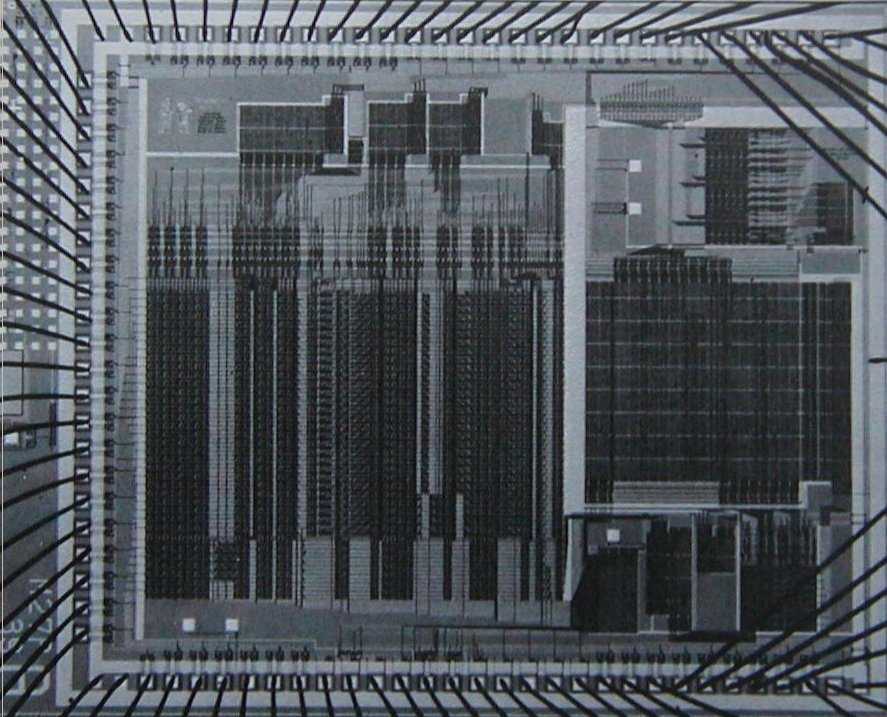
\includegraphics[width=91mm]{fig/chap5/chip.jpg}
\begin{quote}
\heading{Figure 5.16:} A silicon-chip implementation of an evaluator for Scheme.
\end{quote}
\end{figure}

\subsubsection*{Registers and operations}

In designing the explicit-control evaluator, we must specify the operations to
be used in our register machine.  We described the metacircular evaluator in
terms of abstract syntax, using procedures such as \code{quoted?} and
\code{make\-/procedure}.  In implementing the register machine, we could expand
these procedures into sequences of elementary list-structure memory operations,
and implement these operations on our register machine.  However, this would
make our evaluator very long, obscuring the basic structure with details.  To
clarify the presentation, we will include as primitive operations of the
register machine the syntax procedures given in \link{Section 4.1.2} and the
procedures for representing environments and other run-time data given in
sections \link{Section 4.1.3} and \link{Section 4.1.4}.  In order to completely specify an
evaluator that could be programmed in a low-level machine language or
implemented in hardware, we would replace these operations by more elementary
operations, using the list-structure implementation we described in
\link{Section 5.3}.

Our Scheme evaluator register machine includes a stack and seven registers:
\code{exp}, \code{env}, \code{val}, \code{continue}, \code{proc}, \code{argl},
and \code{unev}.  \code{exp} is used to hold the expression to be evaluated,
and \code{env} contains the environment in which the evaluation is to be
performed.  At the end of an evaluation, \code{val} contains the value obtained
by evaluating the expression in the designated environment.  The
\code{continue} register is used to implement recursion, as explained in
\link{Section 5.1.4}.  (The evaluator needs to call itself recursively, since
evaluating an expression requires evaluating its subexpressions.)  The
registers \code{proc}, \code{argl}, and \code{unev} are used in evaluating
combinations.

We will not provide a data-path diagram to show how the registers and
operations of the evaluator are connected, nor will we give the complete list
of machine operations.  These are implicit in the evaluator's controller, which
will be presented in detail.



\subsection{The Core of the Explicit-Control Evaluator}
\label{Section 5.4.1}

The central element in the evaluator is the sequence of instructions beginning
at \code{eval\-/dispatch}.  This corresponds to the \code{eval} procedure of the
metacircular evaluator described in \link{Section 4.1.1}.  When the controller
starts at \code{eval\-/dispatch}, it evaluates the expression specified by
\code{exp} in the environment specified by \code{env}.  When evaluation is
complete, the controller will go to the entry point stored in \code{continue},
and the \code{val} register will hold the value of the expression.  As with the
metacircular \code{eval}, the structure of \code{eval\-/dispatch} is a case
analysis on the syntactic type of the expression to be evaluated.\footnote{In
our controller, the dispatch is written as a sequence of \code{test} and
\code{branch} instructions.  Alternatively, it could have been written in a
data-directed style (and in a real system it probably would have been) to avoid
the need to perform sequential tests and to facilitate the definition of new
expression types.  A machine designed to run Lisp would probably include a
\code{dispatch\-/on\-/type} instruction that would efficiently execute such
data-directed dispatches.}

\begin{scheme}
eval-dispatch
  (test (op self-evaluating?) (reg exp))
  (branch (label ev-self-eval))
  (test (op variable?) (reg exp))
  (branch (label ev-variable))
  (test (op quoted?) (reg exp))
  (branch (label ev-quoted))
  (test (op assignment?) (reg exp))
  (branch (label ev-assignment))
  (test (op definition?) (reg exp))
  (branch (label ev-definition))
  (test (op if?) (reg exp))
  (branch (label ev-if))
  (test (op lambda?) (reg exp))
  (branch (label ev-lambda))
  (test (op begin?) (reg exp))
  (branch (label ev-begin))
  (test (op application?) (reg exp))
  (branch (label ev-application))
  (goto (label unknown-expression-type))
\end{scheme}

\subsubsection*{Evaluating simple expressions}

Numbers and strings (which are self-evaluating), variables, quotations, and
\code{lambda} expressions have no subexpressions to be evaluated.  For these,
the evaluator simply places the correct value in the \code{val} register and
continues execution at the entry point specified by \code{continue}.
Evaluation of simple expressions is performed by the following controller code:

\begin{scheme}
ev-self-eval
  (assign val (reg exp))
  (goto (reg continue))
ev-variable
  (assign val (op lookup-variable-value) (reg exp) (reg env))
  (goto (reg continue))
ev-quoted
  (assign val (op text-of-quotation) (reg exp))
  (goto (reg continue))
ev-lambda
  (assign unev (op lambda-parameters) (reg exp))
  (assign exp (op lambda-body) (reg exp))
  (assign val (op make-procedure) (reg unev) (reg exp) (reg env))
  (goto (reg continue))
\end{scheme}

\noindent
Observe how \code{ev\-/lambda} uses the \code{unev} and \code{exp} registers to
hold the parameters and body of the lambda expression so that they can be
passed to the \code{make\-/procedure} operation, along with the environment in
\code{env}.

\subsubsection*{Evaluating procedure applications}

A procedure application is specified by a combination containing an operator
and operands.  The operator is a subexpression whose value is a procedure, and
the operands are subexpressions whose values are the arguments to which the
procedure should be applied.  The metacircular \code{eval} handles applications
by calling itself recursively to evaluate each element of the combination, and
then passing the results to \code{apply}, which performs the actual procedure
application.  The explicit-control evaluator does the same thing; these
recursive calls are implemented by \code{goto} instructions, together with use
of the stack to save registers that will be restored after the recursive call
returns.  Before each call we will be careful to identify which registers must
be saved (because their values will be needed later).\footnote{This is an
important but subtle point in translating algorithms from a procedural
language, such as Lisp, to a register-machine language.  As an alternative to
saving only what is needed, we could save all the registers (except \code{val})
before each recursive call. This is called a \newterm{framed-stack} discipline.
This would work but might save more registers than necessary; this could be an
important consideration in a system where stack operations are expensive.
Saving registers whose contents will not be needed later may also hold onto
useless data that could otherwise be garbage-collected, freeing space to be
reused.}

We begin the evaluation of an application by evaluating the operator to produce
a procedure, which will later be applied to the evaluated operands.  To
evaluate the operator, we move it to the \code{exp} register and go to
\code{eval\-/dispatch}.  The environment in the \code{env} register is already
the correct one in which to evaluate the operator.  However, we save \code{env}
because we will need it later to evaluate the operands.  We also extract the
operands into \code{unev} and save this on the stack.  We set up
\code{continue} so that \code{eval\-/dispatch} will resume at
\code{ev\-/appl\-/did\-/operator} after the operator has been evaluated.  First,
however, we save the old value of \code{continue}, which tells the controller
where to continue after the application.

\enlargethispage{\baselineskip}

\begin{scheme}
ev-application
  (save continue)
  (save env)
  (assign unev (op operands) (reg exp))
  (save unev)
  (assign exp (op operator) (reg exp))
  (assign continue (label ev-appl-did-operator))
  (goto (label eval-dispatch))
\end{scheme}

\noindent
Upon returning from evaluating the operator subexpression, we proceed to
evaluate the operands of the combination and to accumulate the resulting
arguments in a list, held in \code{argl}.  First we restore the unevaluated
operands and the environment.  We initialize \code{argl} to an empty list.
Then we assign to the \code{proc} register the procedure that was produced by
evaluating the operator.  If there are no operands, we go directly to
\code{apply\-/dispatch}.  Otherwise we save \code{proc} on the stack and start
the argument-evaluation loop:\footnote{We add to the evaluator data-structure
procedures in \link{Section 4.1.3} the following two procedures for manipulating
argument lists:

\begin{smallscheme}
(define (empty-arglist) '())
(define (adjoin-arg arg arglist) (append arglist (list arg)))
\end{smallscheme}

We also use an additional syntax procedure to test for the last operand in a
combination:

\begin{smallscheme}
(define (last-operand? ops) (null? (cdr ops)))
\end{smallscheme} }

\begin{scheme}
ev-appl-did-operator
  (restore unev)                       ~\textrm{; the operands}~
  (restore env)
  (assign argl (op empty-arglist))
  (assign proc (reg val))              ~\textrm{; the operator}~
  (test (op no-operands?) (reg unev))
  (branch (label apply-dispatch))
  (save proc)
\end{scheme}

\noindent
Each cycle of the argument-evaluation loop evaluates an operand from the list
in \code{unev} and accumulates the result into \code{argl}.  To evaluate an
operand, we place it in the \code{exp} register and go to \code{eval\-/dispatch},
after setting \code{continue} so that execution will resume with the
argument-accumulation phase.  But first we save the arguments accumulated so
far (held in \code{argl}), the environment (held in \code{env}), and the
remaining operands to be evaluated (held in \code{unev}).  A special case is
made for the evaluation of the last operand, which is handled at
\code{ev\-/appl\-/last\-/arg}.

\begin{scheme}
ev-appl-operand-loop
  (save argl)
  (assign exp (op first-operand) (reg unev))
  (test (op last-operand?) (reg unev))
  (branch (label ev-appl-last-arg))
  (save env)
  (save unev)
  (assign continue (label ev-appl-accumulate-arg))
  (goto (label eval-dispatch))
\end{scheme}

\noindent
When an operand has been evaluated, the value is accumulated into the list held
in \code{argl}.  The operand is then removed from the list of unevaluated
operands in \code{unev}, and the argument-evaluation continues.

\begin{scheme}
ev-appl-accumulate-arg
  (restore unev)
  (restore env)
  (restore argl)
  (assign argl (op adjoin-arg) (reg val) (reg argl))
  (assign unev (op rest-operands) (reg unev))
  (goto (label ev-appl-operand-loop))
\end{scheme}

\noindent
Evaluation of the last argument is handled differently.  There is no need to
save the environment or the list of unevaluated operands before going to
\code{eval\-/dispatch}, since they will not be required after the last operand is
evaluated.  Thus, we return from the evaluation to a special entry point
\code{ev\-/appl\-/accum\-/last\-/arg}, which restores the argument list, accumulates
the new argument, restores the saved procedure, and goes off to perform the
application.\footnote{The optimization of treating the last operand specially
is known as \newterm{evlis tail recursion} (see \link{Wand 1980}).  We could be
somewhat more efficient in the argument evaluation loop if we made evaluation
of the first operand a special case too.  This would permit us to postpone
initializing \code{argl} until after evaluating the first operand, so as to
avoid saving \code{argl} in this case.  The compiler in \link{Section 5.5}
performs this optimization.  (Compare the \code{construct\-/arglist} procedure of
\link{Section 5.5.3}.)}

\begin{scheme}
ev-appl-last-arg
  (assign continue (label ev-appl-accum-last-arg))
  (goto (label eval-dispatch))
ev-appl-accum-last-arg
  (restore argl)
  (assign argl (op adjoin-arg) (reg val) (reg argl))
  (restore proc)
  (goto (label apply-dispatch))
\end{scheme}

\noindent
The details of the argument-evaluation loop determine the order in which the
interpreter evaluates the operands of a combination (e.g., left to right or
right to left---see \link{Exercise 3.8}).  This order is not determined by the
metacircular evaluator, which inherits its control structure from the
underlying Scheme in which it is implemented.\footnote{The order of operand
evaluation in the metacircular evaluator is determined by the order of
evaluation of the arguments to \code{cons} in the procedure
\code{list\-/of\-/values} of \link{Section 4.1.1} (see \link{Exercise 4.1}).} Because
the \code{first\-/operand} selector (used in \code{ev\-/appl\-/operand\-/loop} to
extract successive operands from \code{unev}) is implemented as \code{car} and
the \code{rest\-/operands} selector is implemented as \code{cdr}, the
explicit-control evaluator will evaluate the operands of a combination in
left-to-right order.

\subsubsection*{Procedure application}

The entry point \code{apply\-/dispatch} corresponds to the \code{apply} procedure
of the metacircular evaluator.  By the time we get to \code{apply\-/dispatch},
the \code{proc} register contains the procedure to apply and \code{argl}
contains the list of evaluated arguments to which it must be applied.  The
saved value of \code{continue} (originally passed to \code{eval\-/dispatch} and
saved at \code{ev\-/application}), which tells where to return with the result of
the procedure application, is on the stack.  When the application is complete,
the controller transfers to the entry point specified by the saved
\code{continue}, with the result of the application in \code{val}.  As with the
metacircular \code{apply}, there are two cases to consider.  Either the
procedure to be applied is a primitive or it is a compound procedure.

\begin{scheme}
apply-dispatch
  (test (op primitive-procedure?) (reg proc))
  (branch (label primitive-apply))
  (test (op compound-procedure?) (reg proc))
  (branch (label compound-apply))
  (goto (label unknown-procedure-type))
\end{scheme}

\noindent
We assume that each primitive is implemented so as to obtain its arguments from
\code{argl} and place its result in \code{val}.  To specify how the machine
handles primitives, we would have to provide a sequence of controller
instructions to implement each primitive and arrange for \code{primitive\-/apply}
to dispatch to the instructions for the primitive identified by the contents of
\code{proc}.  Since we are interested in the structure of the evaluation
process rather than the details of the primitives, we will instead just use an
\code{apply\-/primitive\-/procedure} operation that applies the procedure in
\code{proc} to the arguments in \code{argl}.  For the purpose of simulating the
evaluator with the simulator of \link{Section 5.2} we use the procedure
\code{apply\-/primitive\-/procedure}, which calls on the underlying Scheme system
to perform the application, just as we did for the metacircular evaluator in
\link{Section 4.1.4}.  After computing the value of the primitive application,
we restore \code{continue} and go to the designated entry point.

\begin{scheme}

primitive-apply
  (assign val (op apply-primitive-procedure)
              (reg proc)
              (reg argl))
  (restore continue)
  (goto (reg continue))
\end{scheme}

\noindent
To apply a compound procedure, we proceed just as with the metacircular
evaluator.  We construct a frame that binds the procedure's parameters to the
arguments, use this frame to extend the environment carried by the procedure,
and evaluate in this extended environment the sequence of expressions that
forms the body of the procedure.  \code{ev\-/sequence}, described below in
\link{Section 5.4.2}, handles the evaluation of the sequence.

\begin{scheme}
compound-apply
  (assign unev (op procedure-parameters) (reg proc))
  (assign env (op procedure-environment) (reg proc))
  (assign env (op extend-environment)
              (reg unev) (reg argl) (reg env))
  (assign unev (op procedure-body) (reg proc))
  (goto (label ev-sequence))
\end{scheme}

\noindent
\code{compound\-/apply} is the only place in the interpreter where the \code{env}
register is ever assigned a new value.  Just as in the metacircular evaluator,
the new environment is constructed from the environment carried by the
procedure, together with the argument list and the corresponding list of
variables to be bound.

\subsection{Sequence Evaluation and Tail Recursion}
\label{Section 5.4.2}

The portion of the explicit-control evaluator at \code{ev\-/sequence} is
analogous to the metacircular evaluator's \code{eval\-/sequence} procedure.  It
handles sequences of expressions in procedure bodies or in explicit
\code{begin} expressions.

Explicit \code{begin} expressions are evaluated by placing the sequence of
expressions to be evaluated in \code{unev}, saving \code{continue} on the
stack, and jumping to \code{ev\-/sequence}.

\begin{scheme}
ev-begin
  (assign unev (op begin-actions) (reg exp))
  (save continue)
  (goto (label ev-sequence))
\end{scheme}

\noindent
The implicit sequences in procedure bodies are handled by jumping to
\code{ev\-/sequence} from \code{compound\-/apply}, at which point \code{continue}
is already on the stack, having been saved at \code{ev\-/application}.

The entries at \code{ev\-/sequence} and \code{ev\-/sequence\-/continue} form a loop
that successively evaluates each expression in a sequence.  The list of
unevaluated expressions is kept in \code{unev}.  Before evaluating each
expression, we check to see if there are additional expressions to be evaluated
in the sequence.  If so, we save the rest of the unevaluated expressions (held
in \code{unev}) and the environment in which these must be evaluated (held in
\code{env}) and call \code{eval\-/dispatch} to evaluate the expression.  The two
saved registers are restored upon the return from this evaluation, at
\code{ev\-/sequence\-/continue}.

The final expression in the sequence is handled differently, at the entry point
\code{ev\-/sequence\-/last\-/exp}.  Since there are no more expressions to be
evaluated after this one, we need not save \code{unev} or \code{env} before
going to \code{eval\-/dispatch}.  The value of the whole sequence is the value of
the last expression, so after the evaluation of the last expression there is
nothing left to do except continue at the entry point currently held on the
stack (which was saved by \code{ev\-/application} or \code{ev\-/begin}.)  Rather
than setting up \code{continue} to arrange for \code{eval\-/dispatch} to return
here and then restoring \code{continue} from the stack and continuing at that
entry point, we restore \code{continue} from the stack before going to
\code{eval\-/dispatch}, so that \code{eval\-/dispatch} will continue at that entry
point after evaluating the expression.

\begin{scheme}
ev-sequence
  (assign exp (op first-exp) (reg unev))
  (test (op last-exp?) (reg unev))
  (branch (label ev-sequence-last-exp))
  (save unev)
  (save env)
  (assign continue (label ev-sequence-continue))
  (goto (label eval-dispatch))
ev-sequence-continue
  (restore env)
  (restore unev)
  (assign unev (op rest-exps) (reg unev))
  (goto (label ev-sequence))
ev-sequence-last-exp
  (restore continue)
  (goto (label eval-dispatch))
\end{scheme}

\subsubsection*{Tail recursion}

In \link{Chapter 1} we said that the process described by a procedure such as

\begin{scheme}
(define (sqrt-iter guess x)
  (if (good-enough? guess x)
      guess
      (sqrt-iter (improve guess x) x)))
\end{scheme}

\noindent
is an iterative process.  Even though the procedure is syntactically recursive
(defined in terms of itself), it is not logically necessary for an evaluator to
save information in passing from one call to \code{sqrt\-/iter} to the
next.\footnote{We saw in \link{Section 5.1} how to implement such a process with
a register machine that had no stack; the state of the process was stored in a
fixed set of registers.} An evaluator that can execute a procedure such as
\code{sqrt\-/iter} without requiring increasing storage as the procedure
continues to call itself is called a \newterm{tail-recursive} evaluator.  The
metacircular implementation of the evaluator in \link{Chapter 4} does not
specify whether the evaluator is tail-recursive, because that evaluator
inherits its mechanism for saving state from the underlying Scheme.  With the
explicit-control evaluator, however, we can trace through the evaluation
process to see when procedure calls cause a net accumulation of information on
the stack.

Our evaluator is tail-recursive, because in order to evaluate the final
expression of a sequence we transfer directly to \code{eval\-/dispatch} without
saving any information on the stack.  Hence, evaluating the final expression in
a sequence---even if it is a procedure call (as in \code{sqrt\-/iter}, where the
\code{if} expression, which is the last expression in the procedure body,
reduces to a call to \code{sqrt\-/iter})---will not cause any information to be
accumulated on the stack.\footnote{This implementation of tail recursion in
\code{ev\-/sequence} is one variety of a well-known optimization technique used
by many compilers.  In compiling a procedure that ends with a procedure call,
one can replace the call by a jump to the called procedure's entry point.
Building this strategy into the interpreter, as we have done in this section,
provides the optimization uniformly throughout the language.}

\enlargethispage{\baselineskip}

If we did not think to take advantage of the fact that it was unnecessary to
save information in this case, we might have implemented \code{eval\-/sequence}
by treating all the expressions in a sequence in the same way---saving the
registers, evaluating the expression, returning to restore the registers, and
repeating this until all the expressions have been evaluated:\footnote{We can
define \code{no\-/more\-/exps?} as follows:

\begin{smallscheme}
(define (no-more-exps? seq) (null? seq))
\end{smallscheme}
}

\begin{scheme}
ev-sequence
  (test (op no-more-exps?) (reg unev))
  (branch (label ev-sequence-end))
  (assign exp (op first-exp) (reg unev))
  (save unev)
  (save env)
  (assign continue (label ev-sequence-continue))
  (goto (label eval-dispatch))
ev-sequence-continue
  (restore env)
  (restore unev)
  (assign unev (op rest-exps) (reg unev))
  (goto (label ev-sequence))
ev-sequence-end
  (restore continue)
  (goto (reg continue))
\end{scheme}

\enlargethispage{\baselineskip}

\noindent
This may seem like a minor change to our previous code for evaluation of a
sequence: The only difference is that we go through the save-restore cycle for
the last expression in a sequence as well as for the others.  The interpreter
will still give the same value for any expression.  But this change is fatal to
the tail-recursive implementation, because we must now return after evaluating
the final expression in a sequence in order to undo the (useless) register
saves.  These extra saves will accumulate during a nest of procedure calls.
Consequently, processes such as \code{sqrt\-/iter} will require space
proportional to the number of iterations rather than requiring constant space.
This difference can be significant.  For example, with tail recursion, an
infinite loop can be expressed using only the procedure-call mechanism:

\begin{scheme}
(define (count n)
  (newline) (display n) (count (+ n 1)))
\end{scheme}

\noindent
Without tail recursion, such a procedure would eventually run out of stack
space, and expressing a true iteration would require some control mechanism
other than procedure call.

\subsection{Conditionals, Assignments, and Definitions}
\label{Section 5.4.3}

As with the metacircular evaluator, special forms are handled by selectively
evaluating fragments of the expression.  For an \code{if} expression, we must
evaluate the predicate and decide, based on the value of predicate, whether to
evaluate the consequent or the alternative.

Before evaluating the predicate, we save the \code{if} expression itself so
that we can later extract the consequent or alternative.  We also save the
environment, which we will need later in order to evaluate the consequent or
the alternative, and we save \code{continue}, which we will need later in order
to return to the evaluation of the expression that is waiting for the value of
the \code{if}.

\begin{scheme}
ev-if
  (save exp)                    ~\textrm{; save expression for later}~
  (save env)
  (save continue)
  (assign continue (label ev-if-decide))
  (assign exp (op if-predicate) (reg exp))
  (goto (label eval-dispatch))  ~\textrm{; evaluate the predicate}~
\end{scheme}

\noindent
When we return from evaluating the predicate, we test whether it was true or
false and, depending on the result, place either the consequent or the
alternative in \code{exp} before going to \code{eval\-/dispatch}.  Notice that
restoring \code{env} and \code{continue} here sets up \code{eval\-/dispatch} to
have the correct environment and to continue at the right place to receive the
value of the \code{if} expression.

\begin{scheme}

ev-if-decide
  (restore continue)
  (restore env)
  (restore exp)
  (test (op true?) (reg val))
  (branch (label ev-if-consequent))
ev-if-alternative
  (assign exp (op if-alternative) (reg exp))
  (goto (label eval-dispatch))
ev-if-consequent
  (assign exp (op if-consequent) (reg exp))
  (goto (label eval-dispatch))
\end{scheme}

\enlargethispage{\baselineskip}

\subsubsection*{Assignments and definitions}

Assignments are handled by \code{ev\-/assignment}, which is reached from
\code{eval\-/dispatch} with the assignment expression in \code{exp}.  The code at
\code{ev\-/assignment} first evaluates the value part of the expression and then
installs the new value in the environment.  \code{set\-/variable\-/value!} is
assumed to be available as a machine operation.

\begin{scheme}
ev-assignment
  (assign unev (op assignment-variable) (reg exp))
  (save unev)                   ~\textrm{; save variable for later}~
  (assign exp (op assignment-value) (reg exp))
  (save env)
  (save continue)
  (assign continue (label ev-assignment-1))
  (goto (label eval-dispatch))  ~\textrm{; evaluate the assignment value}~
ev-assignment-1
  (restore continue)
  (restore env)
  (restore unev)
  (perform
   (op set-variable-value!) (reg unev) (reg val) (reg env))
  (assign val (const ok))
  (goto (reg continue))
\end{scheme}

\noindent
Definitions are handled in a similar way:

\begin{scheme}
ev-definition
  (assign unev (op definition-variable) (reg exp))
  (save unev)                   ~\textrm{; save variable for later}~
  (assign exp (op definition-value) (reg exp))
  (save env)
  (save continue)
  (assign continue (label ev-definition-1))
  (goto (label eval-dispatch))  ~\textrm{; evaluate the definition value}~
ev-definition-1
  (restore continue)
  (restore env)
  (restore unev)
  (perform
   (op define-variable!) (reg unev) (reg val) (reg env))
  (assign val (const ok))
  (goto (reg continue))
\end{scheme}

\begin{quote}
\heading{\phantomsection\label{Exercise 5.23}Exercise 5.23:} Extend the evaluator to handle
derived expressions such as \code{cond}, \code{let}, and so on
(\link{Section 4.1.2}).  You may ``cheat'' and assume that the syntax transformers such
as \code{cond\-/>if} are available as machine operations.\footnote{This isn't
really cheating.  In an actual implementation built from scratch, we would use
our explicit-control evaluator to interpret a Scheme program that performs
source-level transformations like \code{cond\-/>if} in a syntax phase that runs
before execution.}
\end{quote}

\begin{quote}
\heading{\phantomsection\label{Exercise 5.24}Exercise 5.24:} Implement \code{cond} as a new
basic special form without reducing it to \code{if}.  You will have to
construct a loop that tests the predicates of successive \code{cond} clauses
until you find one that is true, and then use \code{ev\-/sequence} to evaluate
the actions of the clause.
\end{quote}

\begin{quote}
\heading{\phantomsection\label{Exercise 5.25}Exercise 5.25:} Modify the evaluator so that it
uses normal-order evaluation, based on the lazy evaluator of \link{Section 4.2}.
\end{quote}

\subsection{Running the Evaluator}
\label{Section 5.4.4}

With the implementation of the explicit-control evaluator we come to the end of
a development, begun in \link{Chapter 1}, in which we have explored successively
more precise models of the evaluation process.  We started with the relatively
informal substitution model, then extended this in \link{Chapter 3} to the
environment model, which enabled us to deal with state and change.  In the
metacircular evaluator of \link{Chapter 4}, we used Scheme itself as a language
for making more explicit the environment structure constructed during
evaluation of an expression.  Now, with register machines, we have taken a
close look at the evaluator's mechanisms for storage management, argument
passing, and control.  At each new level of description, we have had to raise
issues and resolve ambiguities that were not apparent at the previous, less
precise treatment of evaluation.  To understand the behavior of the
explicit-control evaluator, we can simulate it and monitor its performance.

We will install a driver loop in our evaluator machine.  This plays the role of
the \code{driver\-/loop} procedure of \link{Section 4.1.4}.  The evaluator will
repeatedly print a prompt, read an expression, evaluate the expression by going
to \code{eval\-/dispatch}, and print the result.  The following instructions form
the beginning of the explicit-control evaluator's controller
sequence:\footnote{We assume here that \code{read} and the various printing
operations are available as primitive machine operations, which is useful for
our simulation, but completely unrealistic in practice.  These are actually
extremely complex operations.  In practice, they would be implemented using
low-level input-output operations such as transferring single characters to and
from a device.

To support the \code{get\-/global\-/environment} operation we define

\begin{smallscheme}
(define the-global-environment (setup-environment))
(define (get-global-environment) the-global-environment)
\end{smallscheme}
}

\begin{scheme}
read-eval-print-loop
  (perform (op initialize-stack))
  (perform
   (op prompt-for-input) (const ";;EC-Eval input:"))
  (assign exp (op read))
  (assign env (op get-global-environment))
  (assign continue (label print-result))
  (goto (label eval-dispatch))
print-result
  (perform (op announce-output) (const ";;EC-Eval value:"))
  (perform (op user-print) (reg val))
  (goto (label read-eval-print-loop))
\end{scheme}

\noindent
When we encounter an error in a procedure (such as the ``unknown procedure type
error'' indicated at \code{apply\-/dispatch}), we print an error message and
return to the driver loop.\footnote{There are other errors that we would like
the interpreter to handle, but these are not so simple.  See \link{Exercise 5.30}.}

\begin{scheme}
unknown-expression-type
  (assign val (const unknown-expression-type-error))
  (goto (label signal-error))
unknown-procedure-type
  (restore continue)    ~\textrm{; clean up stack (from \code{apply\-/dispatch})}~
  (assign val (const unknown-procedure-type-error))
  (goto (label signal-error))
signal-error
  (perform (op user-print) (reg val))
  (goto (label read-eval-print-loop))
\end{scheme}

\noindent
For the purposes of the simulation, we initialize the stack each time through
the driver loop, since it might not be empty after an error (such as an
undefined variable) interrupts an evaluation.\footnote{We could perform the
stack initialization only after errors, but doing it in the driver loop will be
convenient for monitoring the evaluator's performance, as described below.}

If we combine all the code fragments presented in
\link{Section 5.4.1}--\link{Section 5.4.4}, we can create an evaluator machine model that we can
run using the register-machine simulator of \link{Section 5.2}.

\begin{scheme}
(define eceval
  (make-machine
   '(exp env val proc argl continue unev)
   eceval-operations
   '(read-eval-print-loop
     ~\( \dark \langle \)~~\emph{entire machine controller as given above}~~\( \dark \rangle \)~ )))
\end{scheme}

\noindent
We must define Scheme procedures to simulate the operations used as primitives
by the evaluator.  These are the same procedures we used for the metacircular
evaluator in \link{Section 4.1}, together with the few additional ones defined
in footnotes throughout \link{Section 5.4}.

\begin{scheme}
(define eceval-operations
  (list (list 'self-evaluating? self-evaluating)
        ~\( \dark \langle \)~~\emph{complete list of operations for eceval machine}~~\( \dark \rangle \)~))
\end{scheme}

\noindent
Finally, we can initialize the global environment and run the evaluator:

\begin{scheme}
(define the-global-environment (setup-environment))
(start eceval)
~\textit{;;; EC-Eval input:}~
(define (append x y)
  (if (null? x) y (cons (car x) (append (cdr x) y))))
~\textit{;;; EC-Eval value:}~
~\textit{ok}~
~\textit{;;; EC-Eval input:}~
(append '(a b c) '(d e f))
~\textit{;;; EC-Eval value:}~
~\textit{(a b c d e f)}~
\end{scheme}

\noindent
Of course, evaluating expressions in this way will take much longer than if we
had directly typed them into Scheme, because of the multiple levels of
simulation involved.  Our expressions are evaluated by the
explicit-control-evaluator machine, which is being simulated by a Scheme
program, which is itself being evaluated by the Scheme interpreter.

\subsubsection*{Monitoring the performance of the evaluator}

Simulation can be a powerful tool to guide the implementation of evaluators.
Simulations make it easy not only to explore variations of the register-machine
design but also to monitor the performance of the simulated evaluator.  For
example, one important factor in performance is how efficiently the evaluator
uses the stack.  We can observe the number of stack operations required to
evaluate various expressions by defining the evaluator register machine with
the version of the simulator that collects statistics on stack use
(\link{Section 5.2.4}), and adding an instruction at the evaluator's \code{print\-/result}
entry point to print the statistics:

\begin{scheme}
print-result
  (perform (op print-stack-statistics))   ~\textrm{; added instruction}~
  (perform
   (op announce-output) (const ";;; EC-Eval value:"))
  ~\( \dots \)~ ~\textrm{; same as before}~
\end{scheme}

\noindent
Interactions with the evaluator now look like this:

\begin{scheme}
~\textit{;;; EC-Eval input:}~
(define (factorial n)
  (if (= n 1) 1 (* (factorial (- n 1)) n)))
~\textit{(total-pushes = 3 maximum-depth = 3)}~
~\textit{;;; EC-Eval value:}~
~\textit{ok}~
~\textit{;;; EC-Eval input:}~
(factorial 5)
~\textit{(total-pushes = 144 maximum-depth = 28)}~
~\textit{;;; EC-Eval value:}~
~\textit{120}~
\end{scheme}

\noindent
Note that the driver loop of the evaluator reinitializes the stack at the start
of each interaction, so that the statistics printed will refer only to stack
operations used to evaluate the previous expression.

\begin{quote}
\heading{\phantomsection\label{Exercise 5.26}Exercise 5.26:} Use the monitored stack to
explore the tail-recursive property of the evaluator (\link{Section 5.4.2}).
Start the evaluator and define the iterative \code{factorial} procedure from
\link{Section 1.2.1}:

\begin{scheme}
(define (factorial n)
  (define (iter product counter)
    (if (> counter n)
        product
        (iter (* counter product) (+ counter 1))))
  (iter 1 1))
\end{scheme}

Run the procedure with some small values of \( n \).  Record the maximum stack
depth and the number of pushes required to compute \( n! \) for each of these
values.

\begin{enumerate}[a.]

\item
You will find that the maximum depth required to evaluate \( n! \) is independent
of \( n \).  What is that depth?

\item
Determine from your data a formula in terms of \( n \) for the total number of
push operations used in evaluating \( n! \) for any \( n \ge 1 \).  Note that the
number of operations used is a linear function of \( n \) and is thus determined
by two constants.

\end{enumerate}
\end{quote}

\begin{quote}
\heading{\phantomsection\label{Exercise 5.27}Exercise 5.27:} For comparison with \link{Exercise 5.26},
explore the behavior of the following procedure for computing factorials
recursively:

\begin{scheme}
(define (factorial n)
  (if (= n 1) 1 (* (factorial (- n 1)) n)))
\end{scheme}

By running this procedure with the monitored stack, determine, as a function of
\( n \), the maximum depth of the stack and the total number of pushes used in
evaluating \( n! \) for \( n \ge 1 \).  (Again, these functions will be linear.)
Summarize your experiments by filling in the following table with the
appropriate expressions in terms of \( n \):
\begin{comment}

\begin{example}
               Maximum depth       Number of pushes

Recursive
factorial

Iterative
factorial
\end{example}

\end{comment}

$$\vbox{
\offinterlineskip
\halign{
\strut 	\hfil \quad #\quad \hfil & \vrule
	\hfil \quad #\quad \hfil & \vrule
	\hfil \quad #\quad \hfil \cr

				& Maximum depth & Number of pushes \cr
	\noalign{\hrule}
	Recursive 		&  		&  \cr
	factorial 		&  		&  \cr
	\noalign{\hrule}
	Iterative 		&  		&  \cr
	factorial 		&  		&  \cr
}
}$$

The maximum depth is a measure of the amount of space used by the evaluator in
carrying out the computation, and the number of pushes correlates well with the
time required.
\end{quote}

\begin{quote}
\heading{\phantomsection\label{Exercise 5.28}Exercise 5.28:} Modify the definition of the
evaluator by changing \code{eval\-/sequence} as described in \link{Section 5.4.2}
so that the evaluator is no longer tail-recursive.  Rerun your experiments from
\link{Exercise 5.26} and \link{Exercise 5.27} to demonstrate that both versions
of the \code{factorial} procedure now require space that grows linearly with
their input.
\end{quote}

\begin{quote}
\heading{\phantomsection\label{Exercise 5.29}Exercise 5.29:} Monitor the stack operations in
the tree-recursive Fibonacci computation:

\begin{scheme}
(define (fib n)
  (if (< n 2)
      n
      (+ (fib (- n 1)) (fib (- n 2)))))
\end{scheme}

\begin{enumerate}[a.]

\item
Give a formula in terms of \( n \) for the maximum depth of the stack required to
compute \( {\rm Fib}(n) \) for \( n \ge 2 \).  Hint: In \link{Section 1.2.2} we
argued that the space used by this process grows linearly with \( n \).

\item
Give a formula for the total number of pushes used to compute \( {\rm Fib}(n) \)
for \( n \ge 2 \).  You should find that the number of pushes (which correlates
well with the time used) grows exponentially with \( n \).  Hint: Let
\( S(n) \) be the number of pushes used in computing \( {\rm Fib}(n) \).  You
should be able to argue that there is a formula that expresses \( S(n) \) in
terms of \( S(n - 1) \), \( S(n - 2) \), and some fixed ``overhead''
constant \( k \) that is independent of \( n \).  Give the formula, and say what
\( k \) is.  Then show that \( S(n) \) can be expressed as
\( a\cdot{\rm Fib}(n + 1) + b \) and give the values of \( a \) and \( b \).

\end{enumerate}
\end{quote}

\begin{quote}
\heading{\phantomsection\label{Exercise 5.30}Exercise 5.30:} Our evaluator currently catches
and signals only two kinds of errors---unknown expression types and unknown
procedure types.  Other errors will take us out of the evaluator
read-eval-print loop.  When we run the evaluator using the register-machine
simulator, these errors are caught by the underlying Scheme system.  This is
analogous to the computer crashing when a user program makes an
error.\footnote{Regrettably, this is the normal state of affairs in
conventional compiler-based language systems such as C.  In \acronym{UNIX}(tm)
the system ``dumps core,'' and in \acronym{DOS}/Windows(tm) it becomes
catatonic.  The Macintosh(tm) displays a picture of an exploding bomb and
offers you the opportunity to reboot the computer---if you're lucky.}  It is a
large project to make a real error system work, but it is well worth the effort
to understand what is involved here.

\begin{enumerate}[a.]

\item
Errors that occur in the evaluation process, such as an attempt to access an
unbound variable, could be caught by changing the lookup operation to make it
return a distinguished condition code, which cannot be a possible value of any
user variable.  The evaluator can test for this condition code and then do what
is necessary to go to \code{signal\-/error}.  Find all of the places in the
evaluator where such a change is necessary and fix them.  This is lots of work.

\item
Much worse is the problem of handling errors that are signaled by applying
primitive procedures, such as an attempt to divide by zero or an attempt to
extract the \code{car} of a symbol.  In a professionally written high-quality
system, each primitive application is checked for safety as part of the
primitive.  For example, every call to \code{car} could first check that the
argument is a pair.  If the argument is not a pair, the application would
return a distinguished condition code to the evaluator, which would then report
the failure.  We could arrange for this in our register-machine simulator by
making each primitive procedure check for applicability and returning an
appropriate distinguished condition code on failure. Then the
\code{primitive\-/apply} code in the evaluator can check for the condition code
and go to \code{signal\-/error} if necessary.  Build this structure and make it
work.  This is a major project.

\end{enumerate}
\end{quote}

\section{Compilation}
\label{Section 5.5}

The explicit-control evaluator of \link{Section 5.4} is a register machine whose controller interprets Scheme programs.
In this section we will see how to run Scheme programs on a register machine whose controller is not a Scheme interpreter.

The explicit-control evaluator machine is universal---it can carry out any computational process that can be described in Scheme.
The evaluator’s controller orchestrates the use of its data paths to perform the desired computation.
Thus, the evaluator’s data paths are universal:
They are sufficient to perform any computation we desire, given an appropriate controller.%
\footnote{%
	This is a theoretical statement.
	We are not claiming that the evaluator’s data paths are a particularly convenient or efficient set of data paths for a general-purpose computer.
	For example, they are not very good for implementing high-performance floating-point calculations or calculations that intensively manipulate bit vectors.
}

Commercial general-purpose computers are register machines organized around a collection of registers and operations that constitute an efficient and convenient universal set of data paths.
The controller for a general-purpose machine is an interpreter for a register-machine language like the one we have been using.
This language is called the \newterm{native language} of the machine, or simply \newterm{machine language}.
Programs written in machine language are sequences of instructions that use the machine’s data paths.
For example, the explicit-control evaluator’s instruction sequence can be thought of as a machine-language program for a general-purpose computer rather than as the controller for a specialized interpreter machine.

There are two common strategies for bridging the gap between higher-level languages and register-machine languages.
The explicit-control evaluator illustrates the strategy of interpretation.
An interpreter written in the native language of a machine configures the machine to execute programs written in a language (called the \newterm{source language}) that may differ from the native language of the machine performing the evaluation.
The primitive procedures of the source language are implemented as a library of subroutines written in the native language of the given machine.
A program to be interpreted (called the \newterm{source program}) is represented as a data structure.
The interpreter traverses this data structure, analyzing the source program.
As it does so, it simulates the intended behavior of the source program by calling appropriate primitive subroutines from the library.

In this section, we explore the alternative strategy of \newterm{compilation}.
A compiler for a given source language and machine translates a source program into an equivalent program (called the \newterm{object program}) written in the machine’s native language.
The compiler that we implement in this section translates programs written in Scheme into sequences of instructions to be executed using the explicit-control evaluator machine’s data paths.%
\footnote{
	Actually, the machine that runs compiled code can be simpler than the interpreter machine, because we won’t use the \code{exp} and \code{unev} registers.
	The interpreter used these to hold pieces of unevaluated expressions.
	With the compiler, however, these expressions get built into the compiled code that the register machine will run.
	For the same reason, we don’t need the machine operations that deal with expression syntax.
	But compiled code will use a few additional machine operations (to represent compiled procedure objects) that didn’t appear in the explicit-control evaluator machine.
}

Compared with interpretation, compilation can provide a great increase in the efficiency of program execution, as we will explain below in the overview of the compiler.
On the other hand, an interpreter provides a more powerful environment for interactive program development and debugging, because the source program being executed is available at run time to be examined and modified.
In addition, because the entire library of primitives is present, new programs can be constructed and added to the system during debugging.

In view of the complementary advantages of compilation and interpretation, modern program-development environments pursue a mixed strategy.
Lisp interpreters are generally organized so that interpreted procedures and compiled procedures can call each other.
This enables a programmer to compile those parts of a program that are assumed to be debugged, thus gaining the efficiency advantage of compilation, while retaining the interpretive mode of execution for those parts of the program that are in the flux of interactive development and debugging.
In \link{Section 5.5.7}, after we have implemented the compiler, we will show how to interface it with our interpreter to produce an integrated interpreter-compiler development system.



\subsubsection*{An overview of the compiler}

Our compiler is much like our interpreter, both in its structure and in the function it performs.
Accordingly, the mechanisms used by the compiler for analyzing expressions will be similar to those used by the interpreter.
Moreover, to make it easy to interface compiled and interpreted code, we will design the compiler to generate code that obeys the same conventions of register usage as the interpreter:
The environment will be kept in the \code{env} register, argument lists will be accumulated in \code{argl}, a procedure to be applied will be in \code{proc}, procedures will return their answers in \code{val}, and the location to which a procedure should return will be kept in \code{continue}.
In general, the compiler translates a source program into an object program that performs essentially the same register operations as would the interpreter in evaluating the same source program.

This description suggests a strategy for implementing a rudimentary compiler:
We traverse the expression in the same way the interpreter does.
When we encounter a register instruction that the interpreter would perform in evaluating the expression, we do not execute the instruction but instead accumulate it into a sequence.
The resulting sequence of instructions will be the object code.
Observe the efficiency advantage of compilation over interpretation.
Each time the interpreter evaluates an expression---for example, \code{(f 84 96)}---it performs the work of classifying the expression (discovering that this is a procedure application) and testing for the end of the operand list (discovering that there are two operands).
With a compiler, the expression is analyzed only once, when the instruction sequence is generated at compile time.
The object code produced by the compiler contains only the instructions that evaluate the operator and the two operands, assemble the argument list, and apply the procedure (in \code{proc}) to the arguments (in \code{argl}).

This is the same kind of optimization we implemented in the analyzing evaluator of \link{Section 4.1.7}.
But there are further opportunities to gain efficiency in compiled code.
As the interpreter runs, it follows a process that must be applicable to any expression in the language.
In contrast, a given segment of compiled code is meant to execute some particular expression.
This can make a big difference, for example in the use of the stack to save registers.
When the interpreter evaluates an expression, it must be prepared for any contingency.
Before evaluating a subexpression, the interpreter saves all registers that will be needed later, because the subexpression might require an arbitrary evaluation.
A compiler, on the other hand, can exploit the structure of the particular expression it is processing to generate code that avoids unnecessary stack operations.

As a case in point, consider the combination \code{(f 84 96)}.
Before the interpreter evaluates the operator of the combination, it prepares for this evaluation by saving the registers containing the operands and the environment, whose values will be needed later.
The interpreter then evaluates the operator to obtain the result in \code{val}, restores the saved registers, and finally moves the result from \code{val} to \code{proc}.
However, in the particular expression we are dealing with, the operator is the symbol \code{f}, whose evaluation is accomplished by the machine operation \code{lookup-variable-value}, which does not alter any registers.
The compiler that we implement in this section will take advantage of this fact and generate code that evaluates the operator using the instruction
\begin{scheme}
  (assign proc (op lookup-variable-value)
               (const f)
               (reg env))
\end{scheme}
This code not only avoids the unnecessary saves and restores but also assigns the value of the lookup directly to \code{proc}, whereas the interpreter would obtain the result in \code{val} and then move this to \code{proc}.

A compiler can also optimize access to the environment.
Having analyzed the code, the compiler can in many cases know in which frame a particular variable will be located and access that frame directly, rather than performing the \code{lookup-variable-value} search.
We will discuss how to implement such variable access in \link{Section 5.5.6}.
Until then, however, we will focus on the kind of register and stack optimizations described above.
There are many other optimizations that can be performed by a compiler, such as coding primitive operations “in line” instead of using a general \code{apply} mechanism (see \link{Exercise 5.38});
but we will not emphasize these here.
Our main goal in this section is to illustrate the compilation process in a simplified (but still interesting) context.

\subsection{Structure of the Compiler}
\label{Section 5.5.1}

In \cref{Section 4.1.7} we modified our original metacircular interpreter to separate analysis from execution.
We analyzed each expression to produce an execution procedure that took an environment as argument and performed the required operations.
In our compiler, we will do essentially the same analysis.
Instead of producing execution procedures, however, we will generate sequences of instructions to be run by our register machine.

The procedure \code{compile} is the top-level dispatch in the compiler.
It corresponds to the \code{eval} procedure of \cref{Section 4.1.1}, the \code{analyze} procedure of \cref{Section 4.1.7}, and the \code{eval-dispatch} entry point of the explicit-control-evaluator in \cref{Section 5.4.1}.
The compiler, like the interpreters, uses the expression-syntax procedures defined in \cref{Section 4.1.2}.%
\footnote{
	Notice, however, that our compiler is a Scheme program, and the syntax procedures that it uses to manipulate expressions are the actual Scheme procedures used with the metacircular evaluator.
	For the explicit-control evaluator, in contrast, we assumed that equivalent syntax operations were available as operations for the register machine.
	(Of course, when we simulated the register machine in Scheme, we used the actual Scheme procedures in our register machine simulation.)
}
\code{compile} performs a case analysis on the syntactic type of the expression to be compiled.
For each type of expression, it dispatches to a specialized \newterm{code generator}:
\begin{scheme}
  (define (compile exp target linkage)
    (cond ((self-evaluating? exp)
           (compile-self-evaluating exp target linkage))
          ((quoted? exp) (compile-quoted exp target linkage))
          ((variable? exp)
           (compile-variable exp target linkage))
          ((assignment? exp)
           (compile-assignment exp target linkage))
          ((definition? exp)
           (compile-definition exp target linkage))
          ((if? exp) (compile-if exp target linkage))
          ((lambda? exp) (compile-lambda exp target linkage))
          ((begin? exp)
           (compile-sequence
            (begin-actions exp) target linkage))
          ((cond? exp)
           (compile (cond->if exp) target linkage))
          ((application? exp)
           (compile-application exp target linkage))
          (else
           (error "Unknown expression type: COMPILE" exp))))
\end{scheme}



\subsubsection*{Targets and linkages}

\code{compile} and the code generators that it calls take two arguments in addition to the expression to compile.
There is a \newterm{target}, which specifies the register in which the compiled code is to return the value of the expression.
There is also a \newterm{linkage descriptor}, which describes how the code resulting from the compilation of the expression should proceed when it has finished its execution.
The linkage descriptor can require that the code do one of the following three things:
\begin{itemize}

	\item
		continue at the next instruction in sequence (this is specified by the linkage descriptor \code{next}),

	\item
		return from the procedure being compiled (this is specified by the linkage descriptor \code{return}), or

	\item
		jump to a named entry point (this is specified by using the designated label as the linkage descriptor).

\end{itemize}

For example, compiling the expression \code{5} (which is self-evaluating) with a target of the \code{val} register and a linkage of \code{next} should produce the instruction
\begin{scheme}
  (assign val (const 5))
\end{scheme}
Compiling the same expression with a linkage of \code{return} should produce the instructions
\begin{scheme}
  (assign val (const 5))
  (goto (reg continue))
\end{scheme}
In the first case, execution will continue with the next instruction in the sequence.
In the second case, we will return from a procedure call.
In both cases, the value of the expression will be placed into the target \code{val} register.



\subsubsection*{Instruction sequences and stack usage}

Each code generator returns an \newterm{instruction sequence} containing the object code it has generated for the expression.
Code generation for a compound expression is accomplished by combining the output from simpler code generators for component expressions, just as evaluation of a compound expression is accomplished by evaluating the component expressions.

The simplest method for combining instruction sequences is a procedure called \code{append-instruction-sequences}.
It takes as arguments any number of instruction sequences that are to be executed sequentially;
it appends them and returns the combined sequence.
That is, if \code{⟨\var{seq}\ind{1}⟩} and \code{⟨\var{seq}\ind{2}⟩} are sequences of instructions, then evaluating
\begin{scheme}
  (append-instruction-sequences ⟨~\var{seq}\ind{1}~⟩ ⟨~\var{seq}\ind{2}~⟩)
\end{scheme}
produces the sequence
\begin{scheme}
  ⟨~\var{seq}\ind{1}~⟩
  ⟨~\var{seq}\ind{2}~⟩
\end{scheme}

Whenever registers might need to be saved, the compiler’s code generators use \code{preserving}, which is a more subtle method for combining instruction sequences.
\code{preserving} takes three arguments:
a set of registers and two instruction sequences that are to be executed sequentially.
It appends the sequences in such a way that the contents of each register in the set is preserved over the execution of the first sequence, if this is needed for the execution of the second sequence.
That is, if the first sequence modifies the register and the second sequence actually needs the register’s original contents, then \code{preserving} wraps a \code{save} and a \code{restore} of the register around the first sequence before appending the sequences.
Otherwise, \code{preserving} simply returns the appended instruction sequences.
Thus, for example,
\begin{scheme}
  (preserving (list ⟨~\var{reg}\ind{1}~⟩ ⟨~\var{reg}\ind{2}~⟩) ⟨~\var{seq}\ind{1}~⟩ ⟨~\var{seq}\ind{2}~⟩)
\end{scheme}
produces one of the following four sequences of instructions, depending on how \code{⟨\var{seq}\ind{1}⟩} and \code{⟨\var{seq}\ind{2}⟩} use \code{⟨\var{reg}\ind{1}⟩} and \code{⟨\var{reg}\ind{2}⟩}:
\begin{center}
	\begin{tabular}{l|l|l|l}
		\code{⟨\var{seq}\ind{1}⟩}
		&
		\code{(save ⟨\var{reg}\ind{1}⟩)}
		&
		\code{(save ⟨\var{reg}\ind{2}⟩)}
		&
		\code{(save ⟨\var{reg}\ind{2}⟩)}
		\\
		\code{⟨\var{seq}\ind{2}⟩}
		&
		\code{⟨\var{seq}\ind{1}⟩}
		&
		\code{⟨\var{seq}\ind{1}⟩}
		&
		\code{(save ⟨\var{reg}\ind{1}⟩)}
		\\
		{}
		&
		\code{(restore ⟨\var{reg}\ind{1}⟩)}
		&
		\code{(restore ⟨\var{reg}\ind{2}⟩)}
		&
		\code{⟨\var{seq}\ind{1}⟩}
		\\
		{}
		&
		\code{⟨\var{seq}\ind{2}⟩}
		&
		\code{⟨\var{seq}\ind{2}⟩}
		&
		\code{(restore ⟨\var{reg}\ind{1}⟩)}
		\\
		{}
		&
		{}
		&
		{}
		&
		\code{(restore ⟨\var{reg}\ind{2}⟩)}
		\\
		{}
		&
		{}
		&
		{}
		&
		\code{⟨\var{seq}\ind{2}⟩}
	\end{tabular}
\end{center}

By using \code{preserving} to combine instruction sequences the compiler avoids unnecessary stack operations.
This also isolates the details of whether or not to generate \code{save} and \code{restore} instructions within the \code{preserving} procedure, separating them from the concerns that arise in writing each of the individual code generators.
In fact no \code{save} or \code{restore} instructions are explicitly produced by the code generators.

In principle, we could represent an instruction sequence simply as a list of instructions.
\code{append-instruction-sequences} could then combine instruction sequences by performing an ordinary list \code{append}.
However, \code{preserving} would then be a complex operation, because it would have to analyze each instruction sequence to determine how the sequence uses its registers.
\code{preserving} would be inefficient as well as complex, because it would have to analyze each of its instruction sequence arguments, even though these sequences might themselves have been constructed by calls to \code{preserving}, in which case their parts would have already been analyzed.
To avoid such repetitious analysis we will associate with each instruction sequence some information about its register use.
When we construct a basic instruction sequence we will provide this information explicitly, and the procedures that combine instruction sequences will derive register-use information for the combined sequence from the information associated with the component sequences.

An instruction sequence will contain three pieces of information:
\begin{itemize}

	\item
		the set of registers that must be initialized before the instructions in the sequence are executed (these registers are said to be \newterm{needed} by the sequence),

	\item
		the set of registers whose values are modified by the instructions in the sequence, and

	\item
		the actual instructions (also called \newterm{statements}) in the sequence.

\end{itemize}
We will represent an instruction sequence as a list of its three parts.
The constructor for instruction sequences is thus
\begin{scheme}
  (define (make-instruction-sequence
           needs modifies statements)
    (list needs modifies statements))
\end{scheme}

For example, the two-instruction sequence that looks up the value of the variable \code{x} in the current environment, assigns the result to \code{val}, and then returns, requires registers \code{env} and \code{continue} to have been initialized, and modifies register \code{val}.
This sequence would therefore be constructed as
\begin{scheme}
  (make-instruction-sequence
   '(env continue)
   '(val)
   '((assign val
             (op lookup-variable-value) (const x) (reg env))
     (goto (reg continue))))
\end{scheme}

We sometimes need to construct an instruction sequence with no statements:
\begin{scheme}
  (define (empty-instruction-sequence)
    (make-instruction-sequence '() '() '()))
\end{scheme}
The procedures for combining instruction sequences are shown in \cref{Section 5.5.4}.



\begin{exercise}
	\label{Exercise 5.31}
	In evaluating a procedure application, the explicit-control evaluator always saves and restores the \code{env} register around the evaluation of the operator, saves and restores \code{env} around the evaluation of each operand (except the final one), saves and restores \code{argl} around the evaluation of each operand, and saves and restores \code{proc} around the evaluation of the operand sequence.
	For each of the following combinations, say which of these \code{save} and \code{restore} operations are superfluous and thus could be eliminated by the compiler’s \code{preserving} mechanism:
	\begin{scheme}
	  (f 'x 'y)
	  ((f) 'x 'y)
	  (f (g 'x) y)
	  (f (g 'x) 'y)
	\end{scheme}
\end{exercise}



\begin{exercise}
	\label{Exercise 5.32}
	Using the \code{preserving} mechanism, the compiler will avoid saving and restoring \code{env} around the evaluation of the operator of a combination in the case where the operator is a symbol.
	We could also build such optimizations into the evaluator.
	Indeed, the explicit-control evaluator of \cref{Section 5.4} already performs a similar optimization, by treating combinations with no operands as a special case.
	\begin{enumerate}[label = \alph*., leftmargin = *]

		\item
			Extend the explicit-control evaluator to recognize as a separate class of expressions combinations whose operator is a symbol, and to take advantage of this fact in evaluating such expressions.

		\item
			Alyssa P. Hacker suggests that by extending the evaluator to recognize more and more special cases we could incorporate all the compiler’s optimizations, and that this would eliminate the advantage of compilation altogether.
			What do you think of this idea?

	\end{enumerate}
\end{exercise}

\subsection{Compiling Expressions}
\label{Section 5.5.2}

In this section and the next we implement the code generators to which the \code{compile} procedure dispatches.



\subsubsection*{Compiling linkage code}

In general, the output of each code generator will end with instructions---generated by the procedure \code{compile-linkage}---that implement the required linkage.
If the linkage is \code{return} then we must generate the instruction \code{(goto (reg continue))}.
This needs the \code{continue} register and does not modify any registers.
If the linkage is \code{next}, then we needn’t include any additional instructions.
Otherwise, the linkage is a label, and we generate a \code{goto} to that label, an instruction that does not need or modify any registers.%
\footnote{
	This procedure uses a feature of Lisp called \newterm{backquote} (or \newterm{quasiquote}) that is handy for constructing lists.
	Preceding a list with a backquote symbol is much like quoting it, except that anything in the list that is flagged with a comma is evaluated.

	For example, if the value of \code{linkage} is the symbol \code{branch25}, then the expression \code{`((goto (label ,linkage)))} evaluates to the list \code{((goto (label branch25)))}.
	Similarly, if the value of \code{x} is the list \code{(a b c)}, then \code{`(1 2 ,(car x))} evaluates to the list \code{(1 2 a)}.
}

\begin{scheme}
  (define (compile-linkage linkage)
    (cond ((eq? linkage 'return)
           (make-instruction-sequence '(continue) '()
            '((goto (reg continue)))))
          ((eq? linkage 'next)
           (empty-instruction-sequence))
          (else
           (make-instruction-sequence '() '()
            `((goto (label ,linkage)))))))
\end{scheme}
The linkage code is appended to an instruction sequence by \code{preserving} the \code{continue} register, since a \code{return} linkage will require the \code{continue} register:
If the given instruction sequence modifies \code{continue} and the linkage code needs it, \code{continue} will be saved and restored.
\begin{scheme}
  (define (end-with-linkage linkage instruction-sequence)
    (preserving '(continue)
     instruction-sequence
     (compile-linkage linkage)))
\end{scheme}



\subsubsection*{Compiling simple expressions}

The code generators for self-evaluating expressions, quotations, and variables construct instruction sequences that assign the required value to the target register and then proceed as specified by the linkage descriptor.
\begin{scheme}
  (define (compile-self-evaluating exp target linkage)
    (end-with-linkage linkage
     (make-instruction-sequence '() (list target)
      `((assign ,target (const ,exp))))))

  (define (compile-quoted exp target linkage)
    (end-with-linkage linkage
     (make-instruction-sequence '() (list target)
      `((assign ,target (const ,(text-of-quotation exp)))))))

  (define (compile-variable exp target linkage)
    (end-with-linkage linkage
     (make-instruction-sequence '(env) (list target)
      `((assign ,target
                (op lookup-variable-value)
                (const ,exp)
                (reg env))))))
\end{scheme}
All these assignment instructions modify the target register, and the one that looks up a variable needs the \code{env} register.

Assignments and definitions are handled much as they are in the interpreter.
We recursively generate code that computes the value to be assigned to the variable, and append to it a two-instruction sequence that actually sets or defines the variable and assigns the value of the whole expression (the symbol \code{ok}) to the target register.
The recursive compilation has target \code{val} and linkage \code{next} so that the code will put its result into \code{val} and continue with the code that is appended after it.
The appending is done preserving \code{env}, since the environment is needed for setting or defining the variable and the code for the variable value could be the compilation of a complex expression that might modify the registers in arbitrary ways.

\begin{scheme}
  (define (compile-assignment exp target linkage)
    (let ((var (assignment-variable exp))
          (get-value-code
           (compile (assignment-value exp) 'val 'next)))
      (end-with-linkage linkage
       (preserving '(env)
        get-value-code
        (make-instruction-sequence '(env val) (list target)
         `((perform (op set-variable-value!)
                    (const ,var)
                    (reg val)
                    (reg env))
           (assign ,target (const ok))))))))

  (define (compile-definition exp target linkage)
    (let ((var (definition-variable exp))
          (get-value-code
           (compile (definition-value exp) 'val 'next)))
      (end-with-linkage linkage
       (preserving '(env)
        get-value-code
        (make-instruction-sequence '(env val) (list target)
         `((perform (op define-variable!)
                    (const ,var)
                    (reg val)
                    (reg env))
           (assign ,target (const ok))))))))
\end{scheme}
The appended two-instruction sequence requires \code{env} and \code{val} and modifies the target.
Note that although we preserve \code{env} for this sequence, we do not preserve \code{val}, because the \code{get-value-code} is designed to explicitly place its result in \code{val} for use by this sequence.
(In fact, if we did preserve \code{val}, we would have a bug, because this would cause the previous contents of \code{val} to be restored right after the \code{get-value-code} is run.)



\subsubsection*{Compiling conditional expressions}

The code for an \code{if} expression compiled with a given target and linkage has the form
\begin{scheme}
   ⟨~\emph{compilation of predicate, target \code{val}, linkage \code{next}}~⟩
   (test (op false?) (reg val))
   (branch (label false-branch))
  true-branch
   ⟨~\emph{compilation of consequent with given target and given linkage or \code{after-if}}~⟩
  false-branch
   ⟨~\emph{compilation of alternative with given target and linkage}~⟩
  after-if
\end{scheme}

To generate this code, we compile the predicate, consequent, and alternative, and combine the resulting code with instructions to test the predicate result and with newly generated labels to mark the true and false branches and the end of the conditional.%
\footnote{
	We can’t just use the labels \code{true-branch}, \code{false-branch}, and \code{after-if} as shown above, because there might be more than one \code{if} in the program.
	The compiler uses the procedure \code{make-label} to generate labels.
	\code{make-label} takes a symbol as argument and returns a new symbol that begins with the given symbol.
	For example, successive calls to \code{(make-label 'a)} would return \code{a1}, \code{a2}, and so on.
	\code{make-label} can be implemented similarly to the generation of unique variable names in the query language, as follows:
	\begin{smallscheme}
	  (define label-counter 0)

	  (define (new-label-number)
	    (set! label-counter (+ 1 label-counter))
	    label-counter)

	  (define (make-label name)
	    (string->symbol
	      (string-append (symbol->string name)
	                     (number->string (new-label-number)))))
	\end{smallscheme}
}
In this arrangement of code, we must branch around the true branch if the test is false.
The only slight complication is in how the linkage for the true branch should be handled.
If the linkage for the conditional is \code{return} or a label, then the true and false branches will both use this same linkage.
If the linkage is \code{next}, the true branch ends with a jump around the code for the false branch to the label at the end of the conditional.
\begin{scheme}
  (define (compile-if exp target linkage)
    (let ((t-branch (make-label 'true-branch))
          (f-branch (make-label 'false-branch))
          (after-if (make-label 'after-if)))
      (let ((consequent-linkage
             (if (eq? linkage 'next) after-if linkage)))
        (let ((p-code (compile (if-predicate exp) 'val 'next))
              (c-code
               (compile
                (if-consequent exp) target
                                    consequent-linkage))
              (a-code
               (compile (if-alternative exp) target linkage)))
          (preserving '(env continue)
           p-code
           (append-instruction-sequences
            (make-instruction-sequence '(val) '()
             `((test (op false?) (reg val))
               (branch (label ,f-branch))))
            (parallel-instruction-sequences
             (append-instruction-sequences t-branch c-code)
             (append-instruction-sequences f-branch a-code))
            after-if))))))
\end{scheme}
\code{env} is preserved around the predicate code because it could be needed by the true and false branches, and \code{continue} is preserved because it could be needed by the linkage code in those branches.
The code for the true and false branches (which are not executed sequentially) is appended using a special combiner \code{parallel-instruction-sequences} described in \cref{Section 5.5.4}.

Note that \code{cond} is a derived expression, so all that the compiler needs to do handle it is to apply the \code{cond->if} transformer (from \cref{Section 4.1.2}) and compile the resulting \code{if} expression.



\subsubsection*{Compiling sequences}

The compilation of sequences (from procedure bodies or explicit \code{begin} expressions) parallels their evaluation.
Each expression of the sequence is compiled---the last expression with the linkage specified for the sequence, and the other expressions with linkage \code{next} (to execute the rest of the sequence).
The instruction sequences for the individual expressions are appended to form a single instruction sequence, such that \code{env} (needed for the rest of the sequence) and \code{continue} (possibly needed for the linkage at the end of the sequence) are preserved.

\begin{scheme}
  (define (compile-sequence seq target linkage)
    (if (last-exp? seq)
        (compile (first-exp seq) target linkage)
        (preserving
         '(env continue)
         (compile (first-exp seq) target 'next)
         (compile-sequence (rest-exps seq) target linkage))))
\end{scheme}



\subsubsection*{Compiling \code{lambda} expressions}

\code{lambda} expressions construct procedures.
The object code for a \code{lambda} expression must have the form
\begin{scheme}
  ⟨~\emph{construct procedure object and assign it to target register}~⟩
  ⟨~\var{linkage}~⟩
\end{scheme}
When we compile the \code{lambda} expression, we also generate the code for the procedure body.
Although the body won’t be executed at the time of procedure construction, it is convenient to insert it into the object code right after the code for the \code{lambda}.
If the linkage for the \code{lambda} expression is a label or \code{return}, this is fine.
But if the linkage is \code{next}, we will need to skip around the code for the procedure body by using a linkage that jumps to a label that is inserted after the body.
The object code thus has the form
\begin{scheme}
   ⟨~\emph{construct procedure object and assign it to target register}~⟩
   ⟨~\emph{code for given linkage}~⟩ ~\emph{or}~ (goto (label after-lambda))
   ⟨~\emph{compilation of procedure body}~⟩
  after-lambda
\end{scheme}

\code{compile-lambda} generates the code for constructing the procedure object followed by the code for the procedure body.
The procedure object will be constructed at run time by combining the current environment (the environment at the point of definition) with the entry point to the compiled procedure body (a newly generated label).%
\footnote{
	\label{Footnote 38}
	We need machine operations to implement a data structure for representing compiled procedures, analogous to the structure for compound procedures described in \cref{Section 4.1.3}:

	\begin{smallscheme}
	  (define (make-compiled-procedure entry env)
	    (list 'compiled-procedure entry env))

	  (define (compiled-procedure? proc)
	    (tagged-list? proc 'compiled-procedure))

	  (define (compiled-procedure-entry c-proc) (cadr c-proc))

	  (define (compiled-procedure-env c-proc) (caddr c-proc))
	\end{smallscheme}
}
\begin{scheme}
  (define (compile-lambda exp target linkage)
    (let ((proc-entry (make-label 'entry))
          (after-lambda (make-label 'after-lambda)))
      (let ((lambda-linkage
             (if (eq? linkage 'next) after-lambda linkage)))
        (append-instruction-sequences
         (tack-on-instruction-sequence
          (end-with-linkage lambda-linkage
           (make-instruction-sequence '(env) (list target)
            `((assign ,target
                      (op make-compiled-procedure)
                      (label ,proc-entry)
                      (reg env)))))
          (compile-lambda-body exp proc-entry))
         after-lambda))))
\end{scheme}
\code{compile-lambda} uses the special combiner \code{tack-on-instruction-sequence} rather than \code{append-instruction-sequences} (\cref{Section 5.5.4}) to append the procedure body to the \code{lambda} expression code, because the body is not part of the sequence of instructions that will be executed when the combined sequence is entered;
rather, it is in the sequence only because that was a convenient place to put it.

\code{compile-lambda-body} constructs the code for the body of the procedure.
This code begins with a label for the entry point.
Next come instructions that will cause the run-time evaluation environment to switch to the correct environment for evaluating the procedure body---namely, the definition environment of the procedure, extended to include the bindings of the formal parameters to the arguments with which the procedure is called.
After this comes the code for the sequence of expressions that makes up the procedure body.
The sequence is compiled with linkage \code{return} and target \code{val} so that it will end by returning from the procedure with the procedure result in \code{val}.

\begin{scheme}
  (define (compile-lambda-body exp proc-entry)
    (let ((formals (lambda-parameters exp)))
      (append-instruction-sequences
       (make-instruction-sequence '(env proc argl) '(env)
        `(,proc-entry
          (assign env
                  (op compiled-procedure-env)
                  (reg proc))
          (assign env
                  (op extend-environment)
                  (const ,formals)
                  (reg argl)
                  (reg env))))
       (compile-sequence (lambda-body exp) 'val 'return))))
\end{scheme}

\subsection{Compiling Combinations}
\label{Section 5.5.3}

The essence of the compilation process is the compilation of procedure applications.
The code for a combination compiled with a given target and linkage has the form
\begin{scheme}
  ⟨~\emph{compilation of operator, target \code{proc}, linkage \code{next}}~⟩
  ⟨~\emph{evaluate operands and construct argument list in \code{argl}}~⟩
  ⟨~\emph{compilation of procedure call with given target and linkage}~⟩
\end{scheme}
The registers \code{env}, \code{proc}, and \code{argl} may have to be saved and restored during evaluation of the operator and operands.
Note that this is the only place in the compiler where a target other than \code{val} is specified.

The required code is generated by \code{compile-application}.
This recursively compiles the operator, to produce code that puts the procedure to be applied into \code{proc}, and compiles the operands, to produce code that evaluates the individual operands of the application.
The instruction sequences for the operands are combined (by \code{construct-arglist}) with code that constructs the list of arguments in \code{argl}, and the resulting argument-list code is combined with the procedure code and the code that performs the procedure call (produced by \code{compile-procedure-call}).
In appending the code sequences, the \code{env} register must be preserved around the evaluation of the operator (since evaluating the operator might modify \code{env}, which will be needed to evaluate the operands), and the \code{proc} register must be preserved around the construction of the argument list (since evaluating the operands might modify \code{proc}, which will be needed for the actual procedure application).
\code{continue} must also be preserved throughout, since it is needed for the linkage in the procedure call.

\begin{scheme}
  (define (compile-application exp target linkage)
    (let ((proc-code (compile (operator exp) 'proc 'next))
          (operand-codes
           (map (lambda
                  (operand) (compile operand 'val 'next))
                (operands exp))))
      (preserving '(env continue)
       proc-code
       (preserving '(proc continue)
        (construct-arglist operand-codes)
        (compile-procedure-call target linkage)))))
\end{scheme}

The code to construct the argument list will evaluate each operand into \code{val} and then \code{cons} that value onto the argument list being accumulated in \code{argl}.
Since we \code{cons} the arguments onto \code{argl} in sequence, we must start with the last argument and end with the first, so that the arguments will appear in order from first to last in the resulting list.
Rather than waste an instruction by initializing \code{argl} to the empty list to set up for this sequence of evaluations, we make the first code sequence construct the initial \code{argl}.
The general form of the argument-list construction is thus as follows:

\begin{scheme}
  ⟨~\emph{compilation of last operand, targeted to \code{val}}~⟩
  (assign argl (op list) (reg val))
  ⟨~\emph{compilation of next operand, targeted to \code{val}}~⟩
  (assign argl (op cons) (reg val) (reg argl))
  …
  ⟨~\emph{compilation of first operand, targeted to \code{val}}~⟩
  (assign argl (op cons) (reg val) (reg argl))
\end{scheme}
\code{argl} must be preserved around each operand evaluation except the first (so that arguments accumulated so far won’t be lost), and \code{env} must be preserved around each operand evaluation except the last (for use by subsequent operand evaluations).

Compiling this argument code is a bit tricky, because of the special treatment of the first operand to be evaluated and the need to preserve \code{argl} and \code{env} in different places.
The \code{construct-arglist} procedure takes as arguments the code that evaluates the individual operands.
If there are no operands at all, it simply emits the instruction
\begin{scheme}
  (assign argl (const ()))
\end{scheme}
Otherwise, \code{construct-arglist} creates code that initializes \code{argl} with the last argument, and appends code that evaluates the rest of the arguments and adjoins them to \code{argl} in succession.
In order to process the arguments from last to first, we must reverse the list of operand code sequences from the order supplied by \code{compile-application}.

\begin{scheme}
  (define (construct-arglist operand-codes)
    (let ((operand-codes (reverse operand-codes)))
      (if (null? operand-codes)
          (make-instruction-sequence '() '(argl)
           '((assign argl (const ()))))
          (let ((code-to-get-last-arg
                 (append-instruction-sequences
                  (car operand-codes)
                  (make-instruction-sequence '(val) '(argl)
                   '((assign argl (op list) (reg val)))))))
            (if (null? (cdr operand-codes))
                code-to-get-last-arg
                (preserving '(env)
                 code-to-get-last-arg
                 (code-to-get-rest-args
                  (cdr operand-codes))))))))

  (define (code-to-get-rest-args operand-codes)
    (let ((code-for-next-arg
           (preserving '(argl)
            (car operand-codes)
            (make-instruction-sequence '(val argl) '(argl)
             '((assign argl
                (op cons) (reg val) (reg argl)))))))
      (if (null? (cdr operand-codes))
          code-for-next-arg
          (preserving '(env)
           code-for-next-arg
           (code-to-get-rest-args (cdr operand-codes))))))
\end{scheme}



\subsubsection*{Applying procedures}

After evaluating the elements of a combination, the compiled code must apply the procedure in \code{proc} to the arguments in \code{argl}.
The code performs essentially the same dispatch as the \code{apply} procedure in the metacircular evaluator of \link{Section 4.1.1} or the \code{apply-dispatch} entry point in the explicit-control evaluator of \link{Section 5.4.1}.
It checks whether the procedure to be applied is a primitive procedure or a compiled procedure.
For a primitive procedure, it uses \code{apply-primitive-procedure};
we will see shortly how it handles compiled procedures.
The procedure-application code has the following form:
\begin{scheme}
   (test (op primitive-procedure?) (reg proc))
   (branch (label primitive-branch))
  compiled-branch
   ⟨~\emph{code to apply compiled procedure with given target and appropriate linkage}~⟩
  primitive-branch
   (assign ⟨~\var{target}~⟩
           (op apply-primitive-procedure)
           (reg proc)
           (reg argl))
   ⟨~\var{linkage}~⟩
  after-call
\end{scheme}

Observe that the compiled branch must skip around the primitive branch.
Therefore, if the linkage for the original procedure call was \code{next}, the compound branch must use a linkage that jumps to a label that is inserted after the primitive branch.
(This is similar to the linkage used for the true branch in \code{compile-if}.)
\begin{scheme}
  (define (compile-procedure-call target linkage)
    (let ((primitive-branch (make-label 'primitive-branch))
          (compiled-branch (make-label 'compiled-branch))
          (after-call (make-label 'after-call)))

      (let ((compiled-linkage
             (if (eq? linkage 'next) after-call linkage)))
        (append-instruction-sequences
         (make-instruction-sequence '(proc) '()
          `((test (op primitive-procedure?) (reg proc))
            (branch (label ,primitive-branch))))
         (parallel-instruction-sequences
          (append-instruction-sequences
           compiled-branch
           (compile-proc-appl target compiled-linkage))
          (append-instruction-sequences
           primitive-branch
           (end-with-linkage linkage
            (make-instruction-sequence '(proc argl)
                                       (list target)
             `((assign ,target
                       (op apply-primitive-procedure)
                       (reg proc)
                       (reg argl)))))))
         after-call))))
\end{scheme}
The primitive and compound branches, like the true and false branches in \code{compile-if}, are appended using \code{parallel-instruction-sequences} rather than the ordinary \code{append-instruction-sequences}, because they will not be executed sequentially.



\subsubsection*{Applying compiled procedures}

The code that handles procedure application is the most subtle part of the compiler, even though the instruction sequences it generates are very short.
A compiled procedure (as constructed by \code{compile-lambda}) has an entry point, which is a label that designates where the code for the procedure starts.
The code at this entry point computes a result in \code{val} and returns by executing the instruction \code{(goto (reg continue))}.
Thus, we might expect the code for a compiled-procedure application (to be generated by \code{compile-proc-appl}) with a given target and linkage to look like this if the linkage is a label
\begin{scheme}
   (assign continue (label proc-return))
   (assign val (op compiled-procedure-entry) (reg proc))
   (goto (reg val))
  proc-return
   (assign ⟨~\var{target}~⟩ (reg val))   ~\textrm{; included if target is not \code{val}}~
   (goto (label ⟨~\var{linkage}~⟩))      ~\textrm{; linkage code}~
\end{scheme}
or like this if the linkage is \code{return}.
\begin{scheme}
 (save continue)
 (assign continue (label proc-return))
 (assign val (op compiled-procedure-entry) (reg proc))
 (goto (reg val))
proc-return
 (assign ⟨~\var{target}~⟩ (reg val))   ~\textrm{; included if target is not \code{val}}~
 (restore continue)
 (goto (reg continue))         ~\textrm{; linkage code}~
\end{scheme}
This code sets up \code{continue} so that the procedure will return to a label \code{proc-return} and jumps to the procedure’s entry point.
The code at \code{proc-return} transfers the procedure’s result from \code{val} to the target register (if necessary) and then jumps to the location specified by the linkage.
(The linkage is always \code{return} or a label, because \code{compile-procedure-call} replaces a \code{next} linkage for the compound-procedure branch by an \code{after-call} label.)

In fact, if the target is not \code{val}, that is exactly the code our compiler will generate.%
\footnote{
	Actually, we signal an error when the target is not \code{val} and the linkage is \code{return}, since the only place we request \code{return} linkages is in compiling procedures, and our convention is that procedures return their values in \code{val}.
}
	Usually, however, the target is \code{val} (the only time the compiler specifies a different register is when targeting the evaluation of an operator to \code{proc}), so the procedure result is put directly into the target register and there is no need to return to a special location that copies it.
	Instead, we simplify the code by setting up \code{continue} so that the procedure will “return” directly to the place specified by the caller’s linkage:
\begin{scheme}
  ⟨~\emph{set up \code{continue} for linkage}~⟩
  (assign val (op compiled-procedure-entry) (reg proc))
  (goto (reg val))
\end{scheme}
If the linkage is a label, we set up \code{continue} so that the procedure will return to that label.
(That is, the \code{(goto (reg continue))} the procedure ends with becomes equivalent to the \code{(goto (label ⟨\var{linkage}⟩))} at \code{proc-return} above.)
\begin{scheme}
  (assign continue (label ⟨~\var{linkage}~⟩))
  (assign val (op compiled-procedure-entry) (reg proc))
  (goto (reg val))
\end{scheme}
If the linkage is \code{return}, we don’t need to set up \code{continue} at all:
It already holds the desired location.
(That is, the \code{(goto (reg continue))} the procedure ends with goes directly to the place where the \code{(goto (reg continue))} at \code{proc-return} would have gone.)
\begin{scheme}
  (assign val (op compiled-procedure-entry) (reg proc))
  (goto (reg val))
\end{scheme}
With this implementation of the \code{return} linkage, the compiler generates tail-recursive code.
Calling a procedure as the final step in a procedure body does a direct transfer, without saving any information on the stack.

Suppose instead that we had handled the case of a procedure call with a linkage of \code{return} and a target of \code{val} as shown above for a non-\code{val} target.
This would destroy tail recursion.
Our system would still give the same value for any expression.
But each time we called a procedure, we would save \code{continue} and return after the call to undo the (useless) save.
These extra saves would accumulate during a nest of procedure calls.%
\footnote{
	Making a compiler generate tail-recursive code might seem like a straightforward idea.
	But most compilers for common languages, including C and Pascal, do not do this, and therefore these languages cannot represent iterative processes in terms of procedure call alone.
	The difficulty with tail recursion in these languages is that their implementations use the stack to store procedure arguments and local variables as well as return addresses.
	The Scheme implementations described in this book store arguments and variables in memory to be garbage-collected.
	The reason for using the stack for variables and arguments is that it avoids the need for garbage collection in languages that would not otherwise require it, and is generally believed to be more efficient.
	Sophisticated Lisp compilers can, in fact, use the stack for arguments without destroying tail recursion.
	(See \link{Hanson 1990} for a description.)
	There is also some debate about whether stack allocation is actually more efficient than garbage collection in the first place, but the details seem to hinge on fine points of computer architecture.
	(See \autocite{appel_garbage_faster_than_stack} and \link{Miller and Rozas 1994} for opposing views on this issue.)
}

\code{compile-proc-appl} generates the above procedure-application code by considering four cases, depending on whether the target for the call is \code{val} and whether the linkage is \code{return}.
Observe that the instruction sequences are declared to modify all the registers, since executing the procedure body can change the registers in arbitrary ways.%
\footnote{
	The variable \code{all-regs} is bound to the list of names of all the registers:
	\begin{smallscheme}
	  (define all-regs '(env proc val argl continue))
	\end{smallscheme}
}
Also note that the code sequence for the case with target \code{val} and linkage \code{return} is declared to need \code{continue}:
Even though \code{continue} is not explicitly used in the two-instruction sequence, we must be sure that \code{continue} will have the correct value when we enter the compiled procedure.

\begin{scheme}
  (define (compile-proc-appl target linkage)
    (cond ((and (eq? target 'val) (not (eq? linkage 'return)))
           (make-instruction-sequence '(proc) all-regs
             `((assign continue (label ,linkage))
               (assign val (op compiled-procedure-entry)
                           (reg proc))
               (goto (reg val)))))
          ((and (not (eq? target 'val))
                (not (eq? linkage 'return)))
           (let ((proc-return (make-label 'proc-return)))
             (make-instruction-sequence '(proc) all-regs
              `((assign continue (label ,proc-return))
                (assign val (op compiled-procedure-entry)
                            (reg proc))
                (goto (reg val))
                ,proc-return
                (assign ,target (reg val))
                (goto (label ,linkage))))))
          ((and (eq? target 'val) (eq? linkage 'return))
           (make-instruction-sequence
            '(proc continue)
            all-regs
            '((assign val (op compiled-procedure-entry)
                          (reg proc))
              (goto (reg val)))))
          ((and (not (eq? target 'val))
                (eq? linkage 'return))
           (error "return linkage, target not val: COMPILE"
                  target))))
\end{scheme}

\subsection{Combining Instruction Sequences}
\label{Section 5.5.4}

This section describes the details on how instruction sequences are represented and combined.
Recall from \cref{Section 5.5.1} that an instruction sequence is represented as a list of the registers needed, the registers modified, and the actual instructions.
We will also consider a label (symbol) to be a degenerate case of an instruction sequence, which doesn’t need or modify any registers.
So to determine the registers needed and modified by instruction sequences we use the selectors
\begin{scheme}
  (define (registers-needed s)
    (if (symbol? s) '() (car s)))

  (define (registers-modified s)
    (if (symbol? s) '() (cadr s)))

  (define (statements s)
    (if (symbol? s) (list s) (caddr s)))
\end{scheme}
and to determine whether a given sequence needs or modifies a given register we use the predicates
\begin{scheme}
  (define (needs-register? seq reg)
    (memq reg (registers-needed seq)))

  (define (modifies-register? seq reg)
    (memq reg (registers-modified seq)))
\end{scheme}

In terms of these predicates and selectors, we can implement the various instruction sequence combiners used throughout the compiler.

The basic combiner is \code{append-instruction-sequences}.
This takes as arguments an arbitrary number of instruction sequences that are to be executed sequentially and returns an instruction sequence whose statements are the statements of all the sequences appended together.
The subtle point is to determine the registers that are needed and modified by the resulting sequence.
It modifies those registers that are modified by any of the sequences;
it needs those registers that must be initialized before the first sequence can be run (the registers needed by the first sequence), together with those registers needed by any of the other sequences that are not initialized (modified) by sequences preceding it.

The sequences are appended two at a time by \code{append-2-sequences}.
This takes two instruction sequences \code{seq1} and \code{seq2} and returns the instruction sequence whose statements are the statements of \code{seq1} followed by the statements of \code{seq2}, whose modified registers are those registers that are modified by either \code{seq1} or \code{seq2}, and whose needed registers are the registers needed by \code{seq1} together with those registers needed by \code{seq2} that are not modified by \code{seq1}.
(In terms of set operations, the new set of needed registers is the union of the set of registers needed by \code{seq1} with the set difference of the registers needed by \code{seq2} and the registers modified by \code{seq1}.)
Thus, \code{append-instruction-sequences} is implemented as follows:
\begin{scheme}
  (define (append-instruction-sequences . seqs)
    (define (append-2-sequences seq1 seq2)
      (make-instruction-sequence
       (list-union
        (registers-needed seq1)
        (list-difference (registers-needed seq2)
                         (registers-modified seq1)))
       (list-union (registers-modified seq1)
                   (registers-modified seq2))
       (append (statements seq1) (statements seq2))))
    (define (append-seq-list seqs)
      (if (null? seqs)
          (empty-instruction-sequence)
          (append-2-sequences
           (car seqs)
           (append-seq-list (cdr seqs)))))
    (append-seq-list seqs))
\end{scheme}

This procedure uses some simple operations for manipulating sets represented as lists, similar to the (unordered) set representation described in \cref{Section 2.3.3}:
\begin{scheme}
  (define (list-union s1 s2)
    (cond ((null? s1) s2)
          ((memq (car s1) s2) (list-union (cdr s1) s2))
          (else (cons (car s1) (list-union (cdr s1) s2)))))

  (define (list-difference s1 s2)
    (cond ((null? s1) '())
          ((memq (car s1) s2) (list-difference (cdr s1) s2))
          (else (cons (car s1)
                      (list-difference (cdr s1) s2)))))
\end{scheme}

\code{preserving}, the second major instruction sequence combiner, takes a list of registers \code{regs} and two instruction sequences \code{seq1} and \code{seq2} that are to be executed sequentially.
It returns an instruction sequence whose statements are the statements of \code{seq1} followed by the statements of \code{seq2}, with appropriate \code{save} and \code{restore} instructions around \code{seq1} to protect the registers in \code{regs} that are modified by \code{seq1} but needed by \code{seq2}.
To accomplish this, \code{preserving} first creates a sequence that has the required \code{save}s followed by the statements of \code{seq1} followed by the required \code{restore}s.
This sequence needs the registers being saved and restored in addition to the registers needed by \code{seq1}, and modifies the registers modified by \code{seq1} except for the ones being saved and restored.
This augmented sequence and \code{seq2} are then appended in the usual way.
The following procedure implements this strategy recursively, walking down the list of registers to be preserved:%
\footnote{
	Note that \code{preserving} calls \code{append} with three arguments.
	Though the definition of \code{append} shown in this book accepts only two arguments, Scheme standardly provides an \code{append} procedure that takes an arbitrary number of arguments.
}

\begin{scheme}
  (define (preserving regs seq1 seq2)
    (if (null? regs)
        (append-instruction-sequences seq1 seq2)
        (let ((first-reg (car regs)))
          (if (and (needs-register? seq2 first-reg)
                   (modifies-register? seq1 first-reg))
              (preserving (cdr regs)
               (make-instruction-sequence
                (list-union (list first-reg)
                            (registers-needed seq1))
                (list-difference (registers-modified seq1)
                                 (list first-reg))
                (append `((save ,first-reg))
                        (statements seq1)
                        `((restore ,first-reg))))
               seq2)
              (preserving (cdr regs) seq1 seq2)))))
\end{scheme}

Another sequence combiner, \code{tack-on-instruction-sequence}, is used by \code{compile-lambda} to append a procedure body to another sequence.
Because the procedure body is not “in line” to be executed as part of the combined sequence, its register use has no impact on the register use of the sequence in which it is embedded.
We thus ignore the procedure body’s sets of needed and modified registers when we tack it onto the other sequence.
\begin{scheme}
  (define (tack-on-instruction-sequence seq body-seq)
    (make-instruction-sequence
     (registers-needed seq)
     (registers-modified seq)
     (append (statements seq)
             (statements body-seq))))
\end{scheme}

\code{compile-if} and \code{compile-procedure-call} use a special combiner called \code{parallel-instruction-sequences} to append the two alternative branches that follow a test.
The two branches will never be executed sequentially;
for any particular evaluation of the test, one branch or the other will be entered.
Because of this, the registers needed by the second branch are still needed by the combined sequence, even if these are modified by the first branch.

\begin{scheme}
  (define (parallel-instruction-sequences seq1 seq2)
    (make-instruction-sequence
     (list-union (registers-needed seq1)
                 (registers-needed seq2))
     (list-union (registers-modified seq1)
                 (registers-modified seq2))
     (append (statements seq1)
             (statements seq2))))
\end{scheme}

\subsection{An Example of Compiled Code}
\label{Section 5.5.5}

Now that we have seen all the elements of the compiler, let us examine an example of compiled code to see how things fit together.
We will compile the definition of a recursive \code{factorial} procedure by calling \code{compile}:
\begin{scheme}
  (compile
   '(define (factorial n)
      (if (= n 1)
          1
          (* (factorial (- n 1)) n)))
   'val
   'next)
\end{scheme}
We have specified that the value of the \code{define} expression should be placed in the \code{val} register.
We don’t care what the compiled code does after executing the \code{define}, so our choice of \code{next} as the linkage descriptor is arbitrary.

\code{compile} determines that the expression is a definition, so it calls \code{compile-definition} to compile code to compute the value to be assigned (targeted to \code{val}), followed by code to install the definition, followed by code to put the value of the \code{define} (which is the symbol \code{ok}) into the target register, followed finally by the linkage code.
\code{env} is preserved around the computation of the value, because it is needed in order to install the definition.
Because the linkage is \code{next}, there is no linkage code in this case.
The skeleton of the compiled code is thus
\begin{scheme}
  ⟨~\emph{save \code{env} if modified by code to compute value}~⟩
  ⟨~\emph{compilation of definition value, target \code{val}, linkage \code{next}}~⟩
  ⟨~\emph{restore \code{env} if saved above}~⟩
  (perform (op define-variable!)
           (const factorial)
           (reg val)
           (reg env))
  (assign val (const ok))
\end{scheme}

The expression that is to be compiled to produce the value for the variable \code{factorial} is a \code{lambda} expression whose value is the procedure that computes factorials.
\code{compile} handles this by calling \code{compile-lambda}, which compiles the procedure body, labels it as a new entry point, and generates the instruction that will combine the procedure body at the new entry point with the run-time environment and assign the result to \code{val}.
The sequence then skips around the compiled procedure code, which is inserted at this point.
The procedure code itself begins by extending the procedure’s definition environment by a frame that binds the formal parameter \code{n} to the procedure argument.
Then comes the actual procedure body.
Since this code for the value of the variable doesn’t modify the \code{env} register, the optional \code{save} and \code{restore} shown above aren’t generated.
(The procedure code at \code{entry2} isn’t executed at this point, so its use of \code{env} is irrelevant.)
Therefore, the skeleton for the compiled code becomes
\begin{scheme}
    (assign val
            (op make-compiled-procedure)
            (label entry2)
            (reg env))
    (goto (label after-lambda1))
  entry2
    (assign env (op compiled-procedure-env) (reg proc))
    (assign env
            (op extend-environment)
            (const (n))
            (reg argl)
            (reg env))
    ⟨~\emph{compilation of procedure body}~⟩
  after-lambda1
    (perform (op define-variable!)
             (const factorial)
             (reg val)
             (reg env))
    (assign val (const ok))
\end{scheme}

A procedure body is always compiled (by \code{compile-lambda-body}) as a sequence with target \code{val} and linkage \code{return}.
The sequence in this case consists of a single \code{if} expression:
\begin{scheme}
  (if (= n 1)
      1
      (* (factorial (- n 1)) n))
\end{scheme}
\code{compile-if} generates code that first computes the predicate (targeted to \code{val}), then checks the result and branches around the true branch if the predicate is false.
\code{env} and \code{continue} are preserved around the predicate code, since they may be needed for the rest of the \code{if} expression.
Since the \code{if} expression is the final expression (and only expression) in the sequence making up the procedure body, its target is \code{val} and its linkage is \code{return}, so the true and false branches are both compiled with target \code{val} and linkage \code{return}.
(That is, the value of the conditional, which is the value computed by either of its branches, is the value of the procedure.)
\begin{scheme}
  ⟨~\emph{save \code{continue}, \code{env} if modified by predicate and needed by branches}~⟩
    ⟨~\emph{compilation of predicate, target \code{val}, linkage \code{next}}~⟩
    ⟨~\emph{restore \code{continue}, \code{env} if saved above}~⟩
    (test (op false?) (reg val))
    (branch (label false-branch4))
  true-branch5
    ⟨~\emph{compilation of true branch, target \code{val}, linkage \code{return}}~⟩
  false-branch4
    ⟨~\emph{compilation of false branch, target \code{val}, linkage \code{return}}~⟩
  after-if3
\end{scheme}

The predicate \code{(= n 1)} is a procedure call.
This looks up the operator (the symbol \code{=}) and places this value in \code{proc}.
It then assembles the arguments \code{1} and the value of \code{n} into \code{argl}.
Then it tests whether \code{proc} contains a primitive or a compound procedure, and dispatches to a primitive branch or a compound branch accordingly.
Both branches resume at the \code{after-call} label.
The requirements to preserve registers around the evaluation of the operator and operands don’t result in any saving of registers, because in this case those evaluations don’t modify the registers in question.

\begin{scheme}
    (assign proc
            (op lookup-variable-value) (const =) (reg env))
    (assign val (const 1))
    (assign argl (op list) (reg val))
    (assign val
            (op lookup-variable-value) (const n) (reg env))
    (assign argl (op cons) (reg val) (reg argl))
    (test (op primitive-procedure?) (reg proc))
    (branch (label primitive-branch17))
  compiled-branch16
    (assign continue (label after-call15))
    (assign val (op compiled-procedure-entry) (reg proc))
    (goto (reg val))
  primitive-branch17
    (assign val
            (op apply-primitive-procedure)
            (reg proc)
            (reg argl))
  after-call15
\end{scheme}

The true branch, which is the constant \( 1 \), compiles (with target \code{val} and linkage \code{return}) to
\begin{scheme}
  (assign val (const 1))
  (goto (reg continue))
\end{scheme}
The code for the false branch is another procedure call, where the procedure is the value of the symbol \code{*}, and the arguments are \code{n} and the result of another procedure call (a call to \code{factorial}).
Each of these calls sets up \code{proc} and \code{argl} and its own primitive and compound branches.
\link{Figure 5.17} shows the complete compilation of the definition of the \code{factorial} procedure.
Notice that the possible \code{save} and \code{restore} of \code{continue} and \code{env} around the predicate, shown above, are in fact generated, because these registers are modified by the procedure call in the predicate and needed for the procedure call and the \code{return} linkage in the branches.



\begin{exercise}
	\label{Exercise 5.33}
	Consider the following definition of a factorial procedure, which is slightly different from the one given above:
	\begin{scheme}
	  (define (factorial-alt n)
	    (if (= n 1)
	        1
	        (* n (factorial-alt (- n 1)))))
	\end{scheme}
	Compile this procedure and compare the resulting code with that produced for \code{factorial}.
	Explain any differences you find.
	Does either program execute more efficiently than the other?
\end{exercise}



\begin{exercise}
	\label{Exercise 5.34}
	Compile the iterative factorial procedure
	\begin{scheme}
	  (define (factorial n)
	    (define (iter product counter)
	      (if (> counter n)
	          product
	          (iter (* counter product)
	                (+ counter 1))))
	    (iter 1 1))
	\end{scheme}
	Annotate the resulting code, showing the essential difference between the code for iterative and recursive versions of \code{factorial} that makes one process build up stack space and the other run in constant stack space.
\end{exercise}



\begin{figure}
	\centering
	\begin{smallscheme}
	  ~\textrm{;; construct the procedure and skip over code for the procedure body}~
	    (assign val
	            (op make-compiled-procedure)
	            (label entry2)
	            (reg env))
	    (goto (label after-lambda1))

	  entry2     ~\textrm{; calls to \code{factorial} will enter here}~
	    (assign env (op compiled-procedure-env) (reg proc))
	    (assign env
	            (op extend-environment)
	            (const (n))
	            (reg argl)
	            (reg env))
	  ~\textrm{;; begin actual procedure body}~
	    (save continue)
	    (save env)

	  ~\textrm{;; compute \code{(= n 1)}}~
	    (assign proc
	            (op lookup-variable-value)
	            (const =)
	            (reg env))
	    (assign val (const 1))
	    (assign argl (op list) (reg val))
	    (assign val
	            (op lookup-variable-value)
	            (const n)
	            (reg env))
	    (assign argl (op cons) (reg val) (reg argl))
	    (test (op primitive-procedure?) (reg proc))
	    (branch (label primitive-branch17))
	  compiled-branch16
	    (assign continue (label after-call15))
	    (assign val (op compiled-procedure-entry) (reg proc))
	    (goto (reg val))
	  primitive-branch17
	    (assign val
	            (op apply-primitive-procedure)
	            (reg proc)
	            (reg argl))

	  after-call15   ~\textrm{; \code{val} now contains result of \code{(= n 1)}}~
	    (restore env)
	    (restore continue)
	    (test (op false?) (reg val))
	    (branch (label false-branch4))
	  true-branch5  ~\textrm{; return 1}~
	    (assign val (const 1))
	    (goto (reg continue))

	  false-branch4
	  ~\textrm{;; compute and return \code{(* (factorial (- n 1)) n)}}~
	    (assign proc
	            (op lookup-variable-value)
	            (const *)
	            (reg env))
	    (save continue)
	    (save proc)   ~\textrm{; save \code{*}}~ procedure
	    (assign val
	            (op lookup-variable-value)
	            (const n)
	            (reg env))
	    (assign argl (op list) (reg val))
	    (save argl)   ~\textrm{; save partial argument list for \code{*}}~

	  ~\textrm{;; compute \code{(factorial (- n 1))}, which is the other argument for \code{*}}~
	    (assign proc
	            (op lookup-variable-value)
	            (const factorial)
	            (reg env))
	    (save proc)  ~\textrm{; save \code{factorial} procedure}~

	  ~\textrm{;; compute \code{(- n 1)}, which is the argument for \code{factorial}}~
	    (assign proc
	            (op lookup-variable-value)
	            (const -)
	            (reg env))
	    (assign val (const 1))
	    (assign argl (op list) (reg val))
	    (assign val
	            (op lookup-variable-value)
	            (const n)
	            (reg env))
	    (assign argl (op cons) (reg val) (reg argl))
	    (test (op primitive-procedure?) (reg proc))
	    (branch (label primitive-branch8))
	  compiled-branch7
	    (assign continue (label after-call6))
	    (assign val (op compiled-procedure-entry) (reg proc))
	    (goto (reg val))
	  primitive-branch8
	    (assign val
	            (op apply-primitive-procedure)
	            (reg proc)
	            (reg argl))

	  after-call6   ~\textrm{; \code{val} now contains result of \code{(- n 1)}}~
	    (assign argl (op list) (reg val))
	    (restore proc) ~\textrm{; restore \code{factorial}}~
	  ~\textrm{;; apply \code{factorial}}~
	    (test (op primitive-procedure?) (reg proc))
	    (branch (label primitive-branch11))
	  compiled-branch10
	    (assign continue (label after-call9))
	    (assign val (op compiled-procedure-entry) (reg proc))
	    (goto (reg val))
	  primitive-branch11
	    (assign val
	            (op apply-primitive-procedure)
	            (reg proc)
	            (reg argl))

	  after-call9      ~\textrm{; \code{val} now contains result of \code{(factorial (- n 1))}}~
	    (restore argl) ~\textrm{; restore partial argument list for \code{*}}~
	    (assign argl (op cons) (reg val) (reg argl))
	    (restore proc) ~\textrm{; restore \code{*}}~
	    (restore continue)
	  ~\textrm{;; apply \code{*} and return its value}~
	    (test (op primitive-procedure?) (reg proc))
	    (branch (label primitive-branch14))
	  compiled-branch13
	  ~\textrm{;; note that a compound procedure here is called tail-recursively}~
	    (assign val (op compiled-procedure-entry) (reg proc))
	    (goto (reg val))
	  primitive-branch14
	    (assign val
	            (op apply-primitive-procedure)
	            (reg proc)
	            (reg argl))
	    (goto (reg continue))
	  after-call12
	  after-if3
	  after-lambda1
	  ~\textrm{;; assign the procedure to the variable \code{factorial}}~
	    (perform (op define-variable!)
	             (const factorial)
	             (reg val)
	             (reg env))
	    (assign val (const ok))
	\end{smallscheme}
	\caption{
		Compilation of the definition of the \code{factorial} procedure.
	}
	\label{Figure 5.17}
\end{figure}



\begin{exercise}
	\label{Exercise 5.35}
	What expression was compiled to produce the code shown in \link{Figure 5.18}?
\end{exercise}



\begin{figure}
	\begin{smallscheme}
	  (assign val
	          (op make-compiled-procedure)
	          (label entry16)
	          (reg env))
	    (goto (label after-lambda15))
	  entry16
	    (assign env (op compiled-procedure-env) (reg proc))
	    (assign env
	            (op extend-environment)
	            (const (x))
	            (reg argl)
	            (reg env))
	    (assign proc
	            (op lookup-variable-value)
	            (const +)
	            (reg env))
	    (save continue)
	    (save proc)
	    (save env)
	    (assign proc
	            (op lookup-variable-value)
	            (const g)
	            (reg env))
	    (save proc)
	    (assign proc
	            (op lookup-variable-value)
	            (const +)
	            (reg env))
	    (assign val (const 2))
	    (assign argl (op list) (reg val))
	    (assign val
	            (op lookup-variable-value)
	            (const x)
	            (reg env))
	    (assign argl (op cons) (reg val) (reg argl))
	    (test (op primitive-procedure?) (reg proc))
	    (branch (label primitive-branch19))
	  compiled-branch18
	    (assign continue (label after-call17))
	    (assign val (op compiled-procedure-entry) (reg proc))
	    (goto (reg val))
	  primitive-branch19
	    (assign val
	            (op apply-primitive-procedure)
	            (reg proc)
	            (reg argl))
	  after-call17
	    (assign argl (op list) (reg val))
	    (restore proc)
	    (test (op primitive-procedure?) (reg proc))
	    (branch (label primitive-branch22))
	  compiled-branch21
	    (assign continue (label after-call20))
	    (assign val (op compiled-procedure-entry) (reg proc))
	    (goto (reg val))
	  primitive-branch22
	    (assign val
	            (op apply-primitive-procedure)
	            (reg proc)
	            (reg argl))
	  after-call20
	    (assign argl (op list) (reg val))
	    (restore env)
	    (assign val
	            (op lookup-variable-value)
	            (const x)
	            (reg env))
	    (assign argl (op cons) (reg val) (reg argl))
	    (restore proc)
	    (restore continue)
	    (test (op primitive-procedure?) (reg proc))
	    (branch (label primitive-branch25))
	  compiled-branch24
	    (assign val
	            (op compiled-procedure-entry)
	            (reg proc))
	    (goto (reg val))
	  primitive-branch25
	    (assign val
	            (op apply-primitive-procedure)
	            (reg proc)
	            (reg argl))
	    (goto (reg continue))
	  after-call23
	  after-lambda15
	    (perform (op define-variable!)
	             (const f)
	             (reg val)
	             (reg env))
	    (assign val (const ok))
	\end{smallscheme}
	\caption{
		An example of compiler output.
		See \link{Exercise 5.35}.
	}
	\label{Figure 5.18}
\end{figure}



\begin{exercise}
	\label{Exercise 5.36}
	What order of evaluation does our compiler produce for operands of a combination?
	Is it left-to-right, right-to-left, or some other order?
	Where in the compiler is this order determined?
	Modify the compiler so that it produces some other order of evaluation.
	(See the discussion of order of evaluation for the explicit-control evaluator in \link{Section 5.4.1}.)
	How does changing the order of operand evaluation affect the efficiency of the code that constructs the argument list?
\end{exercise}



\begin{exercise}
	\label{Exercise 5.37}
	One way to understand the compiler’s \code{preserving} mechanism for optimizing stack usage is to see what extra operations would be generated if we did not use this idea.
	Modify \code{preserving} so that it always generates the \code{save} and \code{restore} operations.
	Compile some simple expressions and identify the unnecessary stack operations that are generated.
	Compare the code to that generated with the \code{preserving} mechanism intact.
\end{exercise}



\begin{exercise}
	\label{Exercise 5.38}
	Our compiler is clever about avoiding unnecessary stack operations, but it is not clever at all when it comes to compiling calls to the primitive procedures of the language in terms of the primitive operations supplied by the machine.
	For example, consider how much code is compiled to compute \code{(+ a 1)}:
	The code sets up an argument list in \code{argl}, puts the primitive addition procedure (which it finds by looking up the symbol \code{+} in the environment) into \code{proc}, and tests whether the procedure is primitive or compound.
	The compiler always generates code to perform the test, as well as code for primitive and compound branches (only one of which will be executed).
	We have not shown the part of the controller that implements primitives, but we presume that these instructions make use of primitive arithmetic operations in the machine’s data paths.
	Consider how much less code would be generated if the compiler could \newterm{open-code} primitives---that is, if it could generate code to directly use these primitive machine operations.
	The expression \code{(+ a 1)} might be compiled into something as simple as%
	\footnote{
		We have used the same symbol \code{+} here to denote both the source-language procedure and the machine operation.
		In general there will not be a one-to-one correspondence between primitives of the source language and primitives of the machine.
	}
	\begin{scheme}
	  (assign
	   val (op lookup-variable-value) (const a) (reg env))
	  (assign val (op +) (reg val) (const 1))
	\end{scheme}
	In this exercise we will extend our compiler to support open coding of selected primitives.
	Special-purpose code will be generated for calls to these primitive procedures instead of the general procedure-application code.
	In order to support this, we will augment our machine with special argument registers \code{arg1} and \code{arg2}.
	The primitive arithmetic operations of the machine will take their inputs from \code{arg1} and \code{arg2}.
	The results may be put into \code{val}, \code{arg1}, or \code{arg2}.

	The compiler must be able to recognize the application of an open-coded primitive in the source program.
	We will augment the dispatch in the \code{compile} procedure to recognize the names of these primitives in addition to the reserved words (the special forms) it currently recognizes.%
	\footnote{
		Making the primitives into reserved words is in general a bad idea, since a user cannot then rebind these names to different procedures.
		Moreover, if we add reserved words to a compiler that is in use, existing programs that define procedures with these names will stop working.
		See \link{Exercise 5.44} for ideas on how to avoid this problem.
	}
	For each special form our compiler has a code generator.
	In this exercise we will construct a family of code generators for the open-coded primitives.
	\begin{enumerate}[label = \alph*., leftmargin = *]

		\item
			The open-coded primitives, unlike the special forms, all need their operands evaluated.
			Write a code generator \code{spread-arguments} for use by all the open-coding code generators.
			\code{spread-arguments} should take an operand list and compile the given operands targeted to successive argument registers.
			Note that an operand may contain a call to an open-coded primitive, so argument registers will have to be preserved during operand evaluation.

		\item
			For each of the primitive procedures \code{=}, \code{*}, \code{-}, and \code{+}, write a code generator that takes a combination with that operator, together with a target and a linkage descriptor, and produces code to spread the arguments into the registers and then perform the operation targeted to the given target with the given linkage.
			You need only handle expressions with two operands.
			Make \code{compile} dispatch to these code generators.

		\item
			Try your new compiler on the \code{factorial} example.
			Compare the resulting code with the result produced without open coding.

		\item
			Extend your code generators for \code{+} and \code{*} so that they can handle expressions with arbitrary numbers of operands.
			An expression with more than two operands will have to be compiled into a sequence of operations, each with only two inputs.

	\end{enumerate}
\end{exercise}

\subsection{Lexical Addressing}
\label{Section 5.5.6}

One of the most common optimizations performed by compilers is the optimization of variable lookup.
Our compiler, as we have implemented it so far, generates code that uses the \code{lookup-variable-value} operation of the evaluator machine.
This searches for a variable by comparing it with each variable that is currently bound, working frame by frame outward through the run-time environment.
This search can be expensive if the frames are deeply nested or if there are many variables.
For example, consider the problem of looking up the value of \code{x} while evaluating the expression \code{(* x y z)} in an application of the procedure that is returned by
\begin{scheme}
  (let ((x 3) (y 4))
    (lambda (a b c d e)
      (let ((y (* a b x)) (z (+ c d x)))
        (* x y z))))
\end{scheme}
Since a \code{let} expression is just syntactic sugar for a \code{lambda} combination, this expression is equivalent to
\begin{scheme}
  ((lambda (x y)
     (lambda (a b c d e)
       ((lambda (y z) (* x y z))
        (* a b x)
        (+ c d x))))
   3
   4)
\end{scheme}
Each time \code{lookup-variable-value} searches for \code{x}, it must determine that the symbol \code{x} is not \code{eq?} to \code{y} or \code{z} (in the first frame), nor to \code{a}, \code{b}, \code{c}, \code{d}, or \code{e} (in the second frame).
We will assume, for the moment, that our programs do not use \code{define}---that variables are bound only with \code{lambda}.
Because our language is lexically scoped, the run-time environment for any expression will have a structure that parallels the lexical structure of the program in which the expression appears.%
\footnote{
	This is not true if we allow internal definitions, unless we scan them out.
	See \cref{Exercise 5.43}.
}
Thus, the compiler can know, when it analyzes the above expression, that each time the procedure is applied the variable \code{x} in \code{(* x y z)} will be found two frames out from the current frame and will be the first variable in that frame.

We can exploit this fact by inventing a new kind of variable-lookup operation, \code{lexical-address-lookup}, that takes as arguments an environment and a \newterm{lexical address} that consists of two numbers:
a \newterm{frame number}, which specifies how many frames to pass over, and a \newterm{displacement number}, which specifies how many variables to pass over in that frame.
\code{lexical-address-lookup} will produce the value of the variable stored at that lexical address relative to the current environment.
If we add the \code{lexical-address-lookup} operation to our machine, we can make the compiler generate code that references variables using this operation, rather than \code{lookup-variable-value}.
Similarly, our compiled code can use a new \code{lexical-address-set!} operation instead of \code{set-variable-value!}.

In order to generate such code, the compiler must be able to determine the lexical address of a variable it is about to compile a reference to.
The lexical address of a variable in a program depends on where one is in the code.
For example, in the following program, the address of \code{x} in expression \code{⟨\var{e1}⟩} is (2, 0)---two frames back and the first variable in the frame.
At that point \code{y} is at address (0, 0) and \code{c} is at address (1, 2).
In expression ⟨\var{e2}, \code{x} is at (1, 0), \code{y} is at (1, 1), and \code{c} is at (0, 2).

\begin{scheme}
  ((lambda (x y)
     (lambda (a b c d e)
       ((lambda (y z) ⟨~\var{\dark e1}~⟩)
        ⟨~\var{\dark e2}~⟩
        (+ c d x))))
   3
 4)
\end{scheme}

One way for the compiler to produce code that uses lexical addressing is to maintain a data structure called a \newterm{compile-time environment}.
This keeps track of which variables will be at which positions in which frames in the run-time environment when a particular variable-access operation is executed.
The compile-time environment is a list of frames, each containing a list of variables.
(There will of course be no values bound to the variables, since values are not computed at compile time.)
The compile-time environment becomes an additional argument to \code{compile} and is passed along to each code generator.
The top-level call to \code{compile} uses an empty compile-time environment.
When a \code{lambda} body is compiled, \code{compile-lambda-body} extends the compile-time environment by a frame containing the procedure’s parameters, so that the sequence making up the body is compiled with that extended environment.
At each point in the compilation, \code{compile-variable} and \code{compile-assignment} use the compile-time environment in order to generate the appropriate lexical addresses.

\cref{Exercise 5.39} through \cref{Exercise 5.43} describe how to complete this sketch of the lexical-addressing strategy in order to incorporate lexical lookup into the compiler.
\cref{Exercise 5.44} describes another use for the compile-time environment.



\begin{exercise}
	\label{Exercise 5.39}
	Write a procedure \code{lexical-address-lookup} that implements the new lookup operation.
	It should take two arguments---a lexical address and a run-time environment---and return the value of the variable stored at the specified lexical address.
	\code{lexical-address-lookup} should signal an error if the value of the variable is the symbol \code{*unassigned*}.%
	\footnote{
		This is the modification to variable lookup required if we implement the scanning method to eliminate internal definitions (\cref{Exercise 5.43}).
		We will need to eliminate these definitions in order for lexical addressing to work.
	}
	Also write a procedure \code{lexical-address-set!} that implements the operation that changes the value of the variable at a specified lexical address.
\end{exercise}



\begin{exercise}
	\label{Exercise 5.40}
	Modify the compiler to maintain the compile-time environment as described above.
	That is, add a compile-time-environment argument to \code{compile} and the various code generators, and extend it in \code{compile-lambda-body}.
\end{exercise}



\begin{exercise}
	\label{Exercise 5.41}
	Write a procedure \code{find-variable} that takes as arguments a variable and a compile-time environment and returns the lexical address of the variable with respect to that environment.
	For example, in the program fragment that is shown above, the compile-time environment during the compilation of expression \code{⟨\var{e1}⟩} is \code{((y z) (a b c d e) (x y))}.
	\code{find-variable} should produce

	\begin{scheme}
	  (find-variable 'c '((y z) (a b c d e) (x y)))
	  ~\outprint{(1 2)}~

	  (find-variable 'x '((y z) (a b c d e) (x y)))
	  ~\outprint{(2 0)}~

	  (find-variable 'w '((y z) (a b c d e) (x y)))
	  ~\outprint{not-found}~
	\end{scheme}
\end{exercise}



\begin{exercise}
	\label{Exercise 5.42}
	Using \code{find-variable} from \cref{Exercise 5.41}, rewrite \code{compile-variable} and \code{compile-assignment} to output lexical-address instructions.
	In cases where \code{find-variable} returns \code{not-found} (that is, where the variable is not in the compile-time environment), you should have the code generators use the evaluator operations, as before, to search for the binding.
	(The only place a variable that is not found at compile time can be is in the global environment, which is part of the run-time environment but is not part of the compile-time environment.%
	\footnote{
		Lexical addresses cannot be used to access variables in the global environment, because these names can be defined and redefined interactively at any time.
		With internal definitions scanned out, as in \cref{Exercise 5.43}, the only definitions the compiler sees are those at top level, which act on the global environment.
		Compilation of a definition does not cause the defined name to be entered in the compile-time environment.
	}
	Thus, if you wish, you may have the evaluator operations look directly in the global environment, which can be obtained with the operation \code{(op get-global-environment)}, instead of having them search the whole run-time environment found in \code{env}.)
	Test the modified compiler on a few simple cases, such as the nested \code{lambda} combination at the beginning of this section.
\end{exercise}



\begin{exercise}
	\label{Exercise 5.43}
	We argued in \cref{Section 4.1.6} that internal definitions for block structure should not be considered “real” \code{define}s.
	Rather, a procedure body should be interpreted as if the internal variables being defined were installed as ordinary \code{lambda} variables initialized to their correct values using \code{set!}.
	\cref{Section 4.1.6} and \cref{Exercise 4.16} showed how to modify the metacircular interpreter to accomplish this by scanning out internal definitions.
	Modify the compiler to perform the same transformation before it compiles a procedure body.
\end{exercise}



\begin{exercise}
	\label{Exercise 5.44}
	In this section we have focused on the use of the compile-time environment to produce lexical addresses.
	But there are other uses for compile-time environments.
	For instance, in \cref{Exercise 5.38} we increased the efficiency of compiled code by open-coding primitive procedures.
	Our implementation treated the names of open-coded procedures as reserved words.
	If a program were to rebind such a name, the mechanism described in \cref{Exercise 5.38} would still open-code it as a primitive, ignoring the new binding.
	For example, consider the procedure
	\begin{scheme}
	  (lambda (+ * a b x y)
	    (+ (* a x) (* b y)))
	\end{scheme}
	which computes a linear combination of \code{x} and \code{y}.
	We might call it with arguments \code{+matrix}, \code{*matrix}, and four matrices, but the open-coding compiler would still open-code the \code{+} and the \code{*} in \code{(+ (* a x) (* b y))} as primitive \code{+} and \code{*}.
	Modify the open-coding compiler to consult the compile-time environment in order to compile the correct code for expressions involving the names of primitive procedures.
	(The code will work correctly as long as the program does not \code{define} or \code{set!} these names.)
\end{exercise}

\subsection{Interfacing Compiled Code to the Evaluator}
\label{Section 5.5.7}

We have not yet explained how to load compiled code into the evaluator machine or how to run it.
We will assume that the explicit-control-evaluator machine has been defined as in \cref{Section 5.4.4}, with the additional operations specified in \cref{Footnote 38}.
We will implement a procedure \code{compile-and-go} that compiles a Scheme expression, loads the resulting object code into the evaluator machine, and causes the machine to run the code in the evaluator global environment, print the result, and enter the evaluator’s driver loop.
We will also modify the evaluator so that interpreted expressions can call compiled procedures as well as interpreted ones.
We can then put a compiled procedure into the machine and use the evaluator to call it:

\begin{scheme}
  (compile-and-go
   '(define (factorial n)
      (if (= n 1)
          1
          (* (factorial (- n 1)) n))))
  ~\outprint{;;; EC-Eval value:}~
  ~\outprint{ok}~

  ~\outprint{;;; EC-Eval input:}~
  (factorial 5)
  ~\outprint{;;; EC-Eval value:}~
  ~\outprint{120}~
\end{scheme}

To allow the evaluator to handle compiled procedures (for example, to evaluate the call to \code{factorial} above), we need to change the code at \code{apply-dispatch} (\cref{Section 5.4.1}) so that it recognizes compiled procedures (as distinct from compound or primitive procedures) and transfers control directly to the entry point of the compiled code:%
\footnote{
	Of course, compiled procedures as well as interpreted procedures are compound (nonprimitive).
	For compatibility with the terminology used in the explicit-control evaluator, in this section we will use “compound” to mean interpreted (as opposed to compiled).
}
\begin{scheme}
  apply-dispatch
    (test (op primitive-procedure?) (reg proc))
    (branch (label primitive-apply))
    (test (op compound-procedure?) (reg proc))
    (branch (label compound-apply))
    (test (op compiled-procedure?) (reg proc))
    (branch (label compiled-apply))
    (goto (label unknown-procedure-type))

  compiled-apply
    (restore continue)
    (assign val (op compiled-procedure-entry) (reg proc))
    (goto (reg val))
\end{scheme}
Note the restore of \code{continue} at \code{compiled-apply}.
Recall that the evaluator was arranged so that at \code{apply-dispatch}, the continuation would be at the top of the stack.
The compiled code entry point, on the other hand, expects the continuation to be in \code{continue}, so \code{continue} must be restored before the compiled code is executed.

To enable us to run some compiled code when we start the evaluator machine, we add a \code{branch} instruction at the beginning of the evaluator machine, which causes the machine to go to a new entry point if the \code{flag} register is set.%
\footnote{
	Now that the evaluator machine starts with a \code{branch}, we must always initialize the \code{flag} register before starting the evaluator machine.
	To start the machine at its ordinary read-eval-print loop, we could use
	\begin{smallscheme}
	  (define (start-eceval)
	    (set! the-global-environment (setup-environment))
	    (set-register-contents! eceval 'flag false)
	    (start eceval))
	\end{smallscheme}
}
\begin{scheme}
  (branch (label external-entry))    ~\textrm{; branches if \code{flag} is set}~
read-eval-print-loop
  (perform (op initialize-stack))
  …
\end{scheme}
\code{external-entry} assumes that the machine is started with \code{val} containing the location of an instruction sequence that puts a result into \code{val} and ends with \code{(goto (reg continue))}.
Starting at this entry point jumps to the location designated by \code{val}, but first assigns \code{continue} so that execution will return to \code{print-result}, which prints the value in \code{val} and then goes to the beginning of the evaluator’s read-eval-print loop.%
\footnote{
	Since a compiled procedure is an object that the system may try to print, we also modify the system print operation \code{user-print} (from \cref{Section 4.1.4}) so that it will not attempt to print the components of a compiled procedure:
	\begin{smallscheme}
	  (define (user-print object)
	    (cond ((compound-procedure? object)
	           (display (list 'compound-procedure
	                          (procedure-parameters object)
	                          (procedure-body object)
	                          '<procedure-env>)))
	          ((compiled-procedure? object)
	           (display '<compiled-procedure>))
	          (else (display object))))
	\end{smallscheme}
}
\begin{scheme}
  external-entry
    (perform (op initialize-stack))
    (assign env (op get-global-environment))
    (assign continue (label print-result))
    (goto (reg val))
\end{scheme}

Now we can use the following procedure to compile a procedure definition, execute the compiled code, and run the read-eval-print loop so we can try the procedure.
Because we want the compiled code to return to the location in \code{continue} with its result in \code{val}, we compile the expression with a target of \code{val} and a linkage of \code{return}.
In order to transform the object code produced by the compiler into executable instructions for the evaluator register machine, we use the procedure \code{assemble} from the register-machine simulator (\cref{Section 5.2.2}).
We then initialize the \code{val} register to point to the list of instructions, set the \code{flag} so that the evaluator will go to \code{external-entry}, and start the evaluator.
\begin{scheme}
  (define (compile-and-go expression)
    (let ((instructions
           (assemble
            (statements
             (compile expression 'val 'return))
            eceval)))
      (set! the-global-environment (setup-environment))
      (set-register-contents! eceval 'val instructions)
      (set-register-contents! eceval 'flag true)
      (start eceval)))
\end{scheme}

If we have set up stack monitoring, as at the end of \cref{Section 5.4.4}, we
can examine the stack usage of compiled code:
\begin{scheme}
  (compile-and-go
   '(define (factorial n)
      (if (= n 1)
          1
          (* (factorial (- n 1)) n))))

  ~\outprint{(total-pushes = 0 maximum-depth = 0)}~
  ~\outprint{;;; EC-Eval value:}~
  ~\outprint{ok}~

  ~\outprint{;;; EC-Eval input:}~
  (factorial 5)
  ~\outprint{(total-pushes = 31 maximum-depth = 14)}~
  ~\outprint{;;; EC-Eval value:}~
  ~\outprint{120}~
\end{scheme}

Compare this example with the evaluation of \code{(factorial 5)} using the interpreted version of the same procedure, shown at the end of \cref{Section 5.4.4}.
The interpreted version required 144 pushes and a maximum stack depth of \( 28 \).
This illustrates the optimization that results from our compilation strategy.



\subsubsection*{Interpretation and compilation}

With the programs in this section, we can now experiment with the alternative execution strategies of interpretation and compilation.%
\footnote{
	We can do even better by extending the compiler to allow compiled code to call interpreted procedures.
	See \cref{Exercise 5.47}.
}
An interpreter raises the machine to the level of the user program;
a compiler lowers the user program to the level of the machine language.
We can regard the Scheme language (or any programming language) as a coherent family of abstractions erected on the machine language.
Interpreters are good for interactive program development and debugging because the steps of program execution are organized in terms of these abstractions, and are therefore more intelligible to the programmer.
Compiled code can execute faster, because the steps of program execution are organized in terms of the machine language, and the compiler is free to make optimizations that cut across the higher-level abstractions.%
\footnote{
	Independent of the strategy of execution, we incur significant overhead if we insist that errors encountered in execution of a user program be detected and signaled, rather than being allowed to kill the system or produce wrong answers.
	For example, an out-of-bounds array reference can be detected by checking the validity of the reference before performing it.
	The overhead of checking, however, can be many times the cost of the array reference itself, and a programmer should weigh speed against safety in determining whether such a check is desirable.
	A good compiler should be able to produce code with such checks, should avoid redundant checks, and should allow programmers to control the extent and type of error checking in the compiled code.

	Compilers for popular languages, such as C and C++, put hardly any error-checking operations into running code, so as to make things run as fast as possible.
	As a result, it falls to programmers to explicitly provide error checking.
	Unfortunately, people often neglect to do this, even in critical applications where speed is not a constraint.
	Their programs lead fast and dangerous lives.
	For example, the notorious “Worm” that paralyzed the Internet in 1988 exploited the \acronym{UNIX}(tm) operating system’s failure to check whether the input buffer has overflowed in the finger daemon.
	(See \cref{Spafford 1989}.)
}

The alternatives of interpretation and compilation also lead to different strategies for porting languages to new computers.
Suppose that we wish to implement Lisp for a new machine.
One strategy is to begin with the explicit-control evaluator of \cref{Section 5.4} and translate its instructions to instructions for the new machine.
A different strategy is to begin with the compiler and change the code generators so that they generate code for the new machine.
The second strategy allows us to run any Lisp program on the new machine by first compiling it with the compiler running on our original Lisp system, and linking it with a compiled version of the run-time library.%
\footnote{
	Of course, with either the interpretation or the compilation strategy we must also implement for the new machine storage allocation, input and output, and all the various operations that we took as “primitive” in our discussion of the evaluator and compiler.
	One strategy for minimizing work here is to write as many of these operations as possible in Lisp and then compile them for the new machine.
	Ultimately, everything reduces to a small kernel (such as garbage collection and the mechanism for applying actual machine primitives) that is hand-coded for the new machine.
}
Better yet, we can compile the compiler itself, and run this on the new machine to compile other Lisp programs.%
\footnote{
	This strategy leads to amusing tests of correctness of the compiler, such as checking whether the compilation of a program on the new machine, using the compiled compiler, is identical with the compilation of the program on the original Lisp system.
	Tracking down the source of differences is fun but often frustrating, because the results are extremely sensitive to minuscule details.
}
Or we can compile one of the interpreters of \cref{Section 4.1} to produce an interpreter that runs on the new machine.



\begin{exercise}
	\label{Exercise 5.45}
	By comparing the stack operations used by compiled code to the stack operations used by the evaluator for the same computation, we can determine the extent to which the compiler optimizes use of the stack, both in speed (reducing the total number of stack operations) and in space (reducing the maximum stack depth).
	Comparing this optimized stack use to the performance of a special-purpose machine for the same computation gives some indication of the quality of the compiler.
	\begin{enumerate}[label = \alph*., leftmargin = *]

		\item
			\cref{Exercise 5.27} asked you to determine, as a function of \( n \), the number of pushes and the maximum stack depth needed by the evaluator to compute \( n! \) using the recursive factorial procedure given above.
			\cref{Exercise 5.14} asked you to do the same measurements for the special-purpose factorial machine shown in \cref{Figure 5.11}.
			Now perform the same analysis using the compiled \code{factorial} procedure.

			Take the ratio of the number of pushes in the compiled version to the number of pushes in the interpreted version, and do the same for the maximum stack depth.
			Since the number of operations and the stack depth used to compute \( n! \)  are linear in \( n \), these ratios should approach constants as \( n \) becomes large.
			What are these constants?
			Similarly, find the ratios of the stack usage in the special-purpose machine to the usage in the interpreted version.
			Compare the ratios for special-purpose versus interpreted code to the ratios for compiled versus interpreted code.
			You should find that the special-purpose machine does much better than the compiled code, since the hand-tailored controller code should be much better than what is produced by our rudimentary general-purpose compiler.

		\item
			Can you suggest improvements to the compiler that would help it generate code that would come closer in performance to the hand-tailored version?

	\end{enumerate}
\end{exercise}



\begin{exercise}
	\label{Exercise 5.46}
	Carry out an analysis like the one in \cref{Exercise 5.45} to determine the effectiveness of compiling the tree-recursive Fibonacci procedure
	\begin{scheme}
	  (define (fib n)
	    (if (< n 2)
	        n
	        (+ (fib (- n 1))
	          (fib (- n 2)))))
	\end{scheme}
	compared to the effectiveness of using the special-purpose Fibonacci machine of \cref{Figure 5.12}.
	(For measurement of the interpreted performance, see \cref{Exercise 5.29}.)
	For Fibonacci, the time resource used is not linear in \( n \);
	hence the ratios of stack operations will not approach a limiting value that is independent of \( n \).
\end{exercise}



\begin{exercise}
	\label{Exercise 5.47}
	This section described how to modify the explicit-control evaluator so that interpreted code can call compiled procedures.
	Show how to modify the compiler so that compiled procedures can call not only primitive procedures and compiled procedures, but interpreted procedures as well.
	This requires modifying \code{compile-procedure-call} to handle the case of compound (interpreted) procedures.
	Be sure to handle all the same \code{target} and \code{linkage} combinations as in \code{compile-proc-appl}.
	To do the actual procedure application, the code needs to jump to the evaluator’s \code{compound-apply} entry point.
	This label cannot be directly referenced in object code (since the assembler requires that all labels referenced by the code it is assembling be defined there), so we will add a register called \code{compapp} to the evaluator machine to hold this entry point, and add an instruction to initialize it:
	\begin{scheme}
	   (assign compapp (label compound-apply))
	   (branch (label external-entry)) ~\textrm{; branches if \code{flag} is set}~
	  read-eval-print-loop …
	\end{scheme}
	To test your code, start by defining a procedure \code{f} that calls a procedure \code{g}.
	Use \code{compile-and-go} to compile the definition of \code{f} and start the evaluator.
	Now, typing at the evaluator, define \code{g} and try to call \code{f}.
\end{exercise}



\begin{exercise}
	\label{Exercise 5.48}
	The \code{compile-and-go} interface implemented in this section is awkward, since the compiler can be called only once (when the evaluator machine is started).
	Augment the compiler-interpreter interface by providing a \code{compile-and-run} primitive that can be called from within the explicit-control evaluator as follows:
	\begin{scheme}
	  ~\outprint{;;; EC-Eval input:}~
	  (compile-and-run
	   '(define (factorial n)
	      (if (= n 1) 1 (* (factorial (- n 1)) n))))
	  ~\outprint{;;; EC-Eval value:}~
	  ~\outprint{ok}~

	  ~\outprint{;;; EC-Eval input:}~
	  (factorial 5)
	  ~\outprint{;;; EC-Eval value:}~
	  ~\outprint{120}~
	\end{scheme}
\end{exercise}



\begin{exercise}
	\label{Exercise 5.49}
	As an alternative to using the explicit-control evaluator’s read-eval-print loop, design a register machine that performs a read-compile-execute-print loop.
	That is, the machine should run a loop that reads an expression, compiles it, assembles and executes the resulting code, and prints the result.
	This is easy to run in our simulated setup, since we can arrange to call the procedures \code{compile} and \code{assemble} as “register-machine operations.”
\end{exercise}



\begin{exercise}
	\label{Exercise 5.50}
	Use the compiler to compile the metacircular evaluator of \cref{Section 4.1} and run this program using the register-machine simulator.
	(To compile more than one definition at a time, you can package the definitions in a \code{begin}.)
	The resulting interpreter will run very slowly because of the multiple levels of interpretation, but getting all the details to work is an instructive exercise.
\end{exercise}



\begin{exercise}
	\label{Exercise 5.51}
	Develop a rudimentary implementation of Scheme in C (or some other low-level language of your choice) by translating the explicit-control evaluator of \cref{Section 5.4} into C.
	In order to run this code you will need to also provide appropriate storage-allocation routines and other run-time support.
\end{exercise}



\begin{exercise}
	\label{Exercise 5.52}
	As a counterpoint to \cref{Exercise 5.51}, modify the compiler so that it compiles Scheme procedures into sequences of C instructions.
	Compile the metacircular evaluator of \cref{Section 4.1} to produce a Scheme interpreter written in C.
\end{exercise}


